% ===============================================================
%  Relatório Final
%  ENGCIA — Engenharia do Conhecimento
%
%  Compilação:  tectonic relatorio.tex        (Windows, recomendado)
%          ou:  ./build.sh                    (Linux / macOS)
%          ou:  latexmk -pdf relatorio.tex
% ===============================================================

\documentclass[11pt,a4paper,oneside]{report}

% ---------------------------------------------------------------
% metadados.tex
% Editar APENAS este ficheiro para personalizar a capa do relatório.
% ---------------------------------------------------------------

\newcommand{\instituicao}{Instituto Superior de Engenharia do Porto}
\newcommand{\instituicaosigla}{ISEP}
\newcommand{\curso}{Mestrado em Engenharia de Inteligência Artificial}
\newcommand{\cursosigla}{MEIA}
\newcommand{\uc}{Engenharia do Conhecimento}
\newcommand{\ucsigla}{ENGCIA}
\newcommand{\anoletivo}{2026/2027}
\newcommand{\semestre}{1.\textordmasculine{} Semestre}

\newcommand{\tituloprincipal}{Sistema Pericial de Apoio à Decisão em Veículos Autónomos}
\newcommand{\subtitulo}{Relatório Final}
\newcommand{\descricao}{Aquisição, representação e implementação\\
de conhecimento pericial em Drools}

% ---------------------------------------------------------------
% Autoria
%
% Para acrescentar, remover ou reordenar autores, basta editar a lista
% abaixo: uma linha \autor{nome}{email} por elemento. A capa
% acompanha automaticamente, seja qual for o número de autores.
% ---------------------------------------------------------------
\providecommand{\autor}[2]{}

\newcommand{\listaautores}{%
  \autor{Ana Salomé Ferreira Teixeira}{1210803@isep.ipp.pt}%
  \autor{Diogo Miguel Gonçalves Ribeiro}{1260429@isep.ipp.pt}%
  \autor{João Gabriel Domingos de Azevedo}{1211519@isep.ipp.pt}%
  \autor{Pedro Nuno Verde Cerqueira}{1260443@isep.ipp.pt}%
  \autor{Rúben Alexandre Abreu Freitas}{1231267@isep.ipp.pt}%
  \autor{Rúben Carlos Zamith Ribeiro}{1161532@isep.ipp.pt}%
}

% Nomes usados nos metadados do PDF (propriedades do ficheiro).
\newcommand{\autoresmeta}{%
  Ana Salomé Ferreira Teixeira;
  Diogo Miguel Gonçalves Ribeiro;
  João Gabriel Domingos de Azevedo;
  Pedro Nuno Verde Cerqueira;
  Rúben Alexandre Abreu Freitas;
  Rúben Carlos Zamith Ribeiro%
}

% ---------------------------------------------------------------
% Docência
%
% Mesma mecânica da autoria: uma linha \docente{nome}{email} por
% elemento.
% ---------------------------------------------------------------
\providecommand{\docente}[2]{}

\newcommand{\listadocentes}{%
  \docente{Luiz Felipe Rocha de Faria}{}%
  \docente{Vítor Rafael Palmeiro Crista}{}%
  \docente{Diogo Ferreira Risca}{}%
}

\newcommand{\datarelatorio}{7 de Outubro de 2026}


% ---------------------------------------------------------------
% preambulo.tex — pacotes, estilos e ambientes
% ---------------------------------------------------------------

\usepackage{iftex}
\ifPDFTeX
  \usepackage[T1]{fontenc}
  \usepackage[utf8]{inputenc}
  \usepackage{lmodern}
\else
  \usepackage{fontspec}   % XeTeX / LuaTeX (ex.: Tectonic): Latin Modern em OpenType
\fi
\usepackage[portuguese]{babel}
\usepackage{microtype}

\usepackage[a4paper,margin=2.6cm,headheight=15pt]{geometry}
\usepackage{graphicx}
\usepackage{booktabs}
\usepackage{longtable}
\usepackage{array}
\usepackage{tabularx}
\usepackage{multirow}
\usepackage{amsmath}
\usepackage{amssymb}
\usepackage{enumitem}
\usepackage[table]{xcolor}
\usepackage{fancyhdr}
\usepackage{titlesec}
\usepackage{caption}
\usepackage{float}
\usepackage{listings}
\usepackage{csquotes}
\usepackage{icomma}        % vírgula decimal em modo matemático: $1,5$
\usepackage[most]{tcolorbox}
\usetikzlibrary{positioning,arrows.meta,calc,fit}  % diagramas TikZ (o tcolorbox já carrega o tikz)
\usepackage{rotating}      % sidewaysfigure: fluxogramas largos em página rodada
\usepackage{placeins}       % \FloatBarrier: as figuras não passam para a secção seguinte

% --- Paleta ----------------------------------------------------
\definecolor{corEscura}{HTML}{1F3A5F}
\definecolor{corDestaque}{HTML}{AD451D}  % terracota do logo do MEIA
\definecolor{corSucesso}{HTML}{0B6E4F}   % verde: apenas marcadores PASSOU
\definecolor{corCinza}{HTML}{5A6672}
\definecolor{corFundo}{HTML}{F4F6F8}
\definecolor{corCritico}{HTML}{9B1C1C}
\definecolor{corAviso}{HTML}{B45309}

\usepackage[pdfusetitle]{hyperref}
\hypersetup{
  colorlinks=true,
  linkcolor=corEscura,
  citecolor=corEscura,
  urlcolor=corDestaque,
  linktoc=all
}

% O cleveref não traz nomes em português; definem-se aqui.
\usepackage[capitalise,noabbrev,nameinlink]{cleveref}
\crefname{chapter}{Capítulo}{Capítulos}
\crefname{section}{Secção}{Secções}
\crefname{subsection}{Secção}{Secções}
\crefname{appendix}{Anexo}{Anexos}
\crefname{figure}{Figura}{Figuras}
\crefname{table}{Tabela}{Tabelas}
\crefname{equation}{Equação}{Equações}
\crefname{enumi}{Item}{Itens}
\newcommand{\crefrangeconjunction}{ a }
\newcommand{\crefpairconjunction}{ e }
\newcommand{\crefmiddleconjunction}{, }
\newcommand{\creflastconjunction}{ e }
% O cleveref usa o tipo «listing» para o contador lstlisting.
\crefname{listing}{Listagem}{Listagens}

% --- Cabeçalhos e rodapés --------------------------------------
\pagestyle{fancy}
\fancyhf{}
\fancyhead[L]{\small\textcolor{corCinza}{\ucsigla{} --- \cursosigla}}
\fancyhead[R]{\small\textcolor{corCinza}{\tituloprincipal}}
\fancyfoot[C]{\thepage}
\renewcommand{\headrulewidth}{0.4pt}

\fancypagestyle{plain}{%
  \fancyhf{}%
  \fancyfoot[C]{\thepage}%
  \renewcommand{\headrulewidth}{0pt}%
}

% --- Títulos ---------------------------------------------------
\titleformat{\chapter}[hang]
  {\normalfont\huge\bfseries\color{corEscura}}
  {\thechapter\hspace{12pt}\textcolor{corCinza}{|}\hspace{12pt}}{0pt}{\huge}
\titlespacing*{\chapter}{0pt}{-10pt}{24pt}

\titleformat{\section}
  {\normalfont\large\bfseries\color{corEscura}}{\thesection}{0.8em}{}
\titleformat{\subsection}
  {\normalfont\normalsize\bfseries\color{corEscura}}{\thesubsection}{0.8em}{}

% --- Legendas --------------------------------------------------
\captionsetup{font=small,labelfont={bf,color=corEscura},skip=6pt}

% --- Listagens de código ---------------------------------------
% Drools (DRL): sintaxe próxima do Java, com as palavras-chave das regras.
\lstdefinelanguage{Drools}{
  morekeywords={package,import,global,function,declare,query,rule,when,
                then,end,salience,agenda-group,activation-group,no-loop,
                lock-on-active,dialect,and,or,not,exists,forall,from,
                collect,accumulate,eval,insert,insertLogical,update,modify,
                retract,delete,new,true,false,null,this,matches,memberOf,
                contains,extends,if,else,return},
  otherkeywords={agenda-group,activation-group,no-loop,lock-on-active},
  sensitive=true,
  comment=[l]{//},
  morecomment=[n]{/*}{*/},
  string=[b]",
  morestring=[b]'
}

\lstdefinestyle{codigo}{
  basicstyle=\ttfamily\footnotesize,
  keywordstyle=\color{corEscura}\bfseries,
  commentstyle=\color{corCinza}\itshape,
  stringstyle=\color{corDestaque},
  numbers=left,
  numberstyle=\tiny\color{corCinza},
  numbersep=8pt,
  backgroundcolor=\color{corFundo},
  frame=leftline,
  framerule=1.2pt,
  rulecolor=\color{corEscura},
  framesep=8pt,
  xleftmargin=16pt,
  breaklines=true,
  breakatwhitespace=true,
  showstringspaces=false,
  columns=fullflexible,
  captionpos=b,
  language=Drools,
  literate=%
    {á}{{\'a}}1 {à}{{\`a}}1 {â}{{\^a}}1 {ã}{{\~a}}1
    {é}{{\'e}}1 {ê}{{\^e}}1 {í}{{\'i}}1
    {ó}{{\'o}}1 {ô}{{\^o}}1 {õ}{{\~o}}1
    {ú}{{\'u}}1 {ç}{{\c c}}1
    {Á}{{\'A}}1 {É}{{\'E}}1 {Í}{{\'I}}1 {Ó}{{\'O}}1 {Ú}{{\'U}}1 {Ç}{{\c C}}1
}
\lstset{style=codigo}

\renewcommand{\lstlistingname}{Listagem}
\renewcommand{\lstlistlistingname}{Lista de Listagens}

% --- Macros auxiliares -----------------------------------------
\newcommand{\facto}[1]{\texttt{\small #1}}
\newcommand{\regra}[1]{\texttt{\small #1}}
\newcommand{\pts}[1]{\textbf{#1}}

% Informação em falta (a obter do perito ou dos autores). Fica realçada
% para não passar despercebida para a versão final.
\newcommand{\preencher}[1]{\colorbox{corAviso!20}{\textcolor{corAviso}{\small\textbf{[#1]}}}}

% Regra em linguagem natural (SE ... ENTÃO ...), com o identificador no título.
% Uso: \begin{regranl}{R_CHUVA_01} SE ... \end{regranl}
\newtcolorbox{regranl}[1]{%
  enhanced, breakable,
  colback=corFundo, colframe=corEscura,
  boxrule=0pt, leftrule=1.2pt, arc=0pt, outer arc=0pt,
  left=8pt, right=8pt, top=4pt, bottom=4pt,
  fonttitle=\ttfamily\small\bfseries, coltitle=corEscura,
  attach title to upper, after title={\par\smallskip},
  title={REGRA \detokenize{#1}},
  fontupper=\ttfamily\small
}

\newcolumntype{L}[1]{>{\raggedright\arraybackslash}p{#1}}
\newcolumntype{C}[1]{>{\centering\arraybackslash}p{#1}}

% Margem extra que o TeX pode usar como ultimo recurso antes de deixar
% uma linha a transbordar. Evita \emph{overfull boxes} pontuais em
% paragrafos com termos longos em teletipo (nomes de predicados).
\setlength{\emergencystretch}{1.5em}

\setlist{itemsep=2pt,parsep=0pt,topsep=4pt}
\renewcommand{\arraystretch}{1.25}

% --- Tabelas ----------------------------------------------------
% Cabeçalho das tabelas: fundo escuro e texto branco a negrito.
\newcommand{\cab}[1]{\textcolor{white}{\bfseries #1}}
\newcommand{\linhacab}{\rowcolor{corEscura}}

% Legendas das tabelas por cima, das figuras por baixo.
\captionsetup[table]{position=top}

% Os fluxogramas ocupam páginas inteiras; deixa os floats encherem a página.
\renewcommand{\topfraction}{0.9}
\renewcommand{\bottomfraction}{0.8}
\renewcommand{\textfraction}{0.07}
\renewcommand{\floatpagefraction}{0.75}

% Termos técnicos em inglês (mantidos em itálico).
\newcommand{\ing}[1]{\emph{#1}}
% Nomes de componentes e identificadores do código.
\newcommand{\cod}[1]{\texttt{\small #1}}
\crefname{lstlisting}{Listagem}{Listagens}

% Numeração seguida das figuras e tabelas (igual ao Word).
\counterwithout{figure}{chapter}
\counterwithout{table}{chapter}


\title{\tituloprincipal}
\author{\autoresmeta}
\date{\datarelatorio}

\begin{document}

% ---------------------------------------------------------------
% capa.tex — página de rosto
% O bloco de autoria é gerado a partir de \listaautores (metadados.tex)
% e adapta-se a qualquer número de elementos.
% ---------------------------------------------------------------
\begin{titlepage}
\centering
\thispagestyle{empty}

\vspace*{0.2cm}

% --- Logotipos -------------------------------------------------
% ISEP à esquerda (marca horizontal, ~8,2:1) e MEIA à direita
% (marca vertical). O trim recorta as margens brancas do JPEG
% original; as medidas estão em bp e o ficheiro é de 72 dpi, pelo
% que correspondem a pixéis.
\noindent
\begin{minipage}[c]{0.60\textwidth}%
  \raggedright
  
\includegraphics[width=5.6cm]{logos/ISEP_logo.pdf}%
\end{minipage}%
\hfill
\begin{minipage}[c]{0.32\textwidth}%
  \raggedleft
  
\includegraphics[trim=92bp 163bp 72bp 160bp,clip,height=2.1cm]{logos/MEIA_logo.jpg}%
\end{minipage}

\vspace{0.7cm}

{\Large\scshape\textcolor{corEscura}{\instituicao}\par}
\vspace{0.3cm}
{\large\textcolor{corCinza}{\curso}\par}

\vspace{0.45cm}
\textcolor{corEscura}{\rule{\textwidth}{1.2pt}}
\vspace{0.4cm}

{\large\bfseries\textcolor{corDestaque}{\uc{} (\ucsigla)}\par}
\vspace{0.2cm}
{\normalsize\textcolor{corCinza}{\anoletivo{} \textperiodcentered{} \semestre}\par}

\vspace{0.4cm}
\textcolor{corEscura}{\rule{\textwidth}{1.2pt}}

\vspace{0.8cm}

{\Huge\bfseries\textcolor{corEscura}{\tituloprincipal}\par}

\vspace{0.55cm}

{\LARGE\textcolor{corCinza}{\subtitulo}\par}

\vspace{0.5cm}

{\large\textit{\descricao}\par}

\vfill

% --- Autoria ---------------------------------------------------
{\bfseries\textcolor{corEscura}{Autores}\par}
\vspace{6pt}

\begingroup
\renewcommand{\arraystretch}{1.15}
% \autorsep evita uma linha vazia no fim da tabela: fica vazio na
% primeira invocação e passa a \\ nas seguintes.
\gdef\autorsep{}%
% O \textcolor fica DENTRO do \href: de outro modo o colorlinks do
% hyperref sobrepunha-se e pintava o email com a cor das hiperligacoes.
\renewcommand{\autor}[2]{%
  \autorsep\gdef\autorsep{\\}%
  #1 & \href{mailto:#2}{\textcolor{corCinza}{\small\nolinkurl{#2}}}%
}%
\begin{tabular}{@{}l@{\hspace{1.4em}}l@{}}
\listaautores
\end{tabular}
\endgroup

\vspace{0.7cm}

{\bfseries\textcolor{corEscura}{Docência}\par}
\vspace{6pt}

\begingroup
\renewcommand{\arraystretch}{1.15}
\gdef\docentesep{}%
% Coluna única centrada; o email só aparece se não estiver vazio.
\renewcommand{\docente}[2]{%
  \docentesep\gdef\docentesep{\\}%
  #1%
  \if\relax\detokenize{#2}\relax\else
    \hspace{1.4em}\href{mailto:#2}{\textcolor{corCinza}{\small\nolinkurl{#2}}}%
  \fi
}%
\begin{tabular}{@{}c@{}}
\listadocentes
\end{tabular}
\endgroup

\vspace{0.7cm}

\textcolor{corEscura}{\rule{\textwidth}{0.6pt}}
\vspace{0.3cm}

{\normalsize\textcolor{corCinza}{\datarelatorio}\par}

\end{titlepage}


\pagenumbering{roman}
\setcounter{page}{1}


\tableofcontents
\clearpage
\listoffigures
\listoftables
\clearpage

% ---------------------------------------------------------------
% Terminologia específica
% ---------------------------------------------------------------
\chapter*{Terminologia específica}
\addcontentsline{toc}{chapter}{Terminologia específica}

Termos técnicos usados neste relatório, por ordem alfabética.

\begingroup
\small
\rowcolors{2}{white}{corFundo}
\begin{longtable}{@{}L{0.25\textwidth}L{0.70\textwidth}@{}}
\linhacab \cab{Termo} & \cab{Definição} \\
\endfirsthead
\linhacab \cab{Termo} & \cab{Definição} \\
\endhead
Arbitragem & Escolha, no fim de cada ciclo, da decisão de velocidade e da decisão de via entre todas as propostas das regras. \\
Base de conhecimento & Conjunto das regras que representam o conhecimento do domínio, separado do motor que as aplica. \\
Encadeamento progressivo & Inferência que parte dos factos e aplica as regras cujas condições se verificam (\ing{forward chaining}). \\
Encadeamento regressivo & Inferência que parte de um objetivo e procura os factos que o provam (\ing{backward chaining}). \\
\ing{Entry point} & Em \ing{Drools}, fluxo com nome pelo qual os eventos de um tipo entram na sessão. \\
Explicação \ing{Why} / \ing{How} / \ing{Why Not} & Explicações de porque foi tomada uma decisão, de como se chegou a ela e de porque não foi tomada outra. \\
Facto & Unidade de informação sobre a situação atual, mantida na memória de trabalho. \\
Lógica difusa & Raciocínio com categorias vagas, a que um valor pertence com um grau entre 0 e 1 (\ing{fuzzy logic}). \\
Manutenção da verdade & Retirada automática de uma conclusão quando o facto que a justificava deixa de existir (\ing{truth maintenance}). \\
Memória de trabalho & Conjunto dos factos que o sistema conhece num dado momento (\ing{working memory}). \\
Metaconhecimento & Conhecimento sobre as próprias regras, que controla a inferência: ordem das fases, prioridades, desempate. \\
Motor de inferência & Componente que avalia as regras sobre a memória de trabalho e produz conclusões. \\
Nível de risco & Gravidade de uma situação: baixo, moderado, alto ou crítico. Acompanha a decisão, mas não a seleciona. \\
Operadores de Allen & Relações entre instantes e intervalos de tempo, como \ing{after} ou \ing{coincides}, usadas nas regras temporais. \\
Prioridade & Categoria, de 10 a 70, que decide entre propostas concorrentes. \\
Proposta & Ação sugerida por uma regra num ciclo, com velocidade, risco, prioridade, razão e evidência. \\
Pseudo-relógio & Relógio da sessão \ing{Drools} avançado pelo programa, exatamente 100 ms por ciclo. \\
Saliência & Em \ing{Drools}, ordem relativa de disparo das regras ativas (\ing{salience}). \\
Sessão com estado & Sessão do motor que mantém os factos entre ciclos (\ing{stateful KieSession}). \\
Sistema pericial & Sistema que representa conhecimento especializado de forma explícita e o utiliza, através de um motor de inferência, para chegar a conclusões justificáveis (\ing{expert system}). \\
\ing{Snapshot} & Estado completo do sistema num ciclo, enviado à interface. \\
Teto de velocidade & Proposta que diz «não mais depressa do que\ldots»; todos os tetos se aplicam e vence o mais baixo. \\
TTC & Tempo até à colisão (\ing{time to collision}): distância ao veículo da frente a dividir pela velocidade de aproximação. \\
\ing{WebSocket} & Protocolo de comunicação persistente e bidirecional sobre uma única ligação TCP (RFC 6455). \\
\end{longtable}
\addtocounter{table}{-1} % a tabela da terminologia não tem número (como no Word)
\endgroup
\clearpage


\pagenumbering{arabic}
\setcounter{page}{1}

% ---------------------------------------------------------------
% 1. Introdução
% ---------------------------------------------------------------
\chapter{Introdução}\label{cap:intro}

\section{Contexto e motivação}\label{sec:contexto}

O presente projeto tem como objetivo o desenvolvimento de um sistema pericial de apoio à decisão, em condução autónoma, no qual o conhecimento do domínio é representado, explicitamente, através de factos, regras e prioridades e avaliado por dois motores de inferência: \emph{Drools} e \emph{Prolog}. Uma vez que este relatório está inserido e foi desenvolvido para a unidade curricular de ENGCIA, apenas será abordado o motor de inferência no âmbito do \emph{Drools}.

O sistema a apresentar destina-se a fabricantes de automóveis que tenham como objetivo investir em soluções de condução autónoma. No entanto, não basta que o veículo seja capaz de tomar a ação correta, é também necessário demonstrar o porquê da decisão ter sido tomada e o porquê de ter rejeitado outras alternativas, seja para validar o comportamento em cenários de teste, seja para responder às exigências da circulação do dia-a-dia, de homologação e de segurança [5, 6].

Neste sentido, a aplicação recebe continuamente os dados dos sensores simulados, atualiza a memória de trabalho e avalia as regras sobre o estado do veículo e do ambiente. Uma vez que várias regras podem ser aplicadas no mesmo ciclo e indicar ações diferentes, o sistema utiliza dois canais independentes para determinar a decisão final: o da velocidade, em que prevalecem as situações de emergência e de paragem obrigatória e são respeitadas as restrições de velocidade; e o da via, em que a decisão é selecionada de acordo com os critérios de prioridade definidos. Cada decisão guarda não só a regra, a justificação e a evidência que lhe deu origem, como também as propostas que foram descartadas e o motivo de não terem sido selecionadas. Como o foco do presente trabalho não é representar um veículo autónomo completo, mas sim estudar o ciclo de decisão, é possível rastreá-lo através da perceção, da inferência, da tomada de decisão, da atuação e, por fim, de uma nova observação.

\section{Problemática e questões orientadoras}\label{sec:problematica}

O problema abordado consiste em transformar as observações dos sensores, como a velocidade, a distância ao veículo da frente, a presença de peões, a sinalização e as condições meteorológicas, em factos para serem utilizados pelo motor de inferência. Alguns destes factos podem manter-se válidos durante várias leituras ou sofrer alterações entre leituras consecutivas como, por exemplo, o limite de velocidade ou a distância ao veículo da frente, respetivamente. Com base nesta informação, o sistema avalia, em cada ciclo, as condições de circulação e aplica as regras definidas para determinar as ações a executar, tendo em conta os critérios de prioridade estabelecidos. Neste sentido, o processo de inferência e tomada de decisão pode ser representado pela Figura 1.

\begin{figure}[htbp]
\centering
\begin{tikzpicture}[
    node distance=6mm and 7mm,
    caixa/.style={draw=corEscura, line width=0.8pt, rounded corners=3pt, fill=corFundo,
                  align=center, font=\small, minimum height=13mm, text width=24mm},
    seta/.style={-{Stealth[length=2.4mm]}, line width=0.8pt, draw=corEscura}
]
\node[caixa] (lei) {Leitura dos\\sensores};
\node[caixa, right=of lei] (fac) {Eventos e factos\\na memória\\de trabalho};
\node[caixa, right=of fac] (mot) {Motor de\\inferência:\\avaliação\\das regras};
\node[caixa, right=of mot] (pro) {Propostas de\\decisão};
\node[caixa, below=10mm of pro] (sel) {Seleção da\\decisão segundo\\as prioridades};
\node[caixa, left=of sel] (aca) {Ação sobre o\\veículo};
\node[caixa, left=of aca] (nov) {Novo estado\\do veículo e\\do ambiente};
\draw[seta] (lei) -- (fac);
\draw[seta] (fac) -- (mot);
\draw[seta] (mot) -- (pro);
\draw[seta] (pro) -- (sel);
\draw[seta] (sel) -- (aca);
\draw[seta] (aca) -- (nov);
\draw[seta] (nov.west) -| node[pos=0.25, below, font=\scriptsize, text=corCinza]{nova leitura} (lei.south);
\end{tikzpicture}
\caption{Processo de inferência e tomada de decisão do sistema pericial}
\label{fig:inferencia}
\end{figure}

A partir do problema apresentado, foi definida a seguinte questão para orientar o desenvolvimento
do projeto:

\emph{De que forma pode um motor de inferência utilizar, continuamente,} dados provenientes de diferentes sensores para a tomada de decisão, \emph{tendo em conta a evolução temporal da informação?}

\noindent Desta questão decorrem as seguintes questões orientadoras:

\begin{itemize}
  \item De que forma podemos utilizar os dados provenientes de diferentes sensores para manter
        uma representação atualizada da situação do veículo e do ambiente?
  \item Até que ponto a análise de várias leituras ao longo do tempo pode ajudar a distinguir uma
        situação pontual de uma situação de perigo persistente?
  \item De que forma é que o sistema pode selecionar uma decisão quando várias regras são aplicáveis em simultâneo, apesar de apresentarem propostas de ações diferentes?
  \item Como pode o sistema explicar o processo que o levou a uma determinada conclusão ou ação,
        através da identificação dos factos utilizados e das respetivas regras (\ing{How})?
  \item É possível explicar o motivo pelo qual uma determinada decisão foi tomada e o porquê de não terem sido escolhidas outras alternativas (\emph{Why} e \emph{Why Not})?
\end{itemize}

\section{Objetivos}\label{sec:objetivos}

Para concretizar o objetivo geral do projeto, foram definidos os seguintes objetivos específicos:

\begin{itemize}
  \item Representar o conhecimento adquirido através de factos, eventos e regras de produção em
        \ing{Drools}, para permitir interpretar as diferentes situações de circulação;
  \item Desenvolver mecanismos de inferência que permitam analisar os dados provenientes dos
        sensores simulados e a respetiva evolução temporal, para identificar situações de risco e
        determinar as ações de condução adequadas;
  \item Definir critérios de prioridade e resolução de conflitos, de forma a selecionar as
        decisões de velocidade e de via quando várias regras são aplicáveis em simultâneo;
  \item Integrar diferentes mecanismos de raciocínio, nomeadamente o processamento de eventos
        complexos, o encadeamento regressivo e a lógica difusa, para analisar situações temporais,
        verificar a segurança das manobras e adaptar a velocidade às condições meteorológicas;
  \item Assegurar a explicabilidade das decisões, para permitir identificar os factos e as regras
        do processo de inferência, bem como justificar as decisões tomadas e as alternativas
        rejeitadas;
  \item Avaliar o comportamento do sistema através dos cenários de simulação para verificar a coerência das decisões e o funcionamento dos mecanismos de explicação.
\end{itemize}

% ---------------------------------------------------------------
% 2. Aspetos caracterizadores e restrições
% ---------------------------------------------------------------
\chapter{Aspetos caracterizadores e restrições}\label{cap:caracterizacao}

Antes de abordar a representação do conhecimento, importa identificar as características que
distinguem este projeto de um sistema pericial tradicional, assim como apresentar as principais
limitações tidas em conta no decorrer do respetivo desenvolvimento.

\section{Principais aspetos caracterizadores}\label{sec:aspetos}

O que distingue o presente projeto de um sistema pericial de consulta é o domínio dinâmico, ou
seja, o sistema desenvolvido não faz perguntas ao utilizador, uma vez que recebe observações dez
vezes por segundo e tem de decidir antes que a situação mude. Daqui resultam os aspetos que
caracterizam a solução apresentada:

\begin{itemize}
  \item \textbf{Raciocínio temporal:} as regras analisam janelas de eventos recentes para
        distinguir uma leitura atípica de um perigo persistente;
  \item \textbf{Risco separado da prioridade:} o nível de risco descreve a gravidade da situação,
        enquanto a prioridade, definida por categorias, decide entre propostas. Desta forma, a
        decisão final não depende da ordem pela qual as regras disparam;
  \item Dois canais de decisão conjunta: a velocidade e a via decidem em separado. Um veículo pode, no mesmo ciclo, abrandar e iniciar uma ultrapassagem;
  \item \textbf{Mundo, perceção e conhecimento separados:} o mundo simulado contém tudo o que
        existe, mas o motor de inferência só conhece o que os sensores detetaram. A título de
        exemplo, um peão na estrada não influencia a decisão enquanto não for visto;
  \item Utilização de estratégias como a lógica difusa para adaptar a velocidade à meteorologia;
  \item \textbf{Explicabilidade completa:} cada decisão regista a regra, a evidência e as
        propostas concorrentes;
  \item Tempo real observável: a interface recebe o estado completo do sistema a cada ciclo, por WebSocket
\end{itemize}

\section{Adequação da tecnologia ao problema}\label{sec:tecnologia}

No sistema desenvolvido, o conhecimento relativo às diferentes situações de condução é
representado através de regras de produção do tipo «se\ldots{} então\ldots», que relacionam as
condições identificadas pelos sensores com as ações de condução. Estas regras têm em conta
situações como a presença de peões, a aproximação a outros veículos, a sinalização rodoviária e as
condições meteorológicas. Uma vez que os dados dos sensores são atualizados continuamente, o
sistema tem também de considerar a evolução das leituras ao longo do tempo. Além disso, como várias
regras podem ser aplicáveis em simultâneo e indicar ações diferentes, foi necessário definir
critérios para determinar a decisão final e permitir que esta seja justificada através dos factos
e das regras aplicadas.

Para responder a estas necessidades, são utilizados diferentes mecanismos disponibilizados pelo \emph{Drools}. O modo stream e o processamento de eventos complexos (CEP) permitem analisar sequências de leituras em janelas temporais como, por exemplo, na identificação das três leituras do TTC inferiores a 2,5 segundos num intervalo de 2 segundos. Por outro lado, as regras são executadas nas diferentes fases do ciclo de inferência, enquanto as consultas permitem verificar, através de encadeamento regressivo, se estão reunidas as condições de segurança necessárias para uma mudança de via. No caso de as condições meteorológicas se alterarem, o sistema atualiza automaticamente as conclusões que delas dependem. Por sua vez, os listeners da sessão permitem acompanhar os factos e as regras ativados, com o objetivo de permitir a reconstrução do processo de inferência e a explicação das decisões (How) [16].

No entanto, algumas funcionalidades do sistema tiveram de ser implementadas fora do motor de inferência, como é o caso da resolução de conflitos. Neste caso, a resolução das diferentes ações de velocidade e de via, bem como o registo das alternativas não selecionadas e dos respetivos motivos, são assegurados pelo componente DecisionContext (Secção 6.1). Por outro lado, a lógica difusa utilizada para adaptar a velocidade às condições meteorológicas foi implementada através de regras específicas, uma vez que o \emph{Drools} não dispõe de suporte nativo para este tipo de raciocínio (Secção 6.3).

\section{Restrições no desenvolvimento do projeto}\label{sec:restricoes}

Durante o desenvolvimento do projeto, foram consideradas algumas restrições relacionadas com o
ambiente de simulação, o âmbito do sistema e os recursos disponíveis, nomeadamente:

\begin{itemize}
  \item \textbf{Simulação:} o ambiente de condução, apesar de apresentar uma representação visual
        em 3D, utiliza um modelo simplificado da estrada, do comportamento dos veículos e das
        condições de circulação. A simulação está limitada a três vias e não tem em conta todas as
        situações inerentes à experiência de condução real;
  \item \textbf{Sensores:} os sensores são simulados e fornecem informação estruturada, ou seja, não existe o processamento de imagem ou de sinal. Além disso, não são consideradas leituras com ruído ou informações contraditórias entre sensores;
  \item \textbf{Âmbito:} o planeamento de um percurso não foi tido em conta, assim como a circulação em sentido contrário, os ciclistas, o estado do condutor ou o controlo detalhado da dinâmica do veículo;
  \item \textbf{Manobras:} a realização de mudanças de via segue um modelo simplificado, não é possível interromper/cancelar uma manobra depois de esta ter sido iniciada;
  \item \textbf{Aquisição de conhecimento:} o contacto com o perito deu-se num momento em que o
        desenvolvimento do projeto, embora numa fase inicial, já se encontrava em curso;
  \item \textbf{Tempo de resposta:} o sistema foi desenvolvido para executar ciclos de decisão a
        cada 100 ms, o que impõe restrições à complexidade do processamento realizado. Como medida
        de proteção, foi definido um limite máximo de 5000 disparos de regras por ciclo;
  \item \textbf{Validação:} a avaliação do sistema foi realizada através de cenários simulados e testes automáticos, sendo que os testes com veículos reais não foram equacionados. Deste modo, os resultados obtidos permitem analisar o funcionamento da solução desenvolvida, mas não garantem o seu comportamento em condições reais de circulação.
\end{itemize}

Estas restrições delimitam o âmbito do projeto e foram consideradas durante a aquisição e
representação do conhecimento, descritas nos capítulos seguintes.

% ---------------------------------------------------------------
% 3. Aquisição de conhecimento
% ---------------------------------------------------------------
\chapter{Aquisição de conhecimento}\label{cap:aquisicao}

A base de conhecimento foi construída de forma iterativa, a partir de quatro tipos de contributo: o perito, a regulamentação rodoviária, a literatura técnica e científica e o conhecimento da equipa (Figura 2). Cada fonte de conhecimento confirmou, corrigiu ou acrescentou critérios de decisão, e cada regra nova foi validada em cenários e testes antes de ser aceite.

\begin{figure}[htbp]
\centering
\begin{tikzpicture}[
    node distance=6mm and 9mm,
    caixa/.style={draw=corEscura, line width=0.8pt, rounded corners=3pt, fill=corFundo,
                  align=center, font=\small, minimum height=9mm, text width=50mm},
    fonte/.style={caixa, text width=34mm},
    seta/.style={-{Stealth[length=2.4mm]}, line width=0.8pt, draw=corEscura}
]
\node[caixa] (aq) {Aquisição de conhecimento\\do domínio};
\node[caixa, below=of aq] (mod) {Modelo conceptual: factos,\\eventos e prioridades};
\node[caixa, below=of mod] (form) {Formalização das regras};
\node[caixa, below=of form] (val) {Validação de cenários e testes};
\node[caixa, right=10mm of val, text width=34mm] (rev) {Revisão da base\\de conhecimento};
\node[fonte, left=12mm of aq, yshift=9mm] (f1) {Literatura académica\\e técnica};
\node[fonte, left=12mm of aq, yshift=-8mm] (f2) {Perito do domínio\\Prof.\ Gil Lopes};
\draw[seta] (f1.east) -- (aq.west);
\draw[seta] (f2.east) -- (aq.west);
\draw[seta] (aq) -- (mod);
\draw[seta] (mod) -- (form);
\draw[seta] (form) -- (val);
\draw[seta] (val) -- (rev);
\draw[seta] (rev.north) |- node[pos=0.25, right, font=\scriptsize, text=corCinza]{iteração} (aq.east);
\end{tikzpicture}
\caption{Processo de aquisição, validação e atualização da base de conhecimento}
\label{fig:aquisicao}
\end{figure}

\section{Fontes de conhecimento}\label{sec:fontes}

A primeira fonte considerada corresponde à pesquisa bibliográfica e técnica, utilizada para
aprofundar conceitos relacionados com os sistemas periciais, sensores, segurança rodoviária e a
avaliação de situações de risco. Esta pesquisa permitiu também compreender melhor determinados
indicadores relevantes para o sistema, como o TTC, utilizado para relacionar a distância a um
objeto com a velocidade de aproximação.

A segunda fonte diz respeito ao conhecimento desenvolvido pelo grupo, nomeadamente à identificação dos elementos considerados importantes para a tomada de decisão, às possíveis relações entre estes elementos e as ações que o sistema poderia propor. Este conhecimento foi utilizado para construir uma primeira versão das regras a aplicar e, simultaneamente, permitiu identificar dúvidas a esclarecer com o perito.

Por último, a fonte de conhecimento mais importante foi o contacto com o perito, não só para adquirir novas informações e conhecimento, mas também para rever e questionar algumas decisões inicialmente definidas pelo grupo. Esta fonte de conhecimento permitiu esclarecer aspetos do domínio relacionados, por exemplo, com critérios de criticidade e prioridades. Desta forma, a base de conhecimento é o resultado da combinação entre a pesquisa, o conhecimento desenvolvido pelo grupo e o conhecimento especializado, como apresentado, resumidamente, pela Tabela 1.

\begingroup
\small
\rowcolors{2}{white}{corFundo}
\begin{longtable}{@{}L{0.20\textwidth}L{0.33\textwidth}L{0.41\textwidth}@{}}
\caption{Fontes de conhecimento e respetivo contributo}\label{tab:fontes}\\
\linhacab \cab{Tipo de fonte} & \cab{Fonte} & \cab{Contributo para a base de conhecimento} \\
\endfirsthead
\linhacab \cab{Tipo de fonte} & \cab{Fonte} & \cab{Contributo para a base de conhecimento} \\
\endhead
Perito & Prof.\ Doutor Agostinho Gil Teixeira Lopes, ISEP (Secção 3.2) & Criticidade a partir da velocidade, da distância e da capacidade de travagem; número de leituras antes de agir; níveis de risco e desempate; validade dos factos; comportamento em caso de falha \\
Legislação & Código da Estrada~\cite{codigoestrada} & Paragem no vermelho e no STOP, cedência a peões, circulação pela direita, ultrapassagem pela esquerda, velocidade adequada ao espaço livre e visível \\
Guia técnico & Prevenção Rodoviária Portuguesa~\cite{prp2025} & Distância de segurança e condições climatéricas \\
Literatura científica & Vogel~\cite{vogel2003} & TTC como indicador de risco de colisão \\
Literatura científica & Yeong et al.~\cite{yeong2021}; Wei et al.~\cite{wei2022}; Castanedo~\cite{castanedo2013} & Escolha dos sensores e fusão de dados \\
Material da unidade curricular & Materiais de ENGCIA~\cite{engcia} & \ing{Drools}, raciocínio temporal, lógica difusa \\
Equipa & Análise do domínio e dos cenários & Primeira versão das regras e questões a colocar ao perito \\
\end{longtable}
\endgroup

\section{O perito}\label{sec:perito}

O perito selecionado para o desenvolvimento do presente projeto é o Professor Doutor Agostinho Gil Teixeira Lopes, atualmente Professor Adjunto do Departamento de Engenharia Informática do Instituto Superior de Engenharia do Porto (ISEP), desde outubro de 2024 [1, 2]. A escolha deste perito é fundamentada pela formação académica, experiência profissional e atividade de investigação nas áreas diretamente relacionadas com o domínio do trabalho, nomeadamente a robótica autónoma, a perceção sensorial, a automação e os sistemas de controlo.

No que respeita à formação académica, o perito concluiu, em 2002, a licenciatura em Informática e Matemáticas Aplicadas na Universidade Portucalense Infante D. Henrique e, em 2006, o doutoramento em Engenharia Informática na \emph{Cranfield University}, no Reino Unido, com especialização em \emph{Automation, Control and Robotics}. A investigação desenvolvida no âmbito da tese apresentada, intitulada \emph{Arc-Based Sensing in Narrow Groove Pipe Welding}, teve como foco a utilização de informação sensorial em processos de automação e controlo. Seguiram-se, posteriormente, dois projetos de pós-doutoramento em \emph{Cranfield} (2006--2008) [3].

Relativamente ao percurso profissional, conta com a atividade de investigação na Universidade do Minho, entre 2008 e 2013, bem como com funções de Professor Auxiliar na Universidade da Maia, entre 2007 e 2024, e de Professor Auxiliar Convidado na Universidade do Minho, entre 2013 e 2024 [1]. Ainda no decorrer da carreira profissional, participou em projetos de investigação, publicou 76 artigos científicos, 42 dos quais indexados na \emph{Scopus} [1], e orientou projetos académicos em diferentes áreas da robótica e da inteligência artificial. Atualmente, a área de investigação para a qual contribui centra-se na robótica móvel autónoma inteligente, com temas como visão computacional, sistemas multissensoriais, localização, navegação e controlo de plataformas autónomas.

Neste sentido, a escolha deste perito justifica-se, sobretudo, pela proximidade entre as
respetivas áreas de especialização e os desafios associados ao sistema pericial proposto. Embora o
projeto não tenha como finalidade o desenvolvimento de um sistema de condução autónoma para
utilização num veículo real, a representação do conhecimento necessária à análise dos cenários
simulados depende da compreensão de como a informação deve ser interpretada e utilizada na
avaliação de situações e na definição das ações realizadas.

O contributo do perito foi particularmente pertinente na discussão de aspetos como, por exemplo, a relação entre velocidade, distância e capacidade de travagem, a identificação de situações críticas, o número de leituras necessário para confirmar uma deteção e o tratamento de informação contraditória. Estas questões encontram-se diretamente relacionadas com a aquisição e representação do conhecimento, uma vez que permitem fundamentar as condições, exceções e prioridades consideradas na construção da base de conhecimento. Assim, a participação do perito permitiu complementar a pesquisa realizada pela equipa, questionar pressupostos, inicialmente, definidos e orientar a formalização de conhecimento relevante para um sistema pericial cujas decisões possam ser compreendidas e analisadas pelos utilizadores.

No entanto, uma vez que o perito não é especialista em legislação rodoviária, nem em engenharia e
homologação automóvel, o conhecimento normativo foi consultado diretamente no Código da Estrada.

\section{Sessões de aquisição de conhecimento}\label{sec:sessoes}

A aquisição de conhecimento junto do perito decorreu em duas sessões (Tabela 2). As perguntas foram preparadas pela equipa a partir das dúvidas que surgiram na construção da base de conhecimento e tiveram como objetivo identificar as variáveis a avaliar, as condições que podem alterar uma decisão, as exceções e o tratamento de conflitos. O resumo das perguntas e respostas encontra-se no Anexo A.

\begin{table}[htbp]
\centering
\small
\caption{Sessões com o perito}\label{tab:sessoes}
\rowcolors{2}{white}{corFundo}
\begin{tabular}{@{}L{0.17\textwidth}L{0.38\textwidth}L{0.38\textwidth}@{}}
\linhacab & \cab{Sessão 1 (S1)} & \cab{Sessão 2 (S2)} \\
\textbf{Data e formato} & 1 de outubro de 2026, 20h10 · entrevista não estruturada por \ing{Microsoft Teams} & 2 de outubro de 2026 · questionário escrito por \ing{email} \\
\textbf{Objetivo} & Apresentar o projeto e discutir a respetiva implementação & Esclarecer as questões que ficaram em aberto \\
\textbf{Temas} & Estrutura do sistema, representação do ambiente, factos, cenários e influência dos factos na decisão & Falhas, relevância dos sensores, criticidade e TTC, número de leituras, prioridades e desempate, memória de trabalho, dados contraditórios, cenários, explicações \\
\textbf{Principais resultados} & Representar o percurso como uma matriz de vias e posições; centrar o risco na relação entre velocidade e distância; Teoria dos Jogos como evolução possível & Criticidade calculada pela distância de travagem; agir à primeira leitura em situação crítica e confirmar em situação normal; quatro níveis de risco; desempate determinístico \\
\end{tabular}
\end{table}

Estas indicações estão refletidas no sistema através da implementação da matriz de vias, da interface na qual é possível inserir novos elementos na simulação, das regras aplicáveis aos peões, aos obstáculos e aos semáforos, assim como através do cálculo da distância de travagem, em detrimento de valores fixos para as distâncias e da implementação das regras de TTC que distinguem a reação imediata da confirmação por leituras sucessivas.

A Tabela 3 reflete de que forma o conhecimento transmitido pelo perito foi aplicado à nossa base de conhecimento.

\begingroup
\small
\rowcolors{2}{white}{corFundo}
\begin{longtable}{@{}L{0.29\textwidth}L{0.48\textwidth}L{0.15\textwidth}@{}}
\caption{Das indicações do perito à base de conhecimento}\label{tab:perito}\\
\linhacab \cab{Indicação do perito} & \cab{Representação no sistema} & \cab{Estado} \\
\endfirsthead
\linhacab \cab{Indicação do perito} & \cab{Representação no sistema} & \cab{Estado} \\
\endhead
Representar a estrada como uma matriz & Estrada com 3 vias $\times$ blocos de 5 m, à qual é possível adicionar elementos no decorrer da simulação & Implementada \\
Criticidade por uma equação de velocidade, distância e capacidade de travagem; nunca travagem instantânea & Distância de paragem com tempo de reação de 0,5 s e desaceleração de 2,8 m/s² (conforto) ou 8,5 m/s² (emergência), usada em semáforos, STOP, peões, obstáculos, barreiras e buracos & Implementada \\
Situação crítica: agir à primeira leitura; normal: confirmar & TTC $<$ 1,3 s numa leitura dispara a emergência; TTC $<$ 2,5 s exige 3 leituras em 2 s & Implementada \\
Níveis de risco & Quatro níveis de risco e a decisão usa sete categorias de prioridade (Secção 4.4) & Implementada \\
Desempate: escolher a primeira de uma lista ordenada & Em empate, vence a proposta de menor velocidade e, depois, a primeira registada & Implementada \\
Esquecer o que sai do campo de deteção; um sinal é uma mudança de estado & Perceções expiram no caso de não haver novas leituras (250 ms a 1,5 s) & Implementada \\
Acrescentar a passadeira com peão e elementos fora de contexto & Cenário S7; é possível também inserir elementos com a simulação a correr & Implementada \\
As explicações devem estar alinhadas com as regras & O texto de cada explicação é a razão e a evidência registada pela regra que disparou & Implementada \\
Teoria dos Jogos & Não seguida; ver desenvolvimento futuro (Secção 7.3) & Futura \\
\end{longtable}
\endgroup

As indicações do perito e das restantes fontes foram depois formalizadas na base de conhecimento,
como se descreve no capítulo seguinte.

% ---------------------------------------------------------------
% 4. Representação do conhecimento
% ---------------------------------------------------------------
\chapter{Representação do conhecimento}\label{cap:representacao}

Neste capítulo é apresentada a forma como o conhecimento adquirido foi representado no sistema
pericial, através da definição dos factos, eventos e regras utilizados pelo motor de inferência.

\section{Dos sensores aos factos}\label{sec:sensores}

Cada sensor simulado tem uma cadência e um alcance próprios, que determinam a frequência e a distância a que a informação chega às regras (Tabela 4).

\begin{table}[htbp]
\centering
\small
\caption{Sensores simulados}\label{tab:sensores}
\rowcolors{2}{white}{corFundo}
\begin{tabular}{@{}L{0.20\textwidth}L{0.10\textwidth}L{0.22\textwidth}L{0.38\textwidth}@{}}
\linhacab \cab{Sensor} & \cab{Cadência} & \cab{Alcance} & \cab{Informação para as regras} \\
Radar frontal & 100 ms & 130 m & Distância, velocidade relativa e TTC do veículo da frente; veículos à frente nas vias vizinhas \\
Câmara & 200 ms & 120 m $\times$ visibilidade (84 m com chuva) & Peões, sinais, semáforos, buracos, obstáculos, barreiras e marcas da via \\
Radares de ângulo morto & 200 ms & 30 m (perigos até 60 m) & Ocupação de cada via lateral \\
Sensor de velocidade & 100 ms & --- & Velocidade do próprio veículo \\
Sensor de ambiente & 400 ms & 200 m & Chuva, visibilidade e aderência \\
\end{tabular}
\end{table}

A informação dos sensores é passada para as regras de três formas distintas:

\begin{itemize}
  \item medições diretas, nomeadamente, distância, velocidade;
  \item \textbf{dados derivados}, como o TTC e a distância necessária para parar;
  \item \textbf{factos semânticos}, como o risco crítico e a via ocupada, que resultam da
        comparação de um dado derivado com um critério.
\end{itemize}

\section{Tipos de conhecimento}\label{sec:tipos}

Para decidir, o sistema precisa também de saber como esses factos evoluem no tempo, que regras são aplicadas, que critérios devem ser utilizados quando a norma não é suficiente e como resolver conflitos entre decisões. Neste sentido, o conhecimento foi organizado em seis tipos, apresentados na Tabela 5.

\begin{table}[htbp]
\centering
\small
\caption{Tipos de conhecimento representados}\label{tab:tipos}
\rowcolors{2}{white}{corFundo}
\begin{tabular}{@{}L{0.20\textwidth}L{0.74\textwidth}@{}}
\linhacab \cab{Tipo} & \cab{Exemplos no sistema} \\
Factual & Velocidade atual, veículo à frente, estado de um semáforo, ocupação de uma via \\
Temporal & Três leituras de TTC baixo em 2 s; paragem completa de 1,2 s no sinal STOP; TTC baixo registado em simultâneo com chuva \\
Normativo & Parar no vermelho e no STOP, ceder passagem a peões, respeitar o limite, circular pela direita, ultrapassar pela esquerda \\
Heurístico & Curvas de travagem para peões e obstáculos; desvio para o lado provado seguro; desistir de uma ultrapassagem impossível \\
Difuso & Velocidade adequada para situações de visibilidade reduzida ou piso escorregadio \\
Metaconhecimento & Ordem das fases (perceção, decisão, recurso); categorias de prioridade; critérios de desempate \\
\end{tabular}
\end{table}

O conhecimento factual e o temporal descrevem a situação, ou seja, o que está a acontecer e se se mantém ao longo de várias leituras. O conhecimento normativo é proveniente do Código da Estrada, e o heurístico vem sobretudo do perito e da literatura. Por sua vez, o conhecimento difuso possibilita que os conceitos, como a visibilidade reduzida, não sejam definidos por uma fronteira rígida e o metaconhecimento, não decide nenhuma manobra, uma vez que é utilizado para definir a ordem pela qual as regras são avaliadas e qual das opções propostas prevalece quando várias são ativadas ao mesmo tempo. Importa ainda distinguir a base de conhecimento, que contém as regras, da memória de trabalho, que mantém os factos e estados que o sistema conhece num dado momento.

\section{Estrutura das regras e regras representativas}\label{sec:regras}

Todas as regras de decisão seguem a mesma estrutura: \textbf{SE} condições sobre factos e eventos
\textbf{ENTÃO} propor uma ação, com velocidade recomendada, nível de risco, prioridade, razão e
evidência. Uma regra nunca atua sobre o veículo; apenas propõe uma ação.

\begin{regranl}{ESTRUTURA}
SE    condição 1\\
E     condição 2\\
E     condição 3\\
ENTÃO ação proposta\\
\hspace*{3.2em}NÍVEL DE RISCO = nível\\
\hspace*{3.2em}PRIORIDADE DA DECISÃO = categoria
\end{regranl}

A base de conhecimento, atualmente, tem cerca de 123 regras e vários ficheiros DRL, organizados por situação como, por exemplo, peões, semáforos, veículo à frente, mudança de via e meteorologia. A Tabela 6 apresenta algumas das regras representativas do projeto

\begingroup
\small
\rowcolors{2}{white}{corFundo}
\begin{longtable}{@{}L{0.05\textwidth}L{0.30\textwidth}L{0.20\textwidth}L{0.11\textwidth}C{0.07\textwidth}L{0.12\textwidth}@{}}
\caption{Regras representativas da base de conhecimento}\label{tab:regras}\\
\linhacab \cab{\#} & \cab{SE} & \cab{ENTÃO} & \cab{Risco} & \cab{Prior.} & \cab{Tipo} \\
\endfirsthead
\linhacab \cab{\#} & \cab{SE} & \cab{ENTÃO} & \cab{Risco} & \cab{Prior.} & \cab{Tipo} \\
\endhead
R1 & Velocidade acima do limite em vigor & Reduzir até ao limite & Moderado & 20 & Normativo \\
R2 & Chuva, visibilidade ou aderência reduzidas & Reduzir para a velocidade calculada por lógica difusa & Moderado ou alto & 40 & Difuso \\
R3 & Semáforo vermelho e veículo junto à linha & Parar e manter parado & Alto & 60 & Normativo \\
R4 & Sinal STOP, em qualquer via, a menos de 4 m da linha & Parar 1,2 s e depois avançar & Alto & 60 & Normativo e temporal \\
R5 & Peão no caminho ou a atravessar, entre 6 e 32 m & Parar & Alto & 60 & Normativo \\
R6 & Peão no caminho ou a atravessar, a 6 m ou menos & Travagem de emergência & Crítico & 70 & Heurístico \\
R7 & Pelo menos 3 leituras de TTC $<$ 2,5 s nos últimos 2 s & Travagem de emergência & Crítico & 70 & Temporal \\
R8 & Chuva e pelo menos 2 leituras de TTC $<$ 3,0 s em 2 s, cada uma coincidente com uma leitura de chuva & Travar até 15 km/h & Alto & 50 & Temporal \\
R9 & Obstáculo na via a 50 m ou menos e mudança para a esquerda provada segura & Mudar para a esquerda & Baixo & 50 & Heurístico \\
R10 & Pedido de mudança de via com a via de destino ocupada & Manter a via & Moderado & 30 & Normativo \\
\end{longtable}
\endgroup

\section{Níveis de risco e prioridades}\label{sec:risco}

O perito sugeriu quatro níveis (baixo, médio, alto e crítico). Durante a implementação verificou-se que um único eixo não chegava para ordenar propostas de natureza diferente: uma regra de conforto e uma regra que evita uma colisão podem ambas ter risco «moderado». Separaram-se, por isso, dois conceitos: os quatro níveis passaram a descrever o \textbf{risco da situação (Figura 3)}, e foi criada uma \textbf{prioridade} com sete categorias para decidir entre propostas (Tabela 7). Desta forma, o risco acompanha a decisão e a explicação, mas não intervém na seleção.

\begin{figure}[htbp]
\centering

\includegraphics[width=0.85\textwidth]{figuras/niveis_risco.png}
\caption{Níveis de risco}
\label{fig:risco}
\end{figure}

\begin{table}[htbp]
\centering
\small
\caption{Categorias de prioridade e o seu papel na arbitragem}\label{tab:prioridades}
\rowcolors{2}{white}{corFundo}
\begin{tabular}{@{}L{0.24\textwidth}C{0.07\textwidth}L{0.27\textwidth}L{0.32\textwidth}@{}}
\linhacab \cab{Categoria} & \cab{Valor} & \cab{Papel na arbitragem da velocidade} & \cab{Exemplos} \\
Segurança e emergência & 70 & Sobrepõe-se a tudo & Peão a 6 m ou menos; TTC crítico \\
Paragem legal obrigatória & 60 & Sobrepõe-se a tudo abaixo de 70 & Semáforo vermelho; STOP; peão a atravessar \\
Prevenção da colisão & 50 & Teto de velocidade & Veículo à frente; obstáculo; TTC baixo com chuva \\
Perigo rodoviário & 40 & Teto de velocidade & Buraco; meteorologia (lógica difusa) \\
Segurança na manobra & 30 & Base, se nenhum teto for inferior & Arrancar após paragem; retomar no verde; mudanças de via \\
Cumprimento da velocidade & 20 & Teto de velocidade & Limite em vigor e limite à frente; não ultrapassar pela direita \\
Progressão e conforto & 10 & Base, se nada mais se aplicar & Manter a velocidade; pedido de aceleração \\
\end{tabular}
\end{table}

% ---------------------------------------------------------------
% 5. Processo de decisão e explicação
% ---------------------------------------------------------------
\chapter{Processo de decisão e explicação}\label{cap:decisao}

\section{Fluxograma de decisão}\label{sec:fluxograma}

A Figura 4 representa o ciclo de raciocínio, repetido a cada 100 ms. Em cada ciclo, as regras são avaliadas por fases, cuja ordem é imposta por uma meta-regra. Na fase de perceção, as leituras dos sensores são convertidas em factos que descrevem a situação, como «peão na passadeira» ou «TTC baixo». Na fase de decisão, cada regra cujas condições se verificam não executa diretamente uma ação, apenas a propõe. Se nenhuma regra de decisão for ativada, a fase de recurso garante que existe sempre uma ação como, por exemplo, manter a velocidade ou retomar a marcha. No fim do ciclo, todas as propostas são comparadas e é escolhida a ação a executar. Como a escolha é feita apenas no fim, depois de recolhidas todas as propostas, a ordem pela qual as regras disparam não altera o resultado. Neste sentido, a ação final é composta por duas decisões independentes: a decisão de velocidade (acelerar, travar ou parar) e a decisão de via (manter, mudar ou regressar à direita).

Na decisão de velocidade, uma proposta de emergência ou de paragem obrigatória (prioridade 60 ou superior) sobrepõe-se a todas as outras. Ganha a de maior prioridade e, em caso de empate, a de menor velocidade. Se outra regra exigir uma velocidade ainda mais baixa, mantém-se a ação escolhida, mas com essa velocidade. Abaixo desse nível, as propostas de prioridade 50, 40 e 20 funcionam como limites máximos de velocidade. Como o veículo tem de os respeitar todos ao mesmo tempo, adota-se o mais baixo; as propostas de prioridade 30 e 10 dão apenas a velocidade de base quando nenhum teto é inferior, pelo que nenhuma regra consegue levar o veículo acima do limite legal por ter uma prioridade maior (Figura 5). No que diz respeito à decisão de via (Figura 6), ganha a proposta de maior prioridade e, em empate, regressar à direita vence mudar de via, que vence manter a via. No entanto, uma travagem de emergência nunca dá origem a uma avaliação de manobra: as duas decisões são tomadas em separado e, em caso de conflito, a travagem prevalece. No fim do ciclo, a decisão e o destino de todas as propostas ficam registados e são enviados para a interface, que é o último passo da Figura 4.

\begin{figure}[p]
\centering
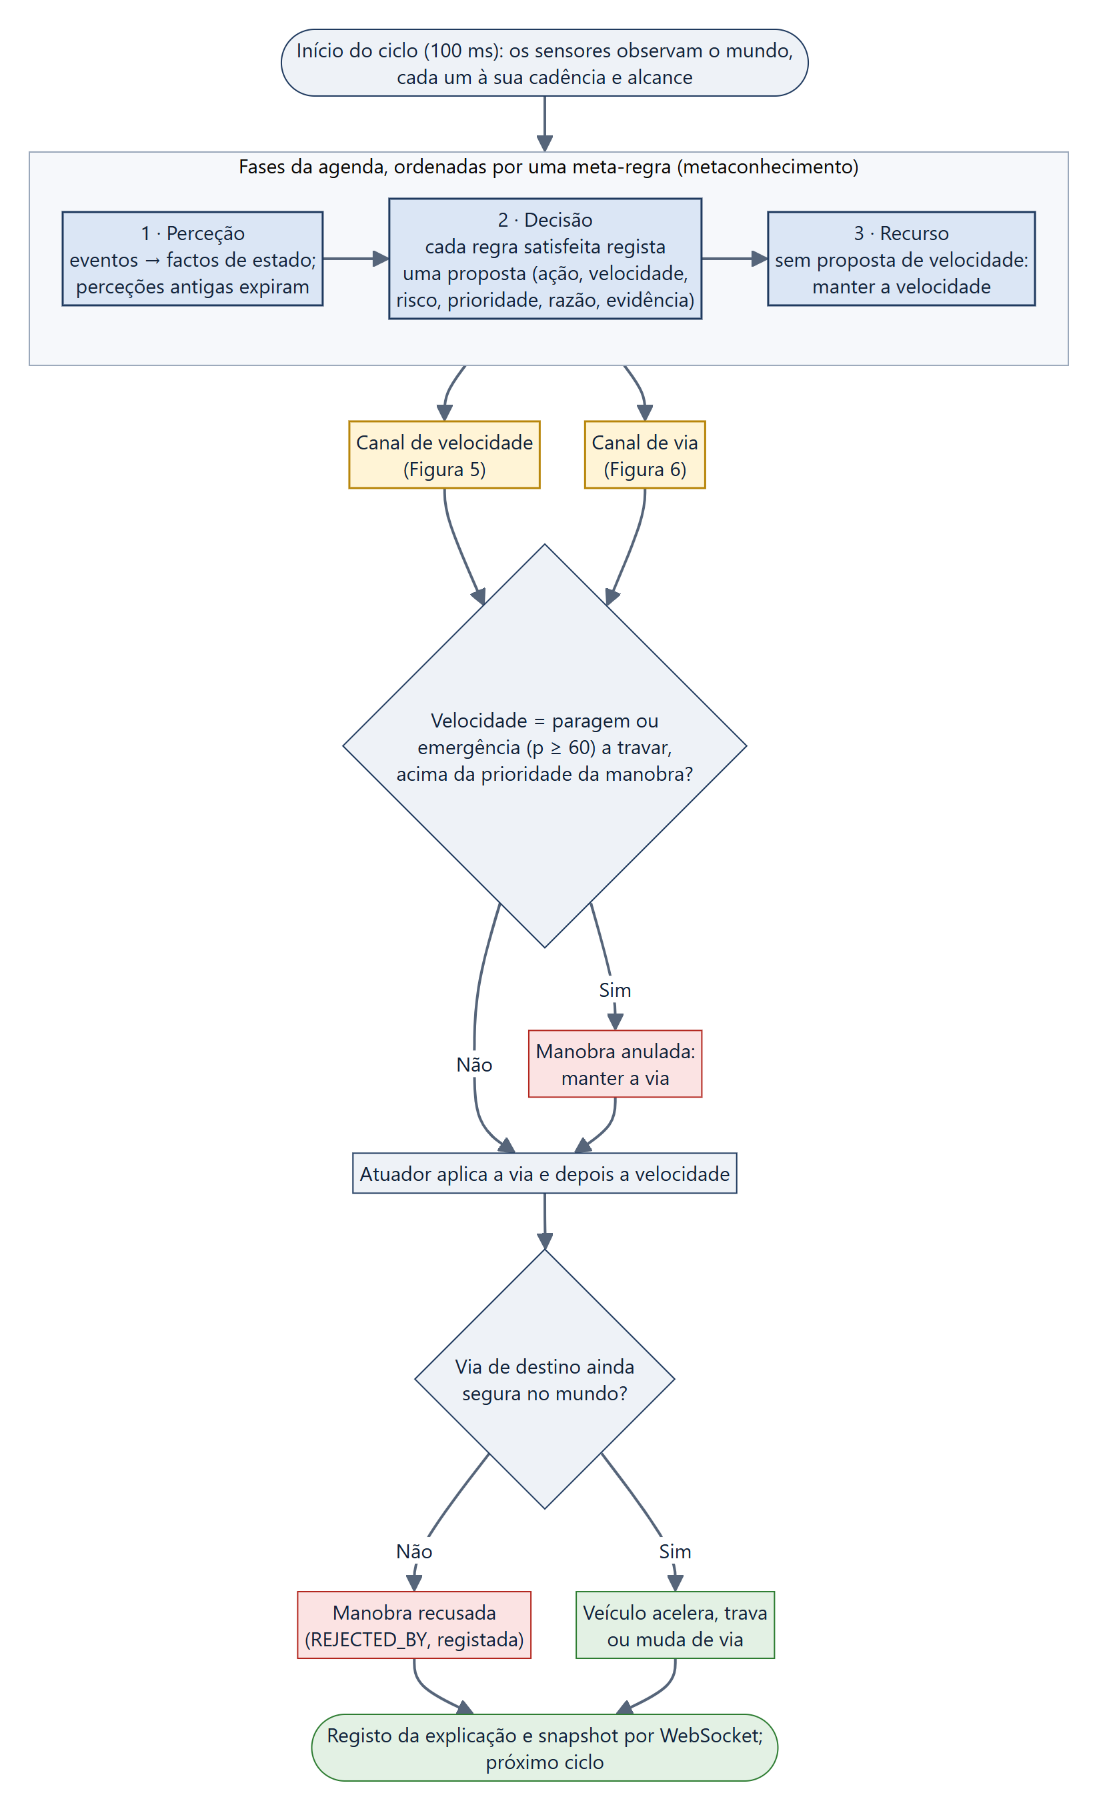
\includegraphics[width=\textwidth,height=0.92\textheight,keepaspectratio]{figuras/ciclo_decisao.png}
\caption{Fluxograma de inferência e decisão em cada ciclo de 100 ms}
\label{fig:ciclo-decisao}
\end{figure}

As Figuras 5 e 6 detalham, para cada canal, as perguntas pela ordem de importância. A travagem de emergência está no canal de velocidade e nunca passa pela pergunta ``a manobra é permitida?».

\begin{figure}[p]
\centering
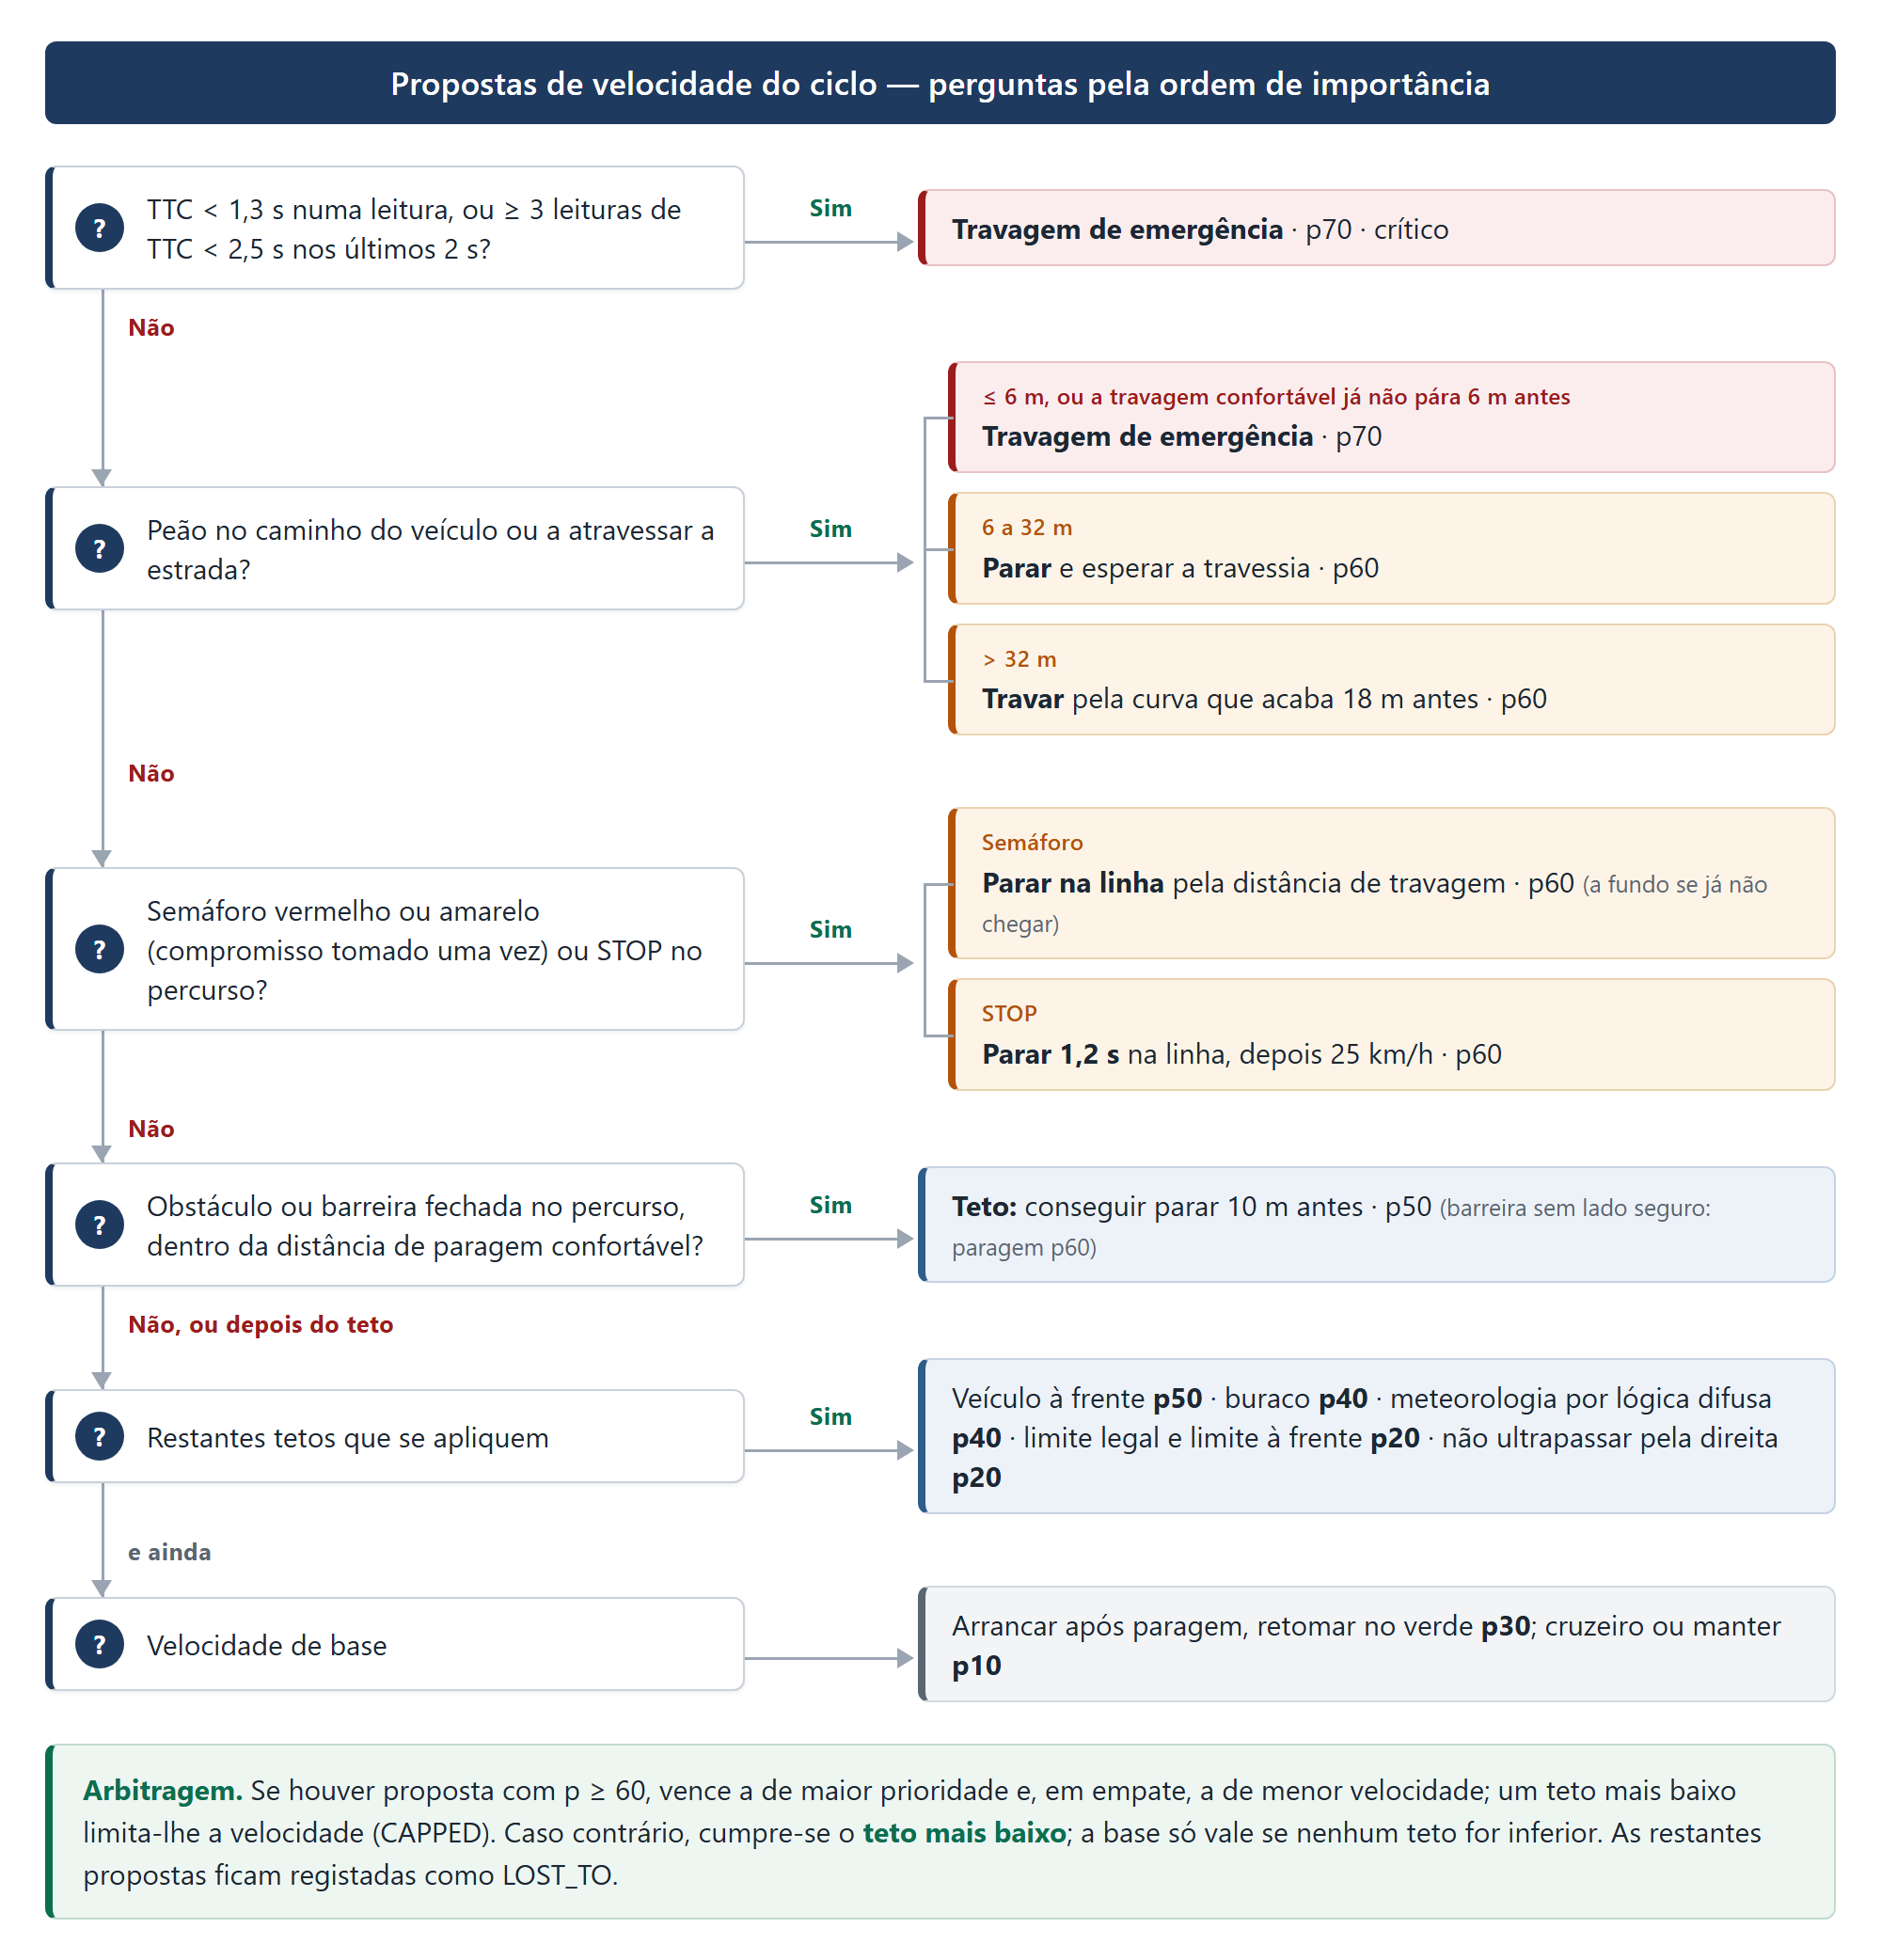
\includegraphics[width=\textwidth,height=0.92\textheight,keepaspectratio]{figuras/canal_velocidade.png}
\caption{Canal de velocidade: perguntas pela ordem de importância e arbitragem}
\label{fig:canal-velocidade}
\end{figure}

\begin{figure}[p]
\centering
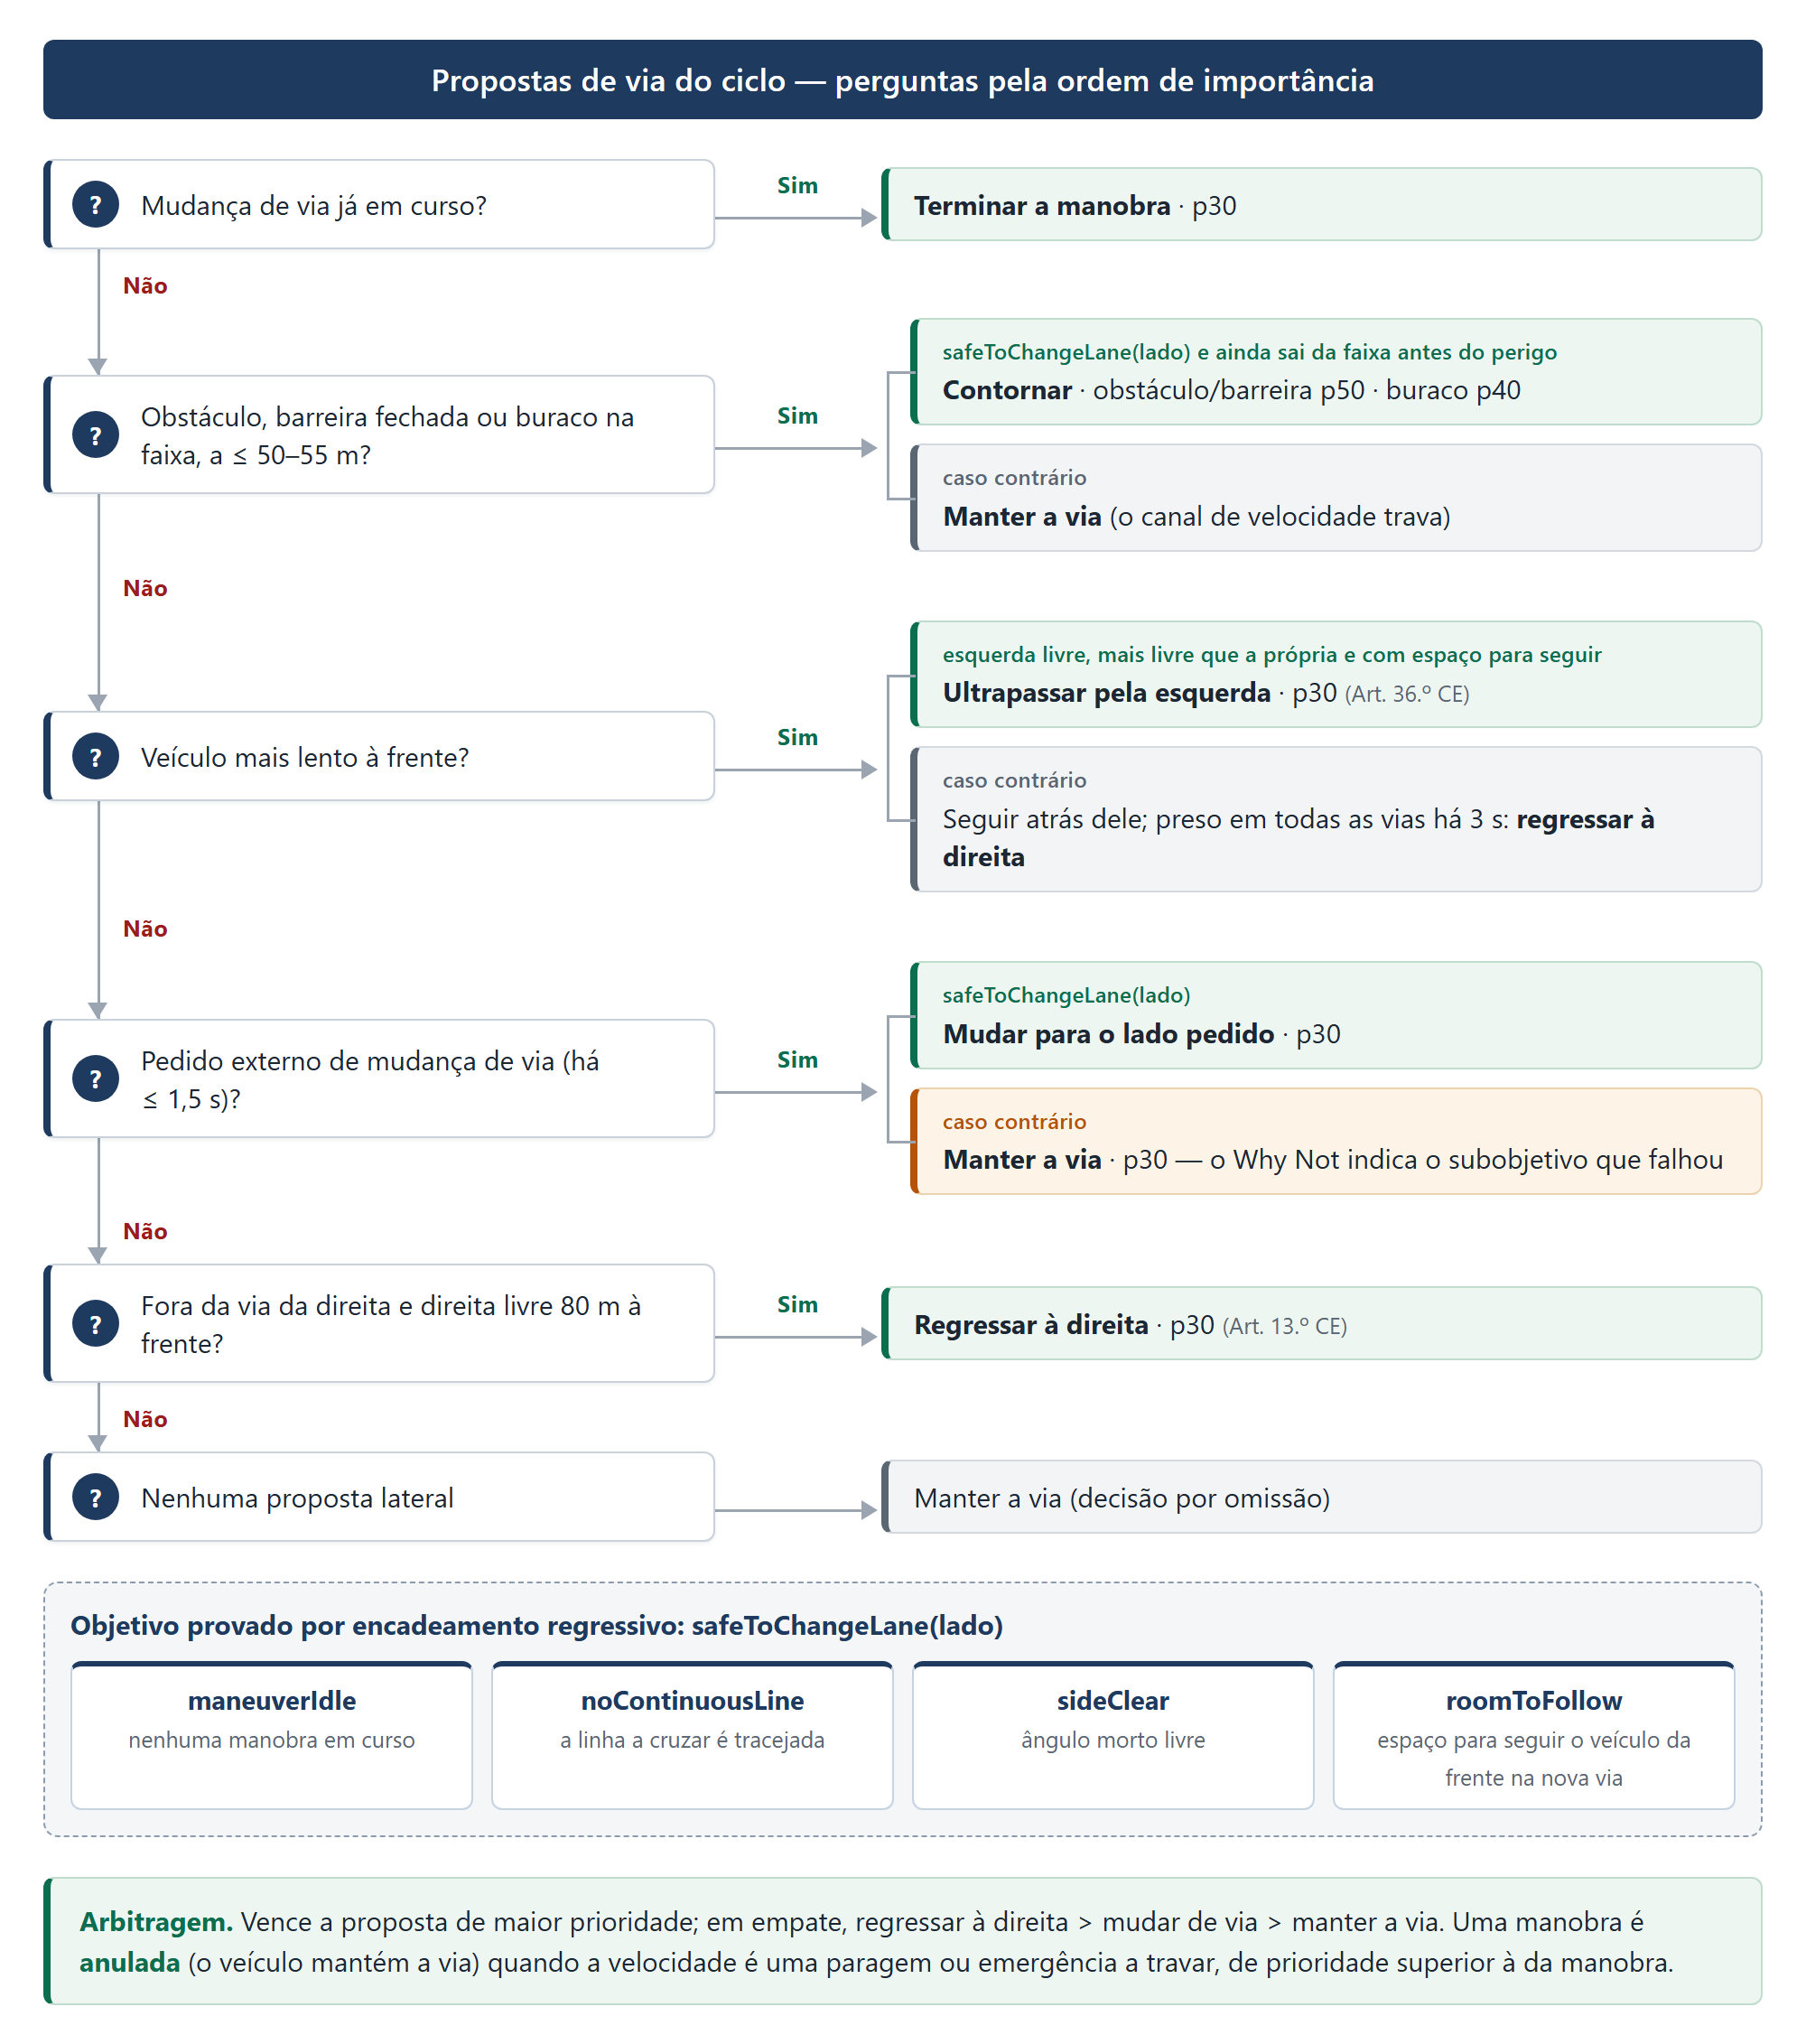
\includegraphics[width=\textwidth,height=0.92\textheight,keepaspectratio]{figuras/canal_via.png}
\caption{Canal de via e objetivo provado por encadeamento regressivo}
\label{fig:canal-via}
\end{figure}

\FloatBarrier
\section{Fluxograma completo}\label{sec:fluxograma-completo}

As Figuras 4 a 6 resumem o processo de decisão. A Figura 7 apresenta-o por inteiro: 49 perguntas e 43 ações, repetidas em cada ciclo de 100 ms. Para facilitar a leitura, o fluxograma foi dividido em sete zonas, cada uma com uma cor. As zonas A a E formam o canal de velocidade, as zonas F e G o canal de via, e a zona G termina com a atuação. Cada zona é ampliada numa figura própria (Figuras 8 a 14). No canto de cada ampliação, um pequeno mapa indica a zona em que o leitor se encontra, e as caixas tracejadas indicam de onde vem e para onde segue o fluxo. A versão vetorial do fluxograma completo, que pode ser ampliada sem perda de qualidade, é referida no Anexo B.

Este fluxograma deve ser lido como uma ordem de importância e não como uma sequência de execução. No Drools, todas as regras cujas condições se verificam disparam no mesmo ciclo e registam a sua proposta. A arbitragem descrita na Secção 5.1 escolhe depois a proposta vencedora. Como essa escolha segue as mesmas prioridades, o resultado é igual ao de percorrer o fluxograma de cima para baixo. Os hexágonos representam perguntas, os retângulos verdes representam ações e os vermelhos representam travagens fortes ou manobras canceladas.

\begin{sidewaysfigure}
\centering
\includegraphics[width=\textheight,height=0.92\textwidth,keepaspectratio]{figuras/fluxograma/fluxograma_completo.pdf}
\caption{Fluxograma completo do processo de decisão, dividido em zonas}
\label{fig:fluxo-completo}
\end{sidewaysfigure}

\begin{sidewaysfigure}
\begin{minipage}{\linewidth}
\noindent\textbf{Zona A -- Emergência e peões (\cref{fig:zonaA}).} É a primeira zona, porque trata
as situações em que está em causa uma colisão. Uma única leitura de TTC inferior a 1,3 s, ou três
leituras inferiores a 2,5 s nos últimos 2 s, origina uma travagem de emergência com luzes de
emergência (prioridade 70). Se houver um peão no caminho do veículo, a resposta depende da
distância. A 6 m ou menos, ou quando a travagem confortável já não permite parar 6 m antes, trava a
fundo. Entre 6 e 32 m, pára e espera que o peão termine a travessia. A mais de 32 m, abranda para
conseguir parar 18 m antes. Um obstáculo grave a 8 m ou menos, na via em que o veículo circula,
também origina uma emergência. A travagem de emergência termina diretamente na decisão de
velocidade e nunca passa por uma avaliação de manobra.
\end{minipage}

\vspace{4mm}
\centering
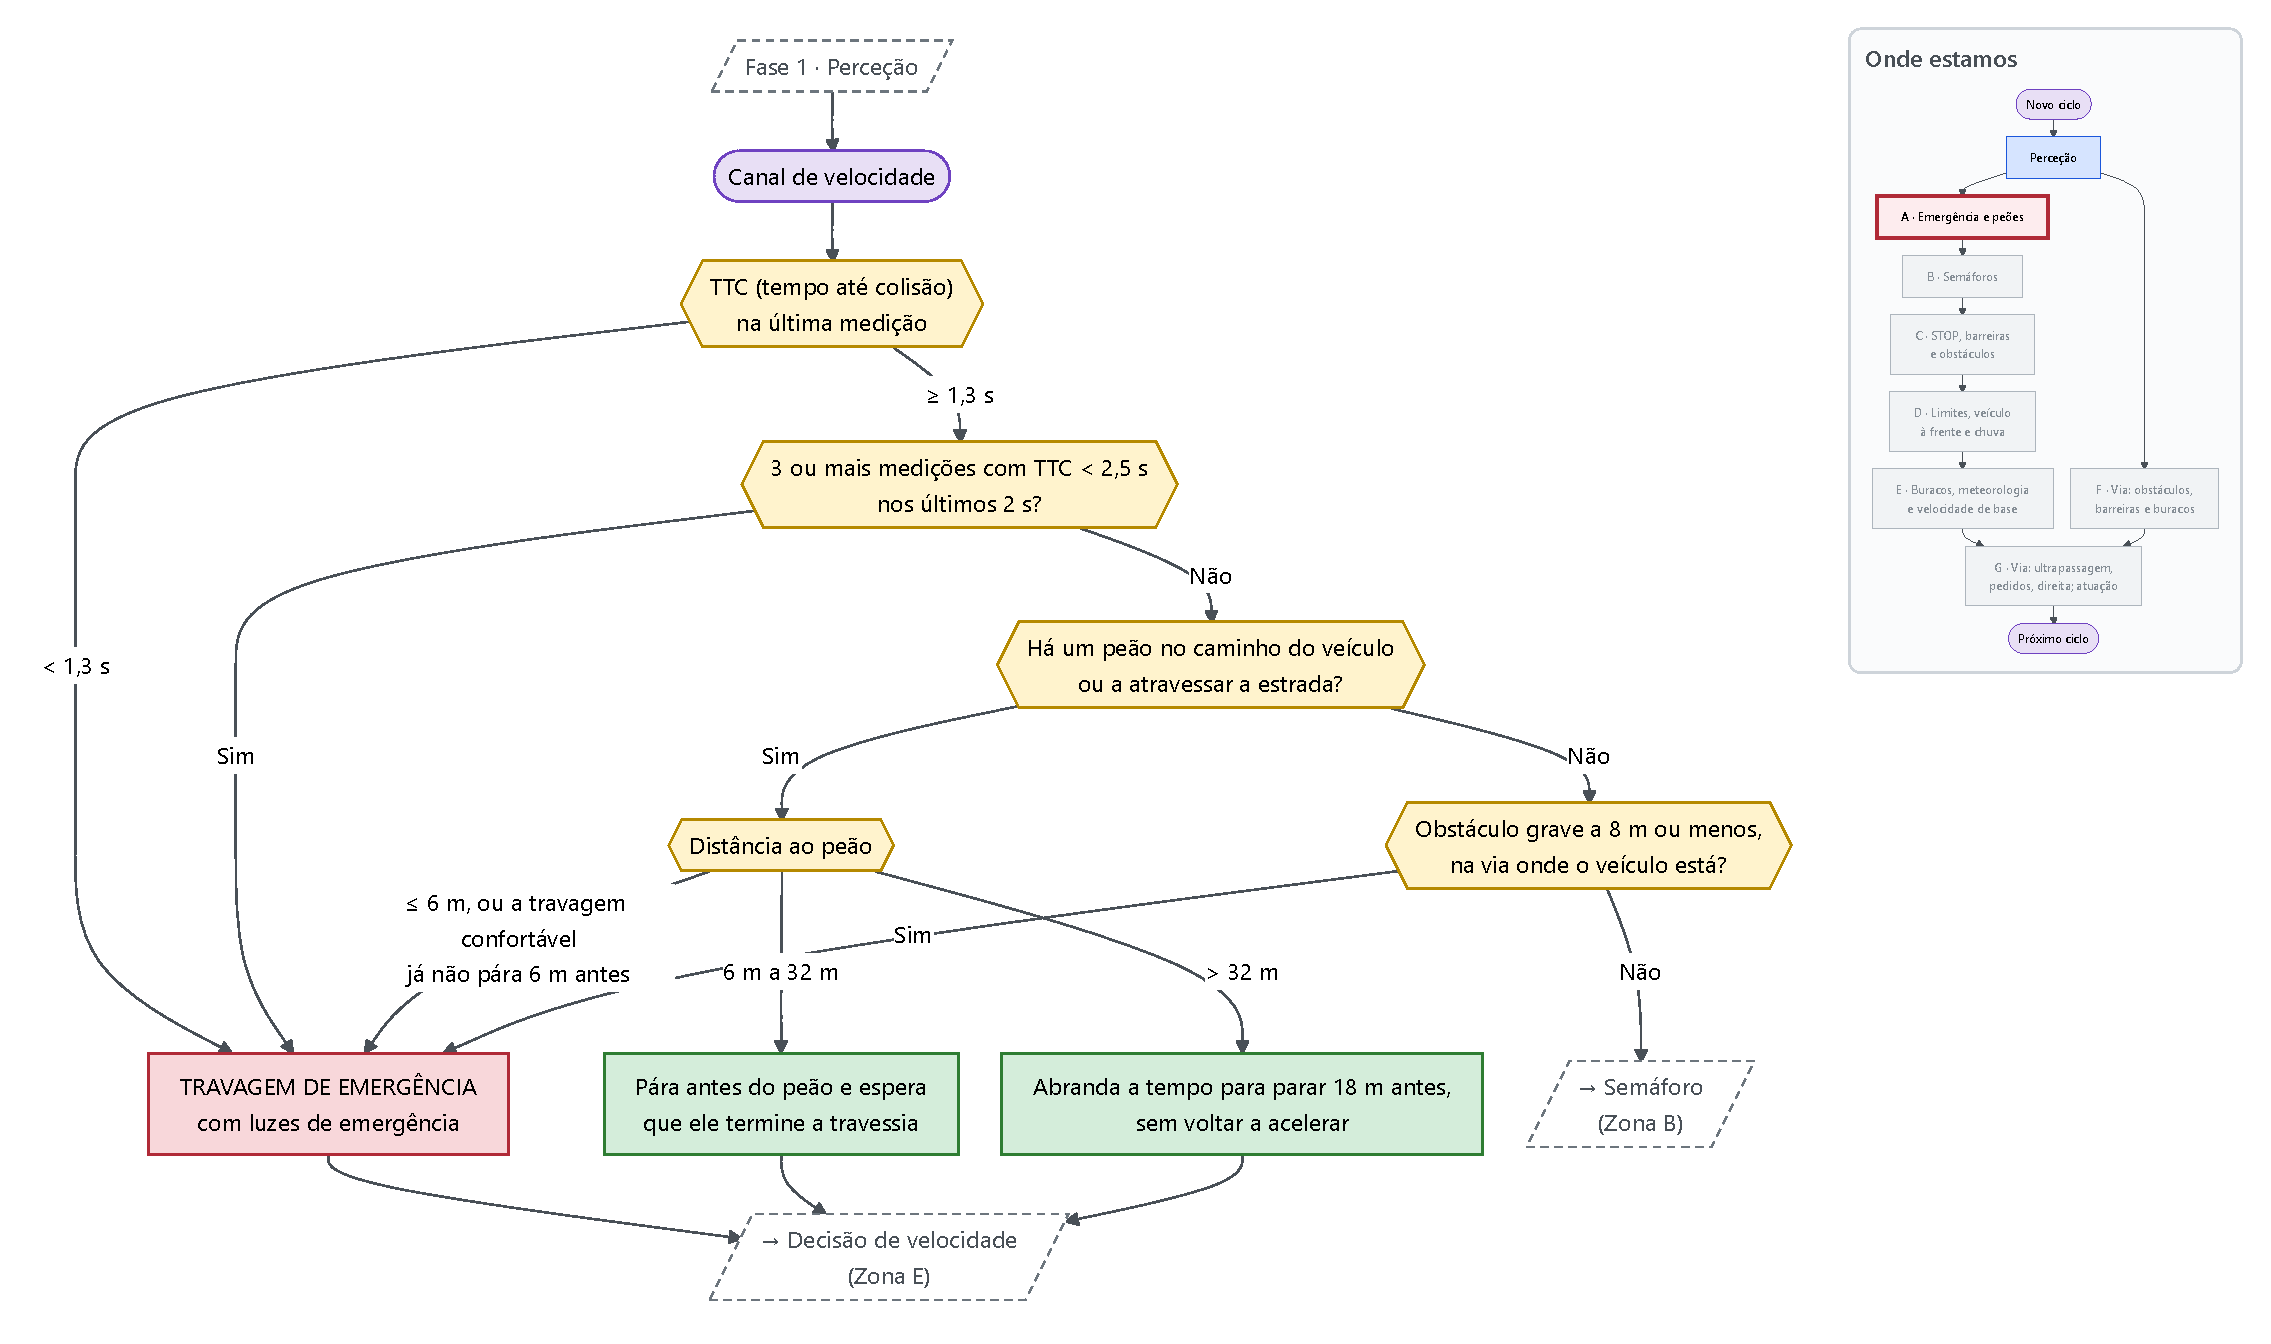
\includegraphics[width=\textheight,height=0.62\textwidth,keepaspectratio]{figuras/fluxograma/zona_A.pdf}
\caption{Zona A: emergência e peões}
\label{fig:zonaA}
\end{sidewaysfigure}

\begin{sidewaysfigure}
\begin{minipage}{\linewidth}
\noindent\textbf{Zona B -- Semáforos (\cref{fig:zonaB}).} Perante um semáforo vermelho, o veículo
compara a distância à linha com a distância de que precisa para parar: 0,5 s de reação, mais a
travagem, mais 18 m. Se estiver longe, continua. Se estiver na zona de transição, deixa de acelerar.
Se já estiver dentro da distância de travagem, trava com conforto (2,8 m/s²) e pára na linha, ou
trava a fundo quando a travagem confortável o levaria mais de 2 m para lá da linha. No amarelo, a
decisão de parar ou prosseguir é tomada uma única vez, para evitar que o veículo hesite e trave a
meio do cruzamento. No verde, o veículo segue ou volta a arrancar.
\end{minipage}

\vspace{4mm}
\centering
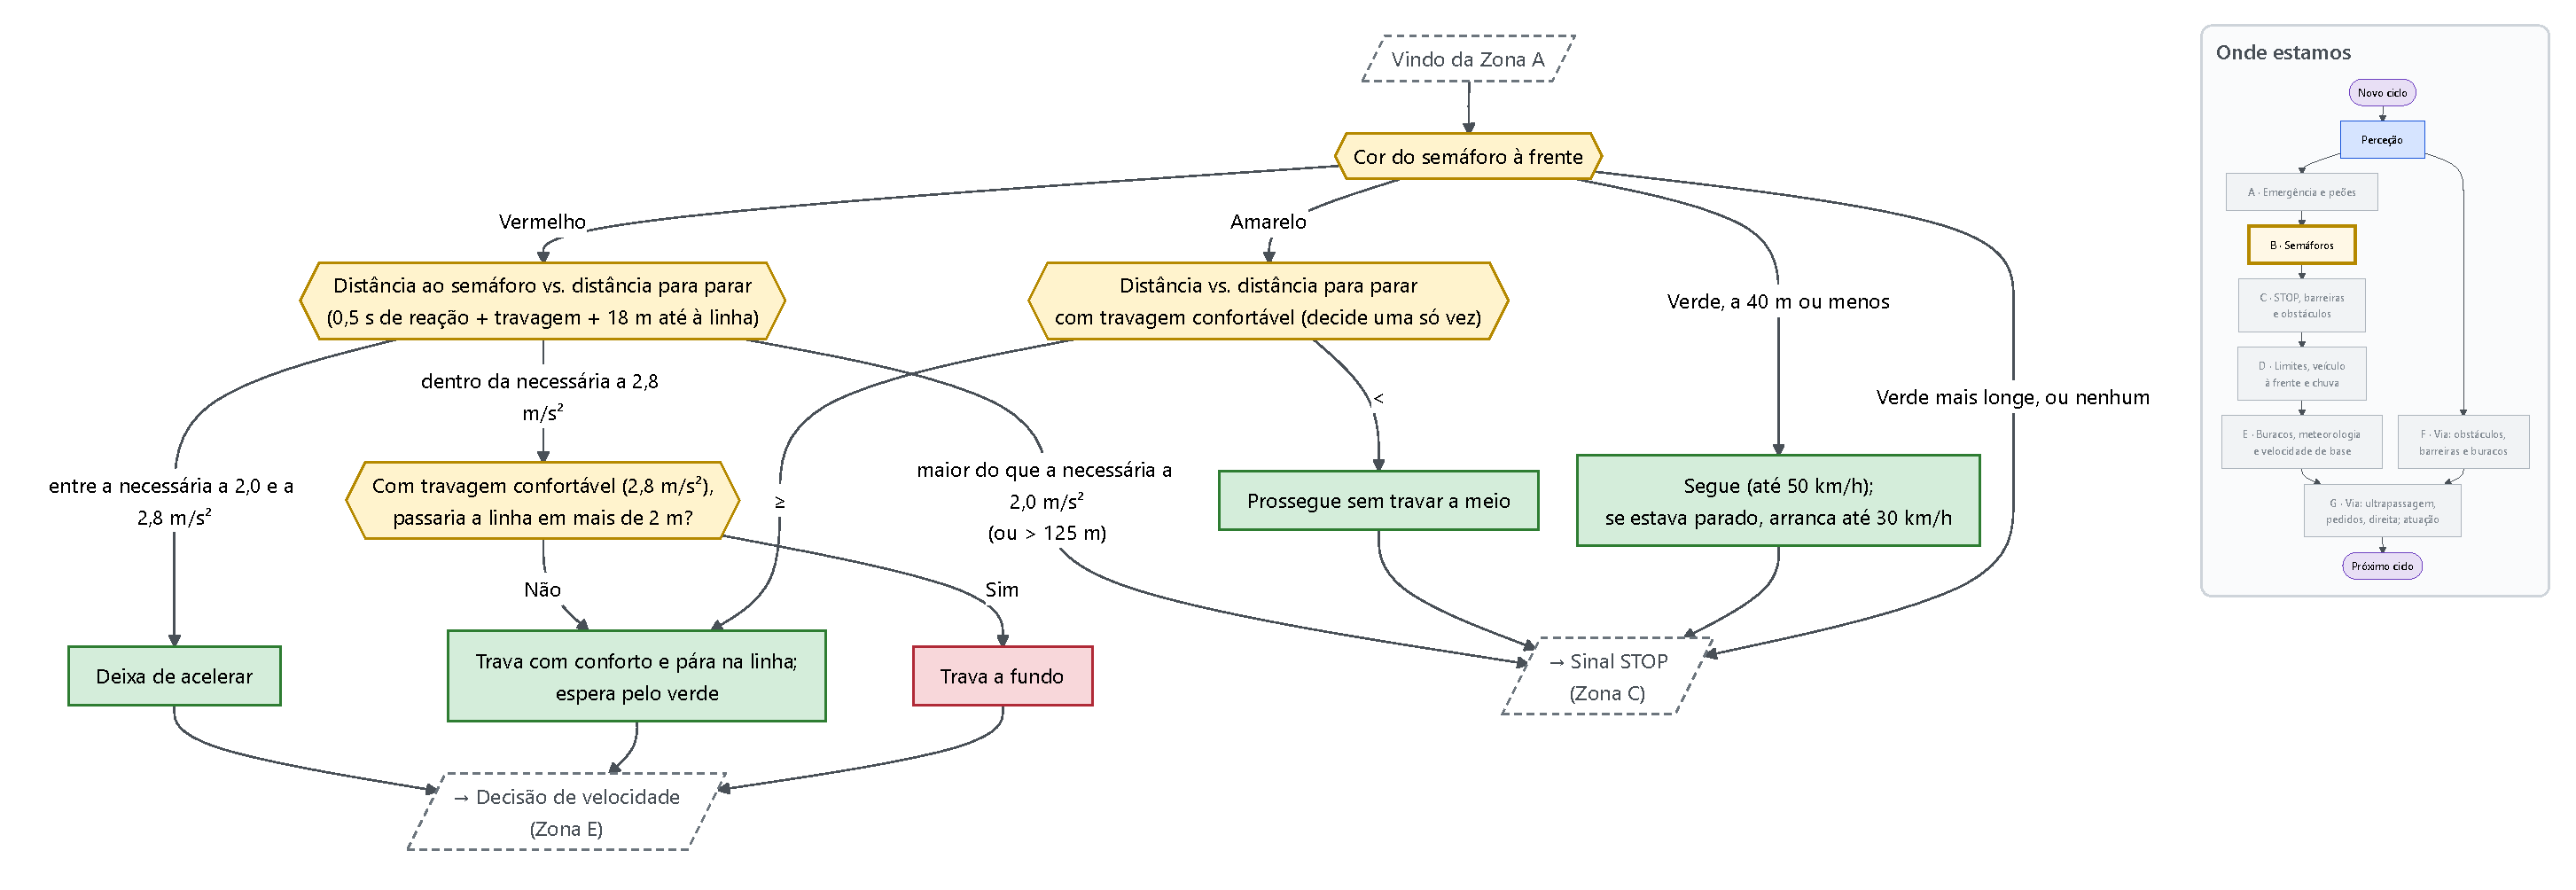
\includegraphics[width=\textheight,height=0.66\textwidth,keepaspectratio]{figuras/fluxograma/zona_B.pdf}
\caption{Zona B: semáforos}
\label{fig:zonaB}
\end{sidewaysfigure}

\begin{sidewaysfigure}
\begin{minipage}{\linewidth}
\noindent\textbf{Zona C -- STOP, barreiras e obstáculos (\cref{fig:zonaC}).} No sinal STOP, o
veículo pára na linha e só avança, a 25 km/h, depois de estar parado pelo menos 1,2 s, o que
garante a paragem completa exigida pelo Código da Estrada. Perante uma barreira fechada ou um
obstáculo dentro da distância de paragem confortável, o veículo trava para conseguir parar 10 m
antes. No caso da barreira, se for seguro mudar de via, essa travagem dura apenas até a mudança o
tirar do caminho. Se for preciso travar a mais de 3,1 m/s², a travagem passa a ser a fundo.
\end{minipage}

\vspace{4mm}
\centering
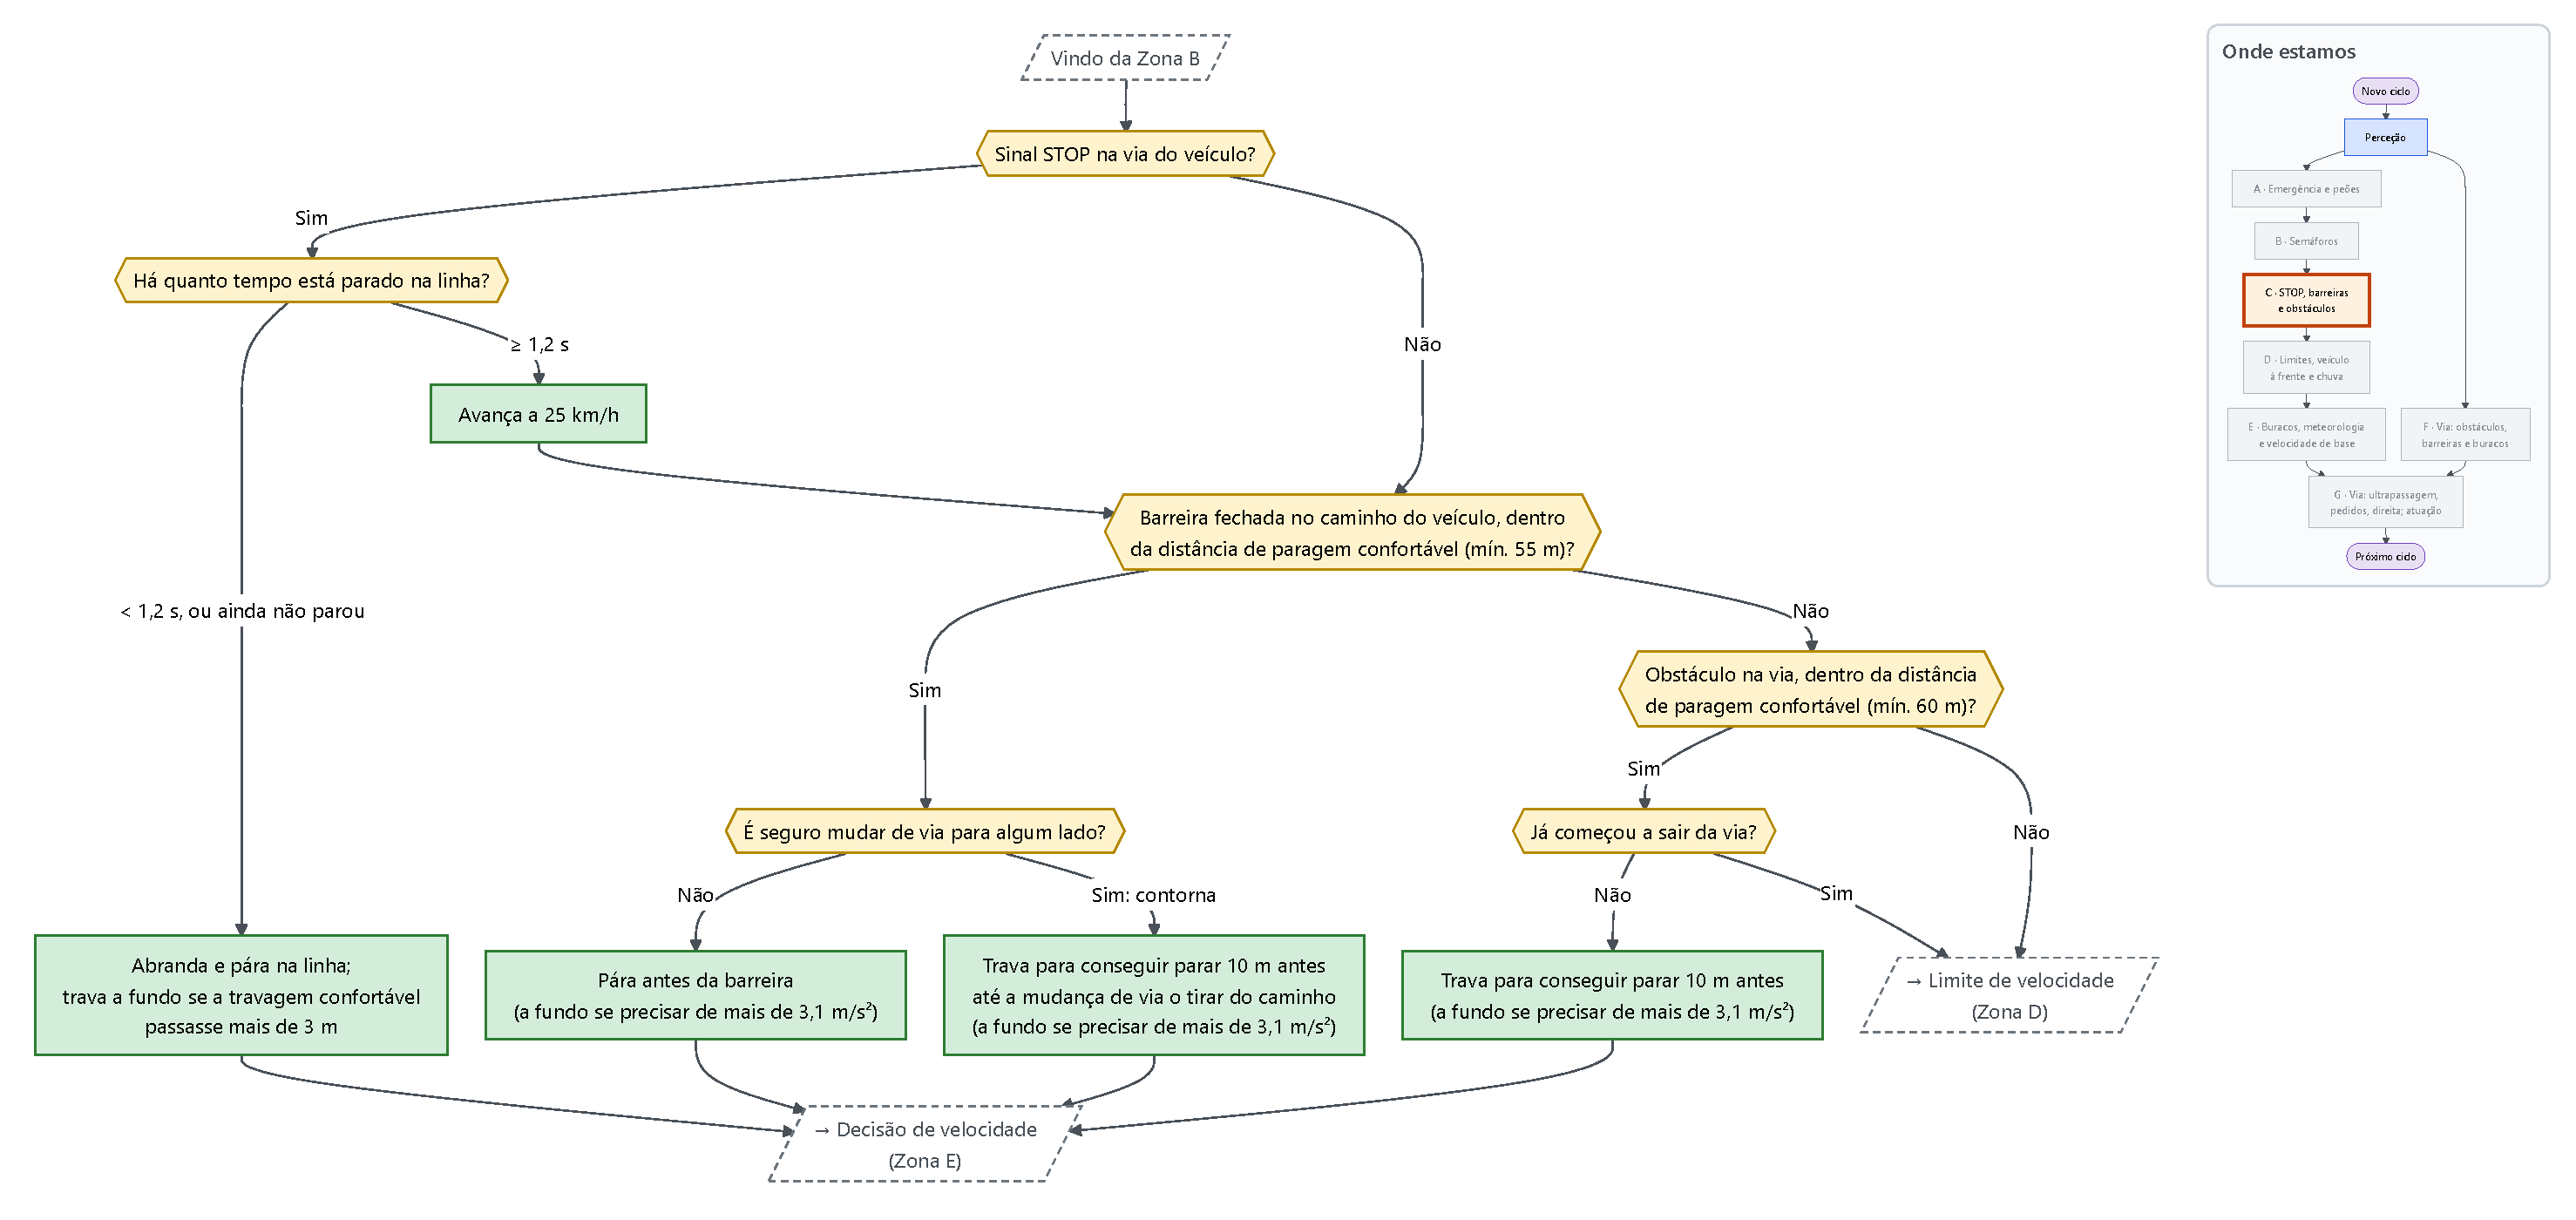
\includegraphics[width=\textheight,height=0.66\textwidth,keepaspectratio]{figuras/fluxograma/zona_C.pdf}
\caption{Zona C: STOP, barreiras e obstáculos}
\label{fig:zonaC}
\end{sidewaysfigure}

\clearpage
\noindent\textbf{Zona D -- Limites, veículo à frente e chuva (\cref{fig:zonaD}).} Esta zona produz
tetos de velocidade (prioridades 50 e 20), que se aplicam todos ao mesmo tempo. O veículo respeita
o limite em vigor e começa a abrandar a tempo de chegar ao sinal seguinte já com o novo limite,
travando a 2,0 m/s². Com um veículo à frente, pára cerca de 12 m atrás se este estiver parado. Se
estiver em movimento, abranda até 3 km/h abaixo dele, acompanha a sua velocidade ou abranda apenas
o necessário, conforme a distância. Com pouca aderência, essa distância duplica. O veículo não
ultrapassa pela direita um veículo mais lento na via da esquerda. Com chuva, duas leituras de TTC
inferiores a 3 s em 2 s levam o veículo a travar até 15 km/h.

\begin{figure}[H]
\centering
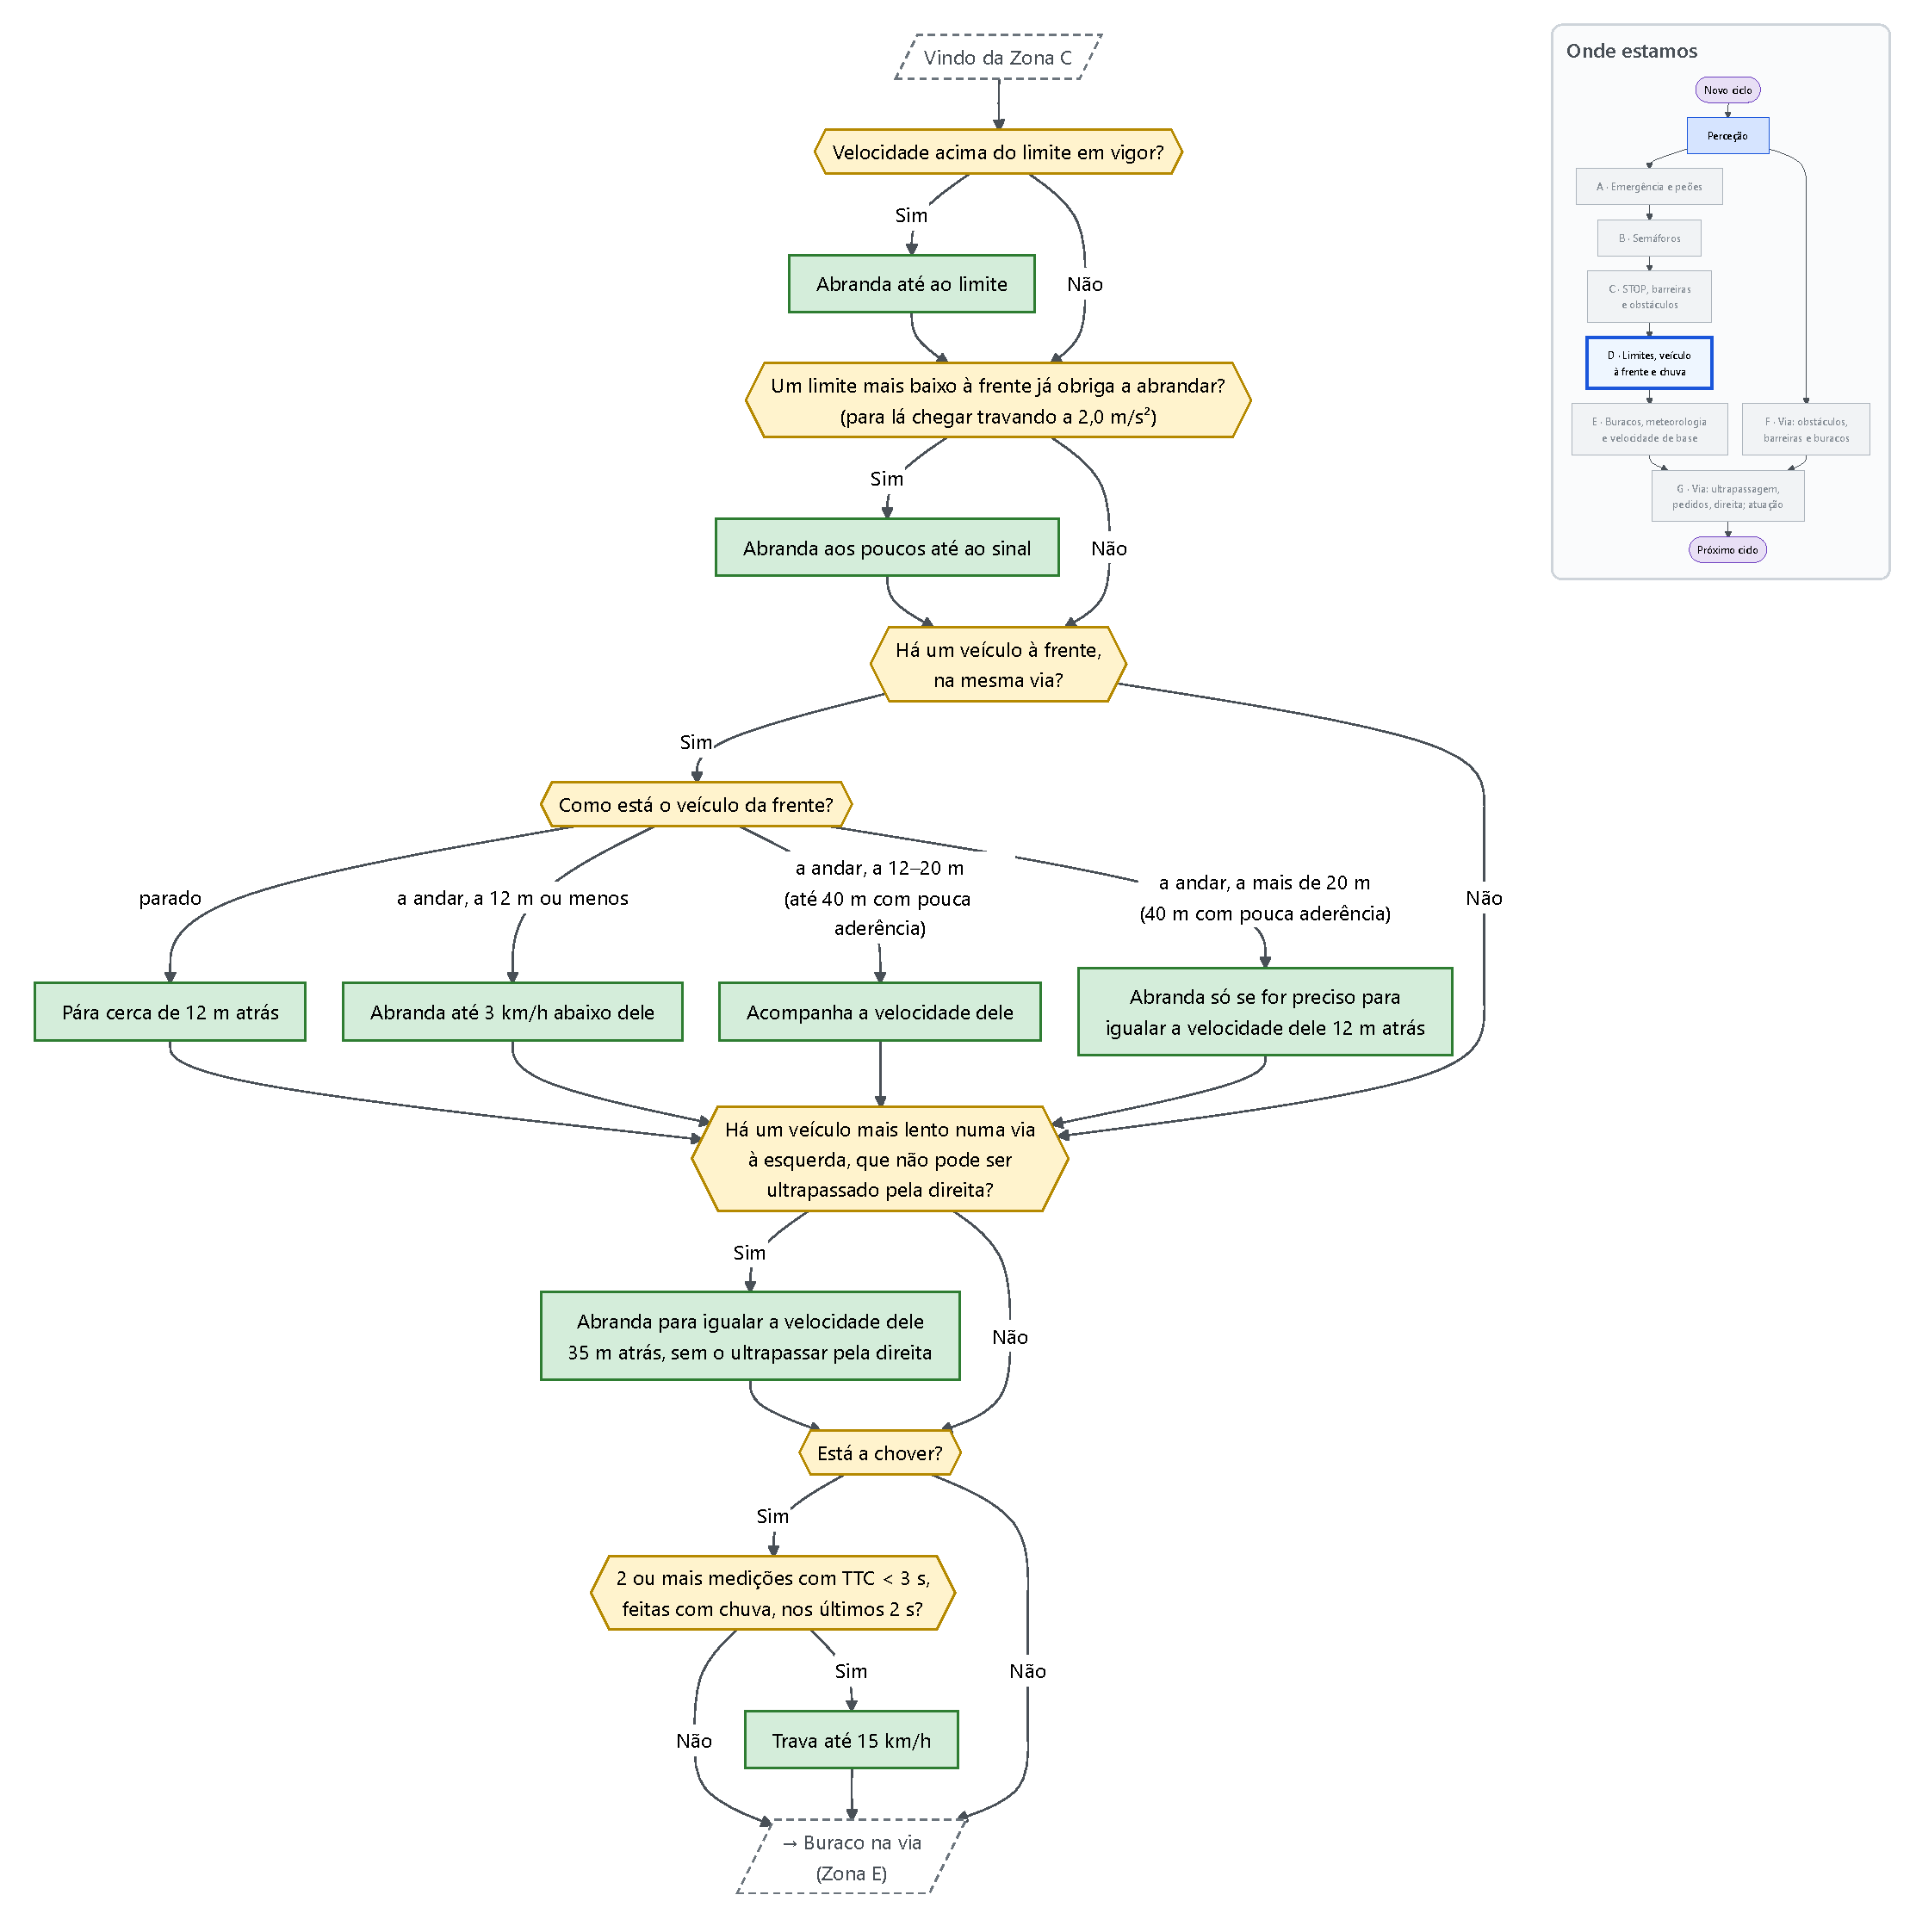
\includegraphics[width=\textwidth,height=0.70\textheight,keepaspectratio]{figuras/fluxograma/zona_D.pdf}
\caption{Zona D: limites, veículo à frente e chuva}
\label{fig:zonaD}
\end{figure}

\clearpage
\noindent\textbf{Zona E -- Buracos, meteorologia e velocidade de base (\cref{fig:zonaE}).} Se não
conseguir desviar-se de um buraco, o veículo passa por ele a 30 km/h, e a 20 km/h nos últimos 15 m.
Junto a uma barreira aberta, não passa de 35 km/h. Com chuva, visibilidade reduzida ou pouca
aderência, a lógica difusa calcula uma velocidade máxima recomendada, entre cerca de 25 e pouco
mais de 70 km/h. Só depois de considerados todos os tetos é definida a velocidade de base: arrancar
após uma paragem, acelerar a pedido, manter o limite do sinal ou retomar a velocidade de cruzeiro.
Se nenhuma regra se aplicar, a fase de recurso mantém a velocidade. Por fim, vale a velocidade mais
baixa entre a de base e todos os tetos encontrados, pelo que o veículo nunca ultrapassa o limite
legal.

\begin{figure}[H]
\centering
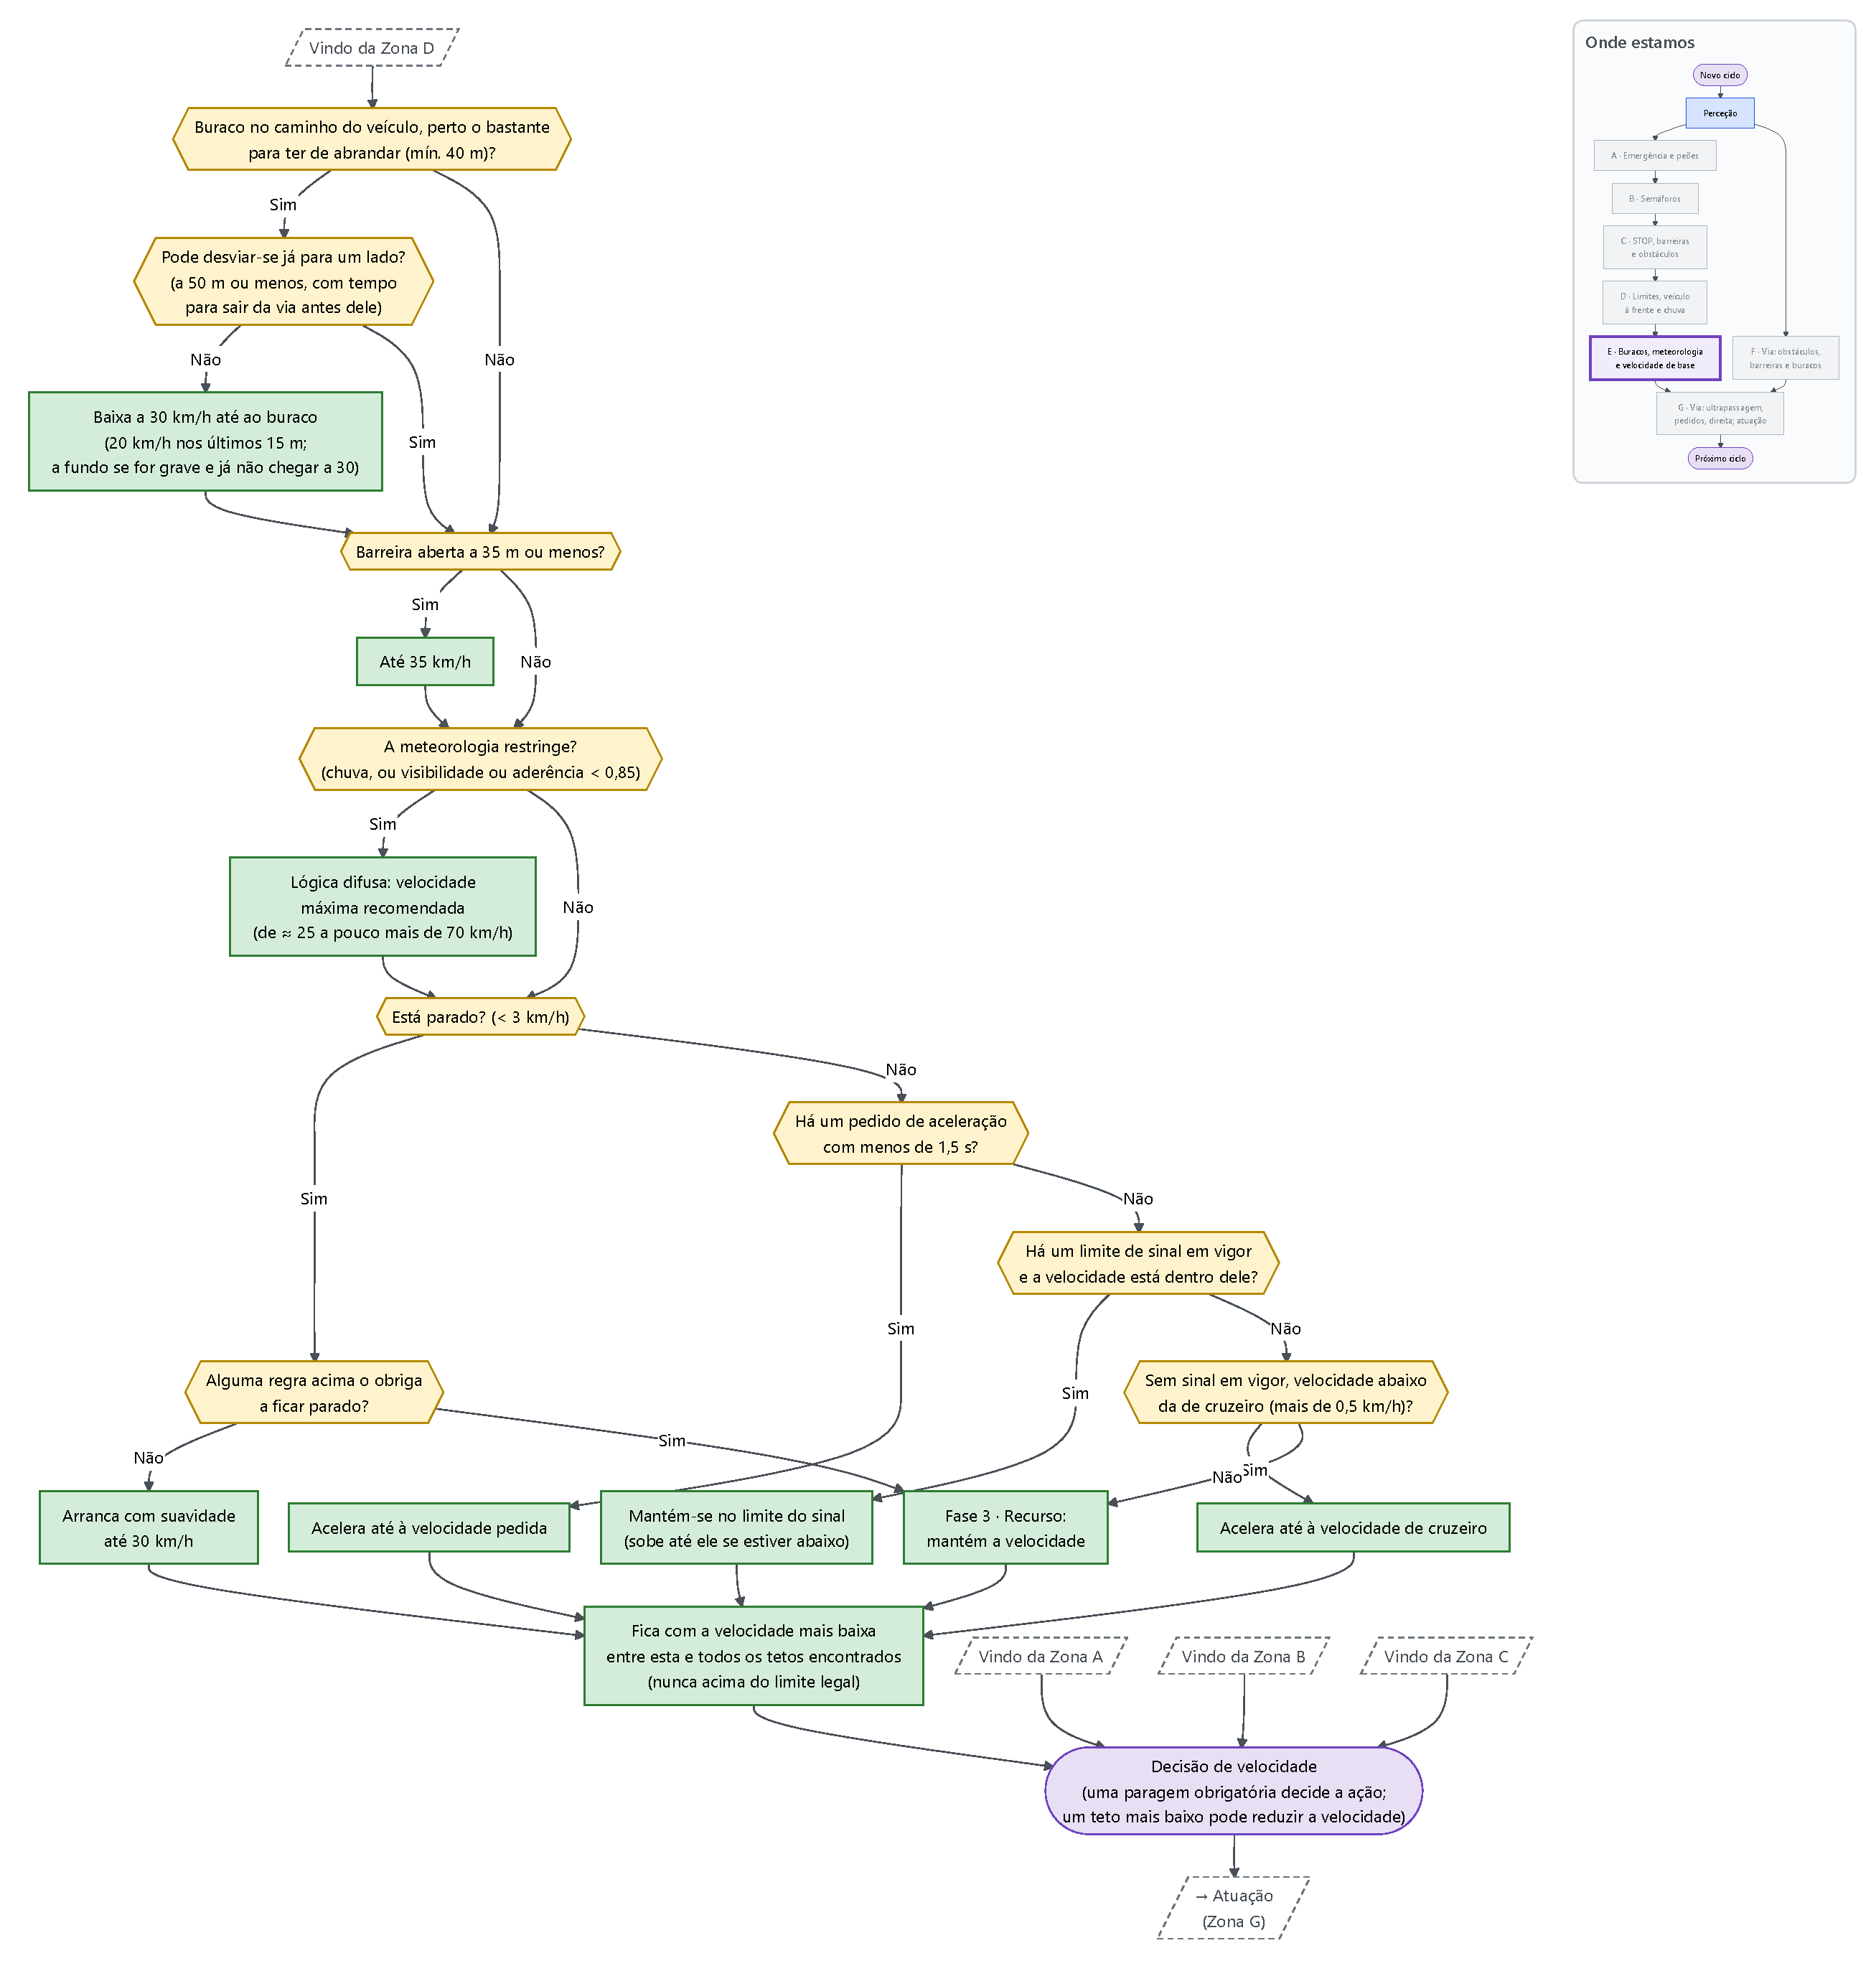
\includegraphics[width=\textwidth,height=0.70\textheight,keepaspectratio]{figuras/fluxograma/zona_E.pdf}
\caption{Zona E: buracos, meteorologia e velocidade de base}
\label{fig:zonaE}
\end{figure}

\clearpage
\begin{sidewaysfigure}
\begin{minipage}{\linewidth}
\noindent\textbf{Zona F -- Via: obstáculos, barreiras e buracos (\cref{fig:zonaF}).} O canal de via
começa por confirmar se uma emergência ou paragem obrigatória está a travar o veículo. Se estiver,
o veículo mantém a via, o que garante que nenhuma manobra compete com uma travagem crítica. Uma
mudança de via já iniciada é sempre concluída. Perante um obstáculo, uma barreira fechada ou um
buraco na via, o veículo contorna-o se for seguro mudar de via e se ainda conseguir sair da via
antes de lá chegar. Caso contrário, mantém a via e o canal de velocidade trata da paragem ou da
passagem lenta.
\end{minipage}

\vspace{4mm}
\centering
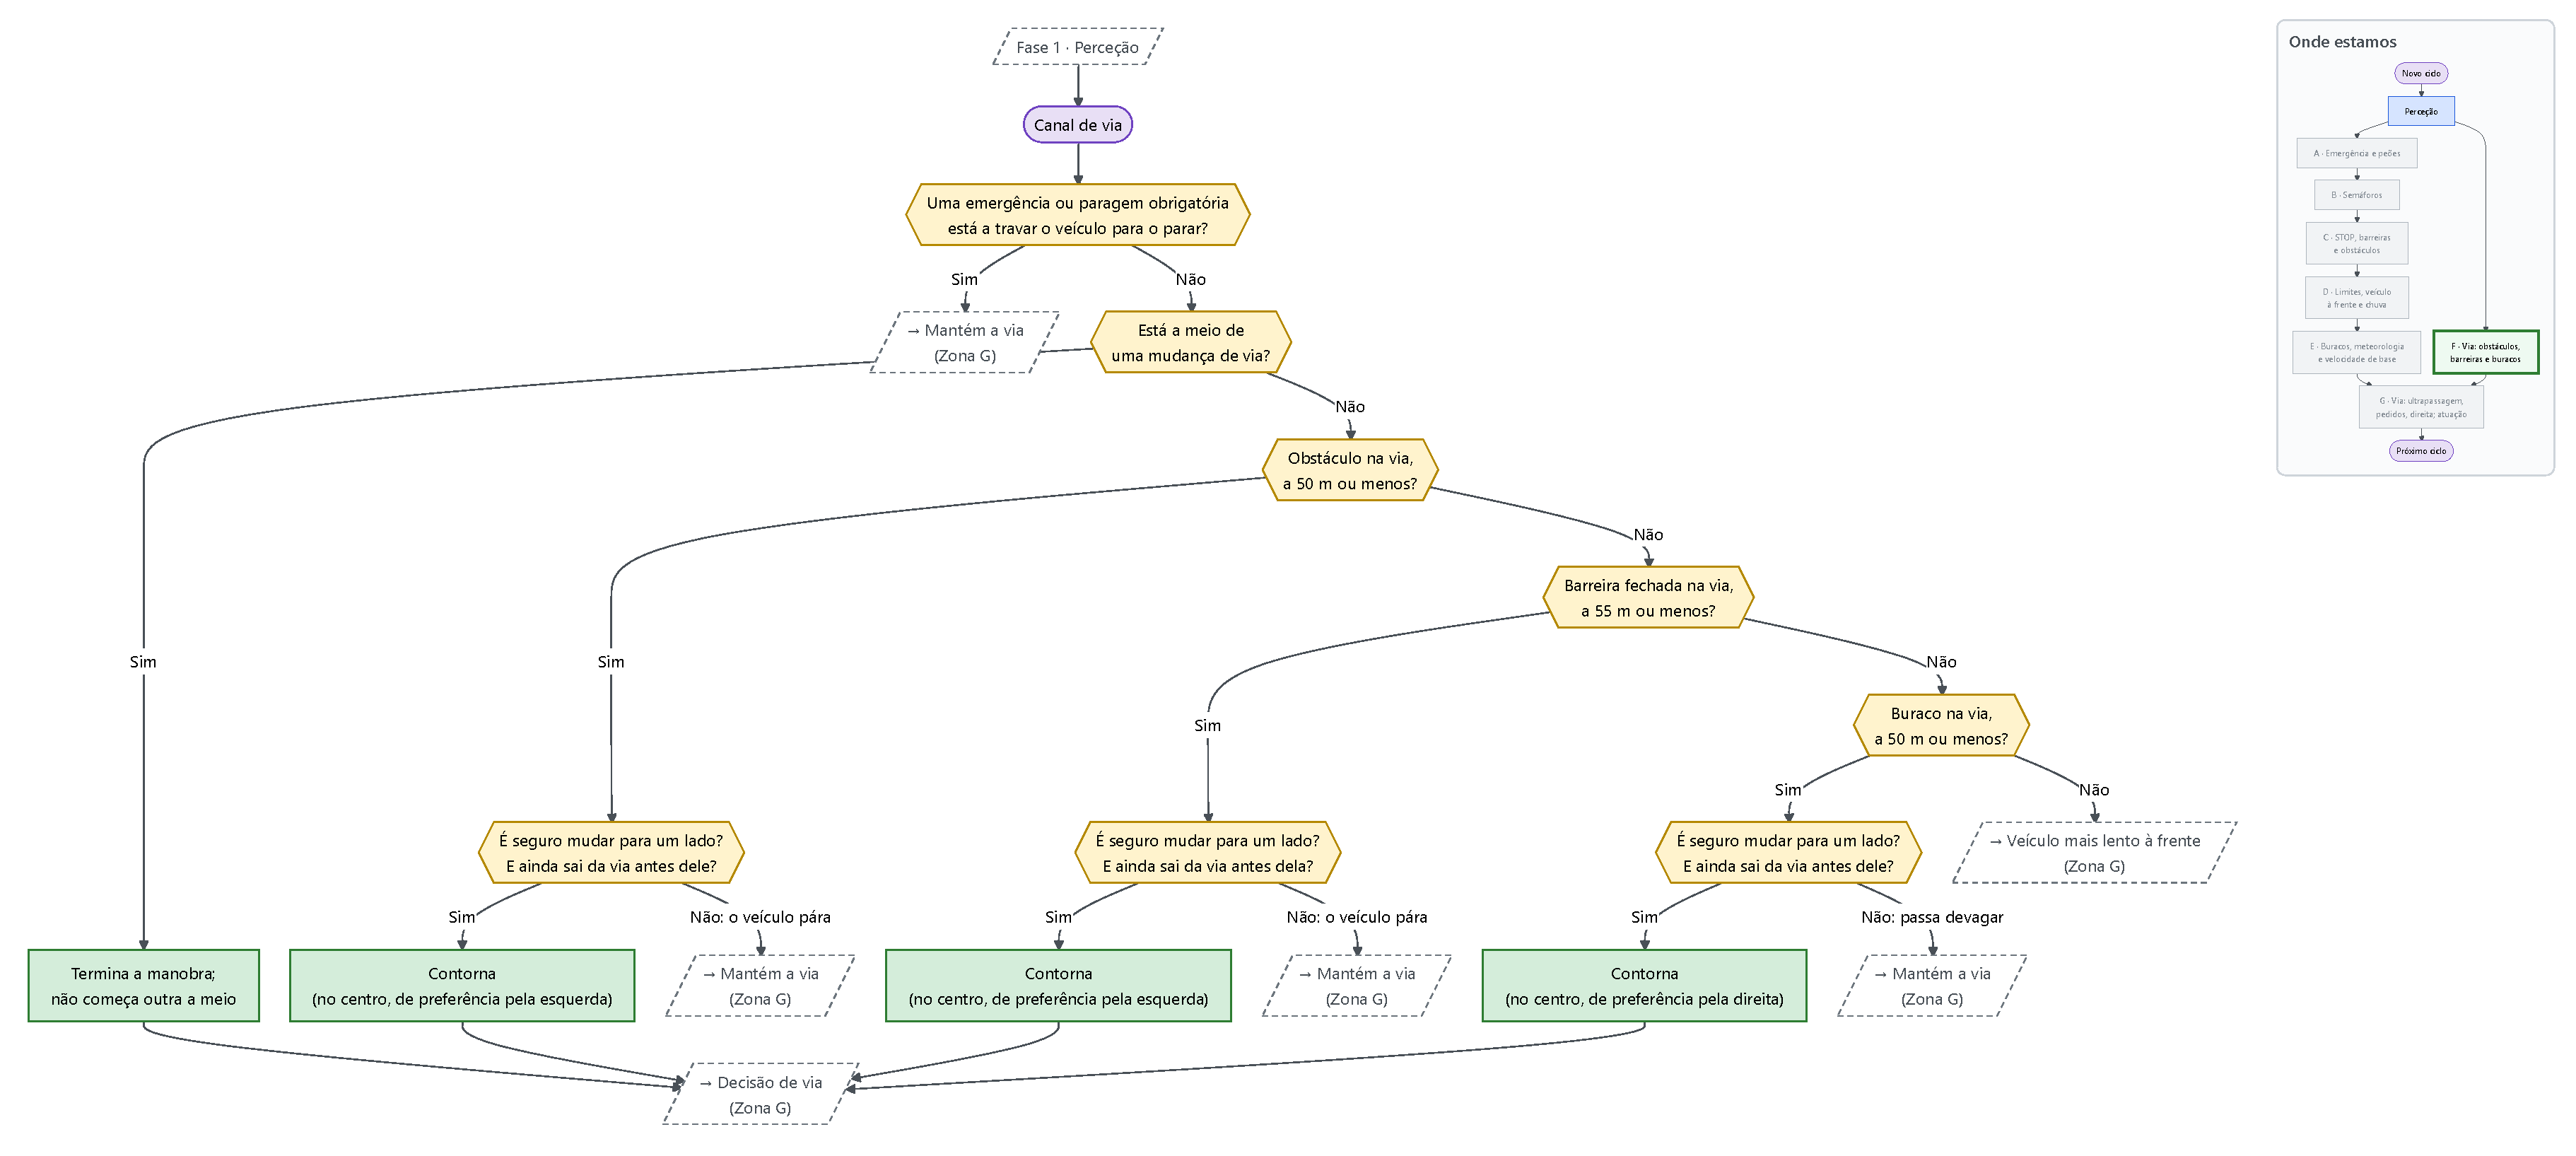
\includegraphics[width=\textheight,height=0.64\textwidth,keepaspectratio]{figuras/fluxograma/zona_F.pdf}
\caption{Zona F: canal de via perante obstáculos, barreiras e buracos}
\label{fig:zonaF}
\end{sidewaysfigure}

\begin{sidewaysfigure}
\begin{minipage}{\linewidth}
\noindent\textbf{Zona G -- Ultrapassagem, pedidos, regresso à direita e atuação
(\cref{fig:zonaG}).} Atrás de um veículo mais lento, o veículo ultrapassa apenas pela esquerda. Se
estiver preso atrás de trânsito lento em todas as vias há pelo menos 3 s, desiste e regressa à
direita. Um pedido externo de mudança de via só é aceite se a mudança for segura; se não for, é
recusado e a explicação indica qual das condições falhou. Sem outro motivo para ficar, o veículo
regressa à via da direita, uma via de cada vez, como determina o Código da Estrada. As decisões de
velocidade e de via juntam-se na atuação. Antes de iniciar uma mudança de via, o atuador volta a
confirmar no mundo que a via de destino está livre e que não há linha contínua. Se alguma destas
condições falhar, cancela a manobra e abranda 10 km/h. Por fim, ajusta a velocidade com suavidade e
começa o ciclo seguinte.
\end{minipage}

\vspace{4mm}
\centering
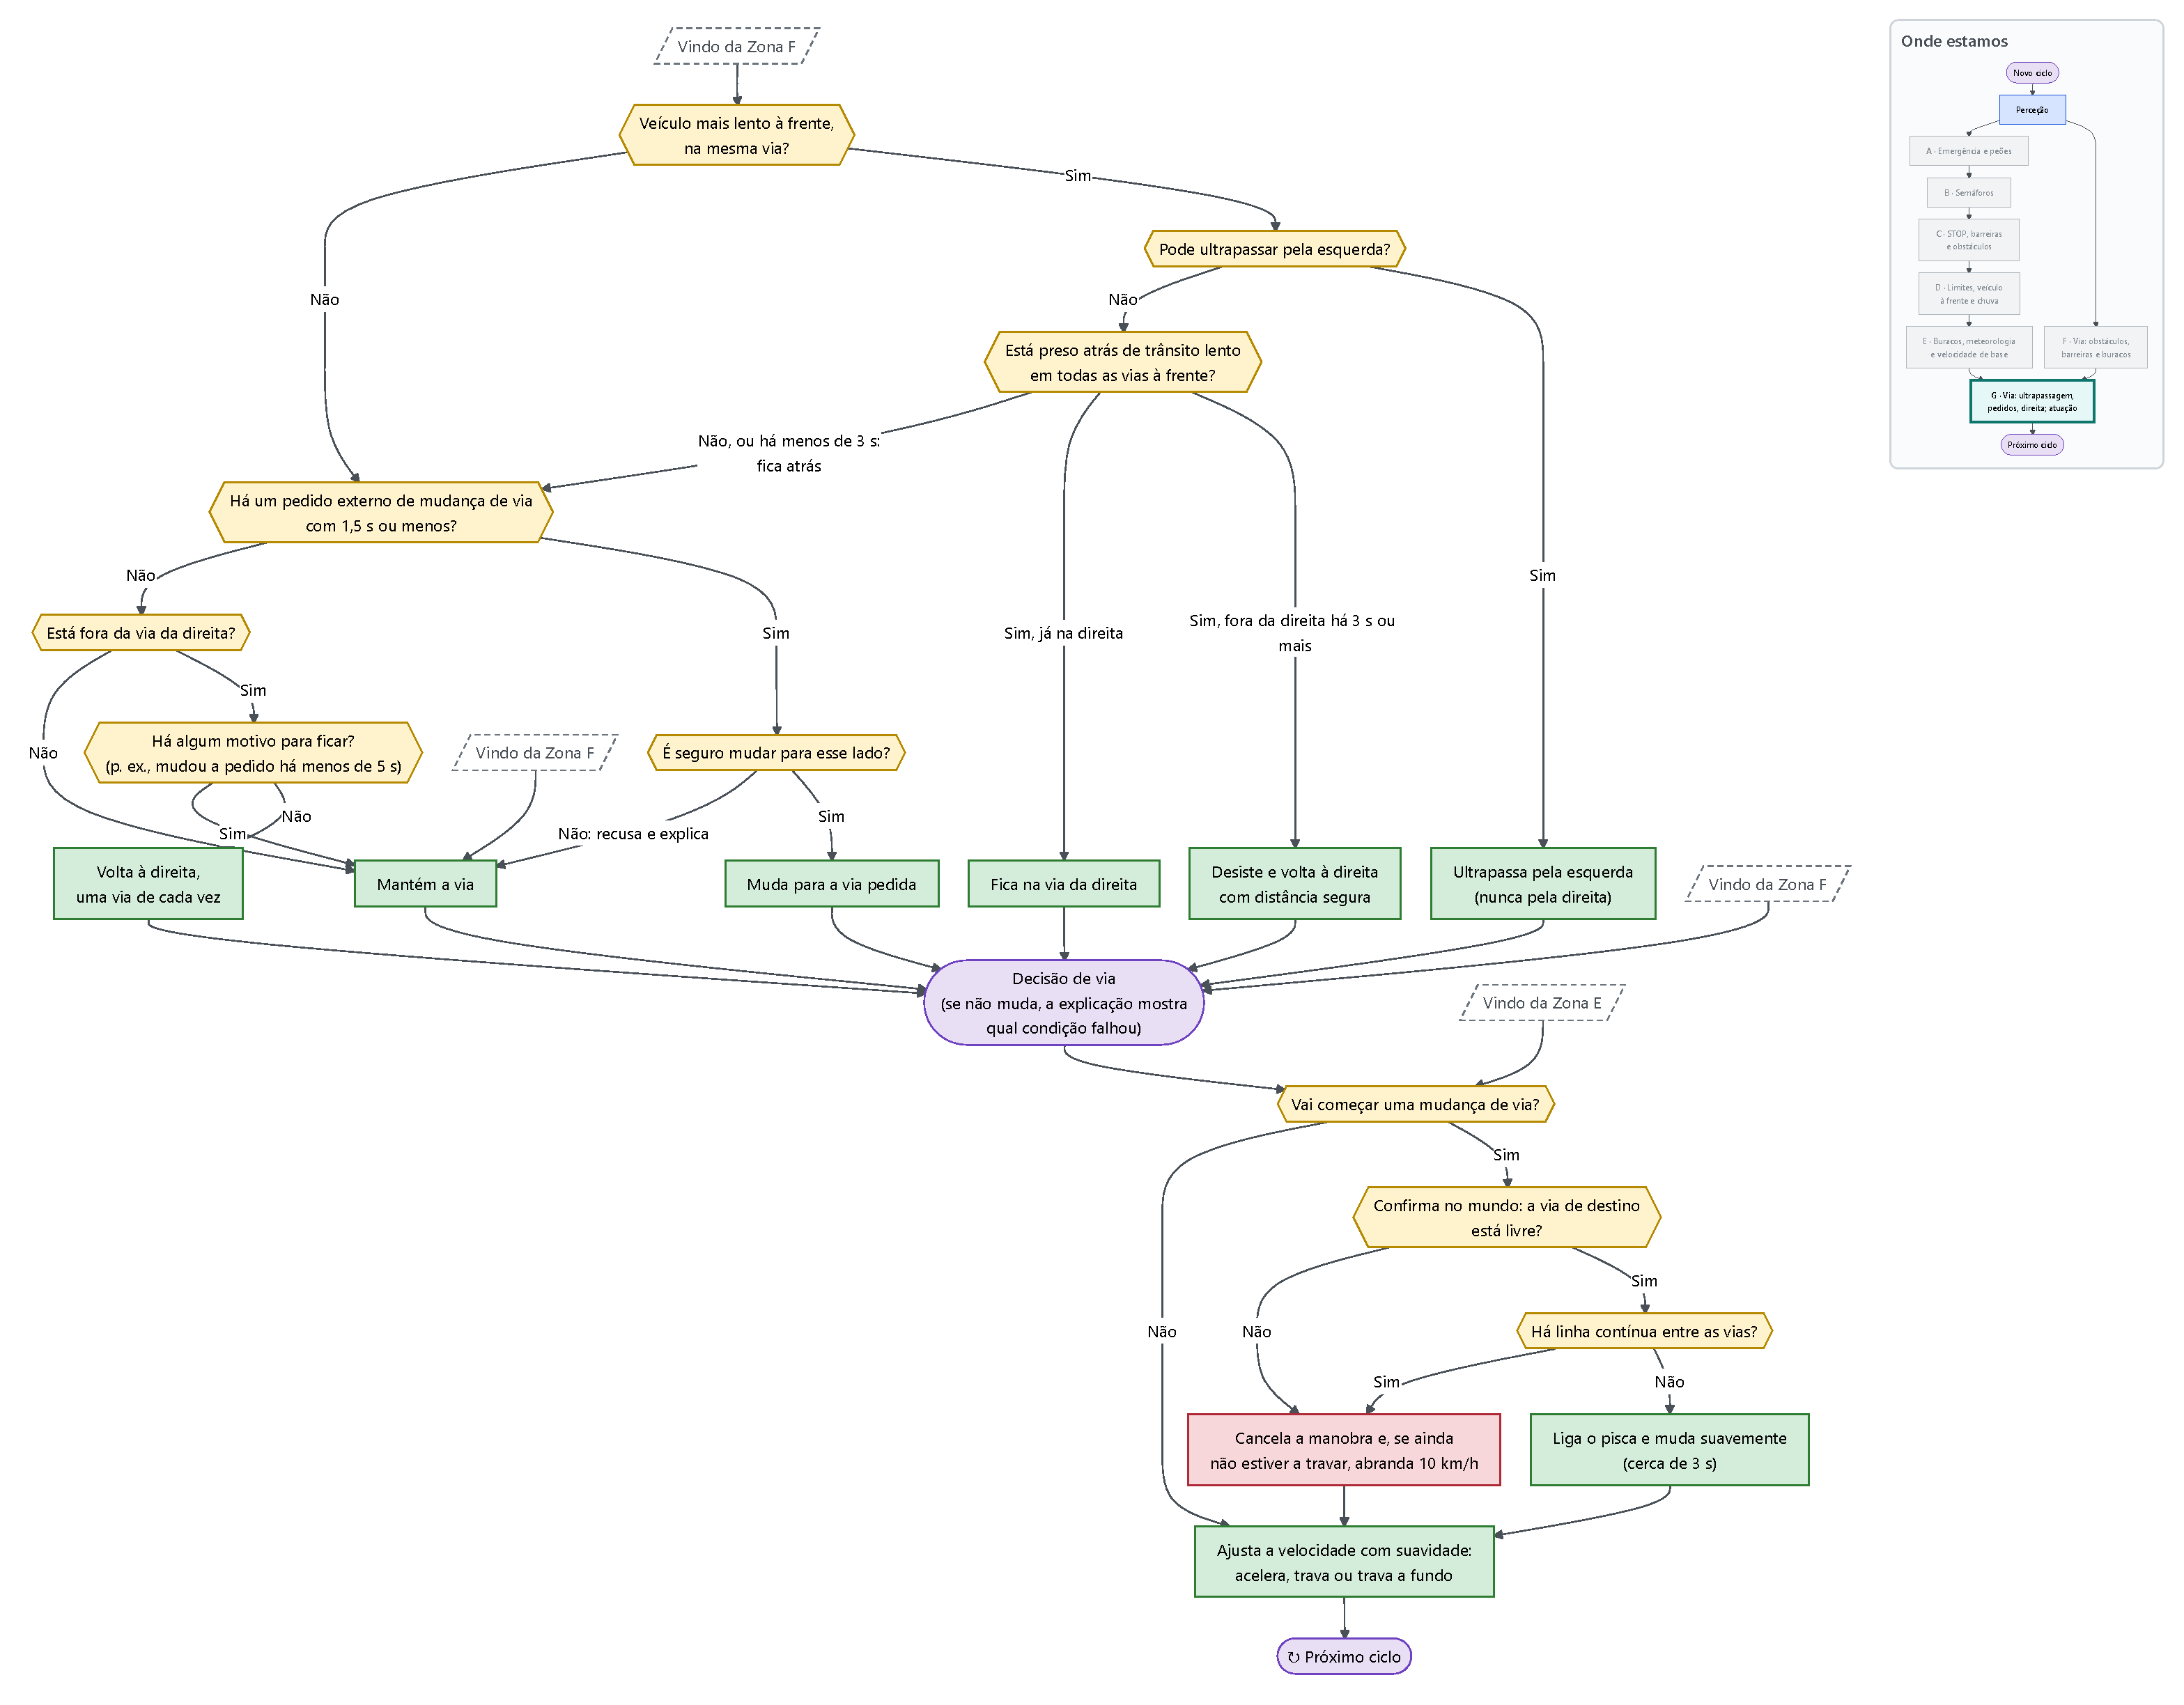
\includegraphics[width=\textheight,height=0.58\textwidth,keepaspectratio]{figuras/fluxograma/zona_G.pdf}
\caption{Zona G: ultrapassagem, pedidos, regresso à direita e atuação}
\label{fig:zonaG}
\end{sidewaysfigure}

\clearpage

\section{Explicação da decisão}\label{sec:explicacao}

Cada decisão pode ser explicada em três dimensões complementares (Figura 15), todas implementadas e visíveis na interface.

\begin{figure}[htbp]
\centering
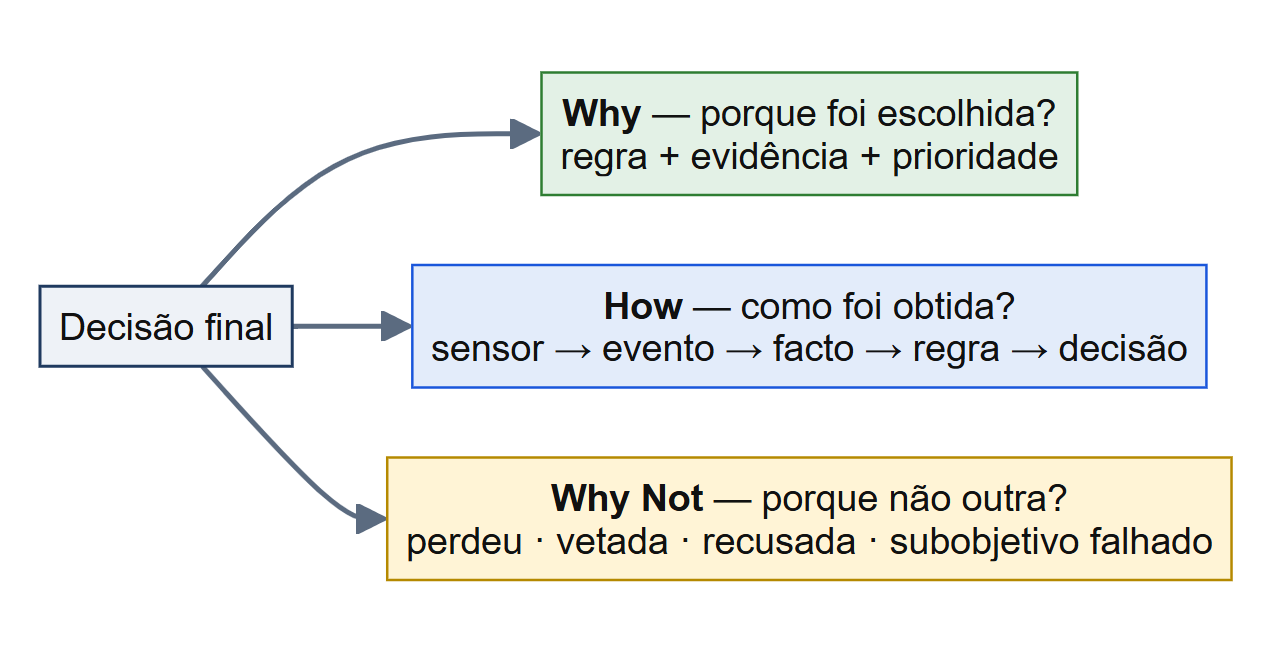
\includegraphics[width=0.62\textwidth]{figuras/explicacao.png}
\caption{Três dimensões de explicação}
\label{fig:explicacao}
\end{figure}

\begin{itemize}
  \item \textbf{\ing{Why}.} A decisão guarda, por canal, a regra que a originou, a razão, a
        evidência (os valores dos factos usados), o risco e a prioridade.
  \item \emph{\textbf{How}}. A linha temporal regista, com instante, cada inserção, atualização e remoção de factos e cada regra disparada, o que permite reconstruir o percurso sensor → evento → facto → regra → decisão. O inspetor da memória de trabalho mostra os factos ativos e, na explicação da viagem, o How percorre as perguntas das Figuras 5 e 6 e mostra o ramo seguido em cada uma.
  \item \textbf{\ing{Why Not}.} Todas as propostas do ciclo ficam guardadas com o seu destino:
        venceu, perdeu para outra (\cod{LOST\_TO}), foi anulada por uma paragem ou emergência
        (\cod{VETOED\_BY}), teve a velocidade limitada por um teto (\cod{CAPPED}) ou foi recusada
        pelo atuador (\cod{REJECTED\_BY}). Quando uma mudança de via nem chega a ser proposta, o
        sistema mostra qual dos subobjetivos de segurança falhou (manobra em curso, linha
        contínua, via ocupada ou falta de espaço para seguir o veículo da frente).
\end{itemize}

Como recomendou o perito, as explicações são o resultado das próprias regras: o texto apresentado
é a razão e a evidência registadas pela regra que disparou, e não uma descrição escrita à parte. Ao
terminar uma viagem (STOP), a sessão é gravada em JSON e cada decisão pode ser questionada depois, a
partir do ciclo gravado, sem reavaliar nada.

O capítulo seguinte mostra como este processo está implementado e como pode ser acompanhado em
tempo real.

% ---------------------------------------------------------------
% 6. Implementação
% ---------------------------------------------------------------
\chapter{Implementação}\label{cap:implementacao}

\section{Arquitetura}\label{sec:arquitetura}

A arquitetura utilizada separa o mundo simulado, a perceção e o conhecimento (Figura 16). O WorldState contém tudo o que existe no cenário, mas o motor de inferência só conhece o que os sensores detetaram. Toda a política de decisão está nas regras; o código Java simula, encaminha eventos e aplica decisões, e a interface apenas apresenta e envia comandos. A Tabela 8 apresenta os principais componentes, com base em dois princípios:

\begin{itemize}
  \item \textbf{A cada} 100 ms é executado um ciclo; todos os pedidos REST passam por métodos sincronizados do SimulationEngine
  \item \textbf{Comandos por REST, estado por \ing{WebSocket}.} Cada comando tem a sua resposta; o
        estado completo é enviado para o \ing{browser} a cada ciclo.
\end{itemize}

\begin{figure}[htbp]
\centering
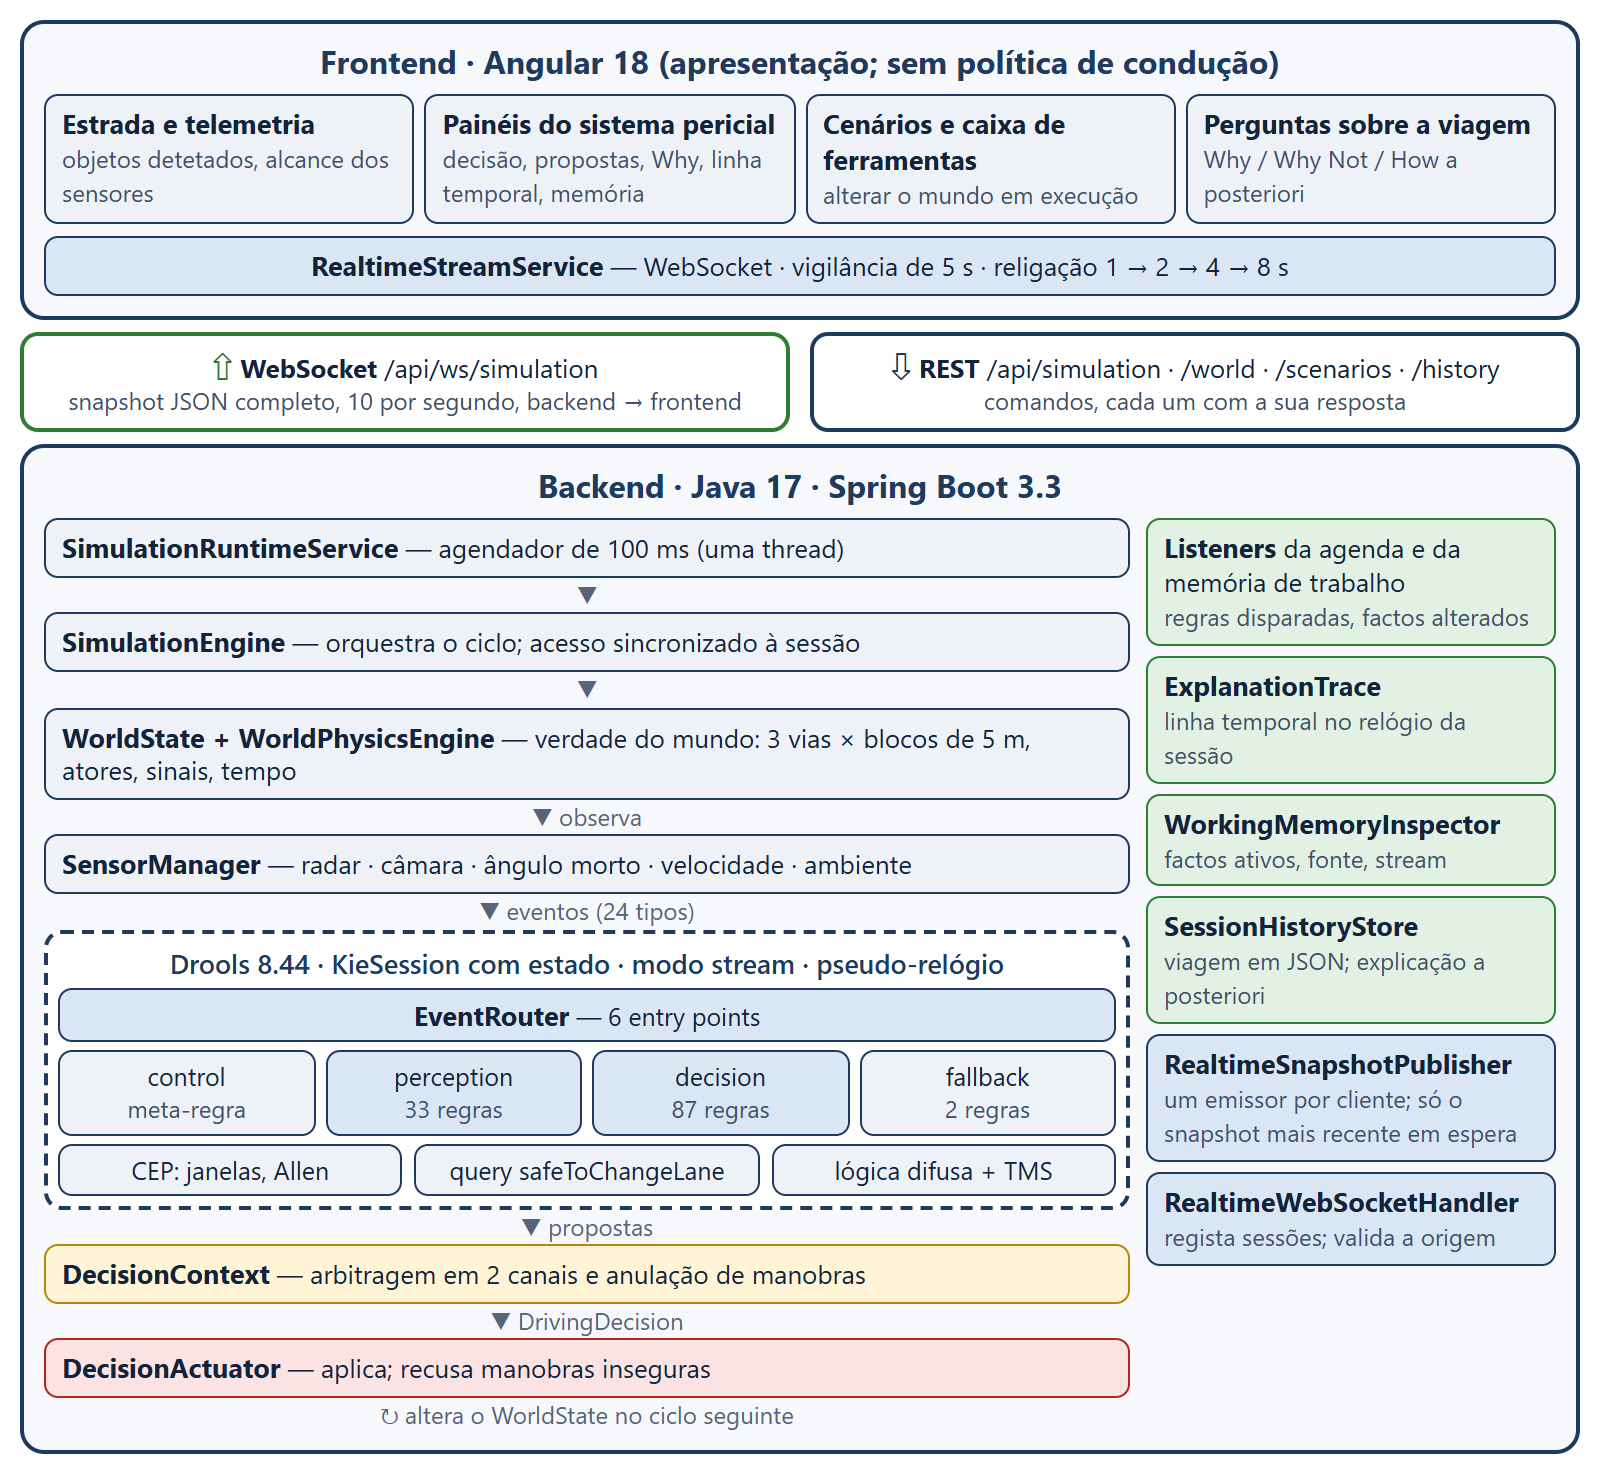
\includegraphics[width=0.92\textwidth,height=0.62\textheight,keepaspectratio]{figuras/arquitetura.png}
\caption{Arquitetura do sistema e fluxo de informação}
\label{fig:arquitetura}
\end{figure}

\begin{table}[htbp]
\centering
\small
\caption{Componentes principais}\label{tab:componentes}
\rowcolors{2}{white}{corFundo}
\begin{tabular}{@{}L{0.33\textwidth}L{0.61\textwidth}@{}}
\linhacab \cab{Componente} & \cab{Responsabilidade} \\
\cod{SimulationRuntimeService} & Agendador de 100 ms; constrói o \ing{snapshot} de cada ciclo e entrega-o ao publicador \\
\cod{SimulationEngine} & Responsável pelo ciclo; arranque, pausa, paragem, cenários e alterações ao mundo \\
\cod{WorldState} · \cod{WorldPhysicsEngine} & Mundo simulado (estrada em matriz, veículos, peões, sinais, tempo) e a sua evolução física \\
\cod{SensorManager} & Os cinco sensores, cada um com cadência e alcance próprios \\
\cod{EventRouter} · \cod{KnowledgeSession} & Encaminham os eventos para os \ing{entry points} e gerem a \cod{KieSession} \\
\cod{DecisionContext} & Recolhe as propostas do ciclo e arbitra-as por canal, registando o destino de cada uma \\
\cod{DecisionActuator} & Aplica a decisão (aceleração, pisca, mudança de via) e recusa manobras inseguras \\
\cod{ExplanationTrace} · \ing{listeners} & Linha temporal das regras e dos factos; inspetor da memória de trabalho \\
\cod{SessionHistoryStore} & Grava cada viagem em JSON e responde a \ing{Why}, \ing{Why Not} e \ing{How} a posteriori \\
\cod{RealtimeSnapshotPublisher} & Envia o \ing{snapshot} a cada \ing{browser} ligado, sem nunca bloquear a simulação \\
\end{tabular}
\end{table}

\begin{table}[htbp]
\centering
\small
\caption{Tecnologias utilizadas}\label{tab:tecnologias}
\rowcolors{2}{white}{corFundo}
\begin{tabular}{@{}L{0.17\textwidth}L{0.29\textwidth}L{0.48\textwidth}@{}}
\linhacab \cab{Componente} & \cab{Tecnologia} & \cab{Utilização} \\
\ing{Backend} & Java 17, Spring Boot 3.3.4 & Simulação, sensores, motor de inferência e API REST/\ing{WebSocket} \\
Motor de regras & \ing{Drools} / KIE 8.44 & Sessão com estado, regras DRL, CEP, encadeamento progressivo e consultas \\
\ing{Frontend} & Angular 18, RxJS & Visualização da simulação e dos painéis do sistema pericial \\
Comunicação & \ing{WebSocket} e REST & Estado em tempo real (\ing{WebSocket}) e comandos (REST) \\
Testes & JUnit 5, Jasmine/Karma, Playwright & Regras, arbitragem, ciclo de simulação, integração e testes de ponta a ponta \\
\end{tabular}
\end{table}

\FloatBarrier
\section{O ciclo de 100 ms}\label{sec:ciclo}

A Figura 17, a título de exemplo, mostra, por ordem, o que acontece em cada ciclo.

\begin{figure}[htbp]
\centering
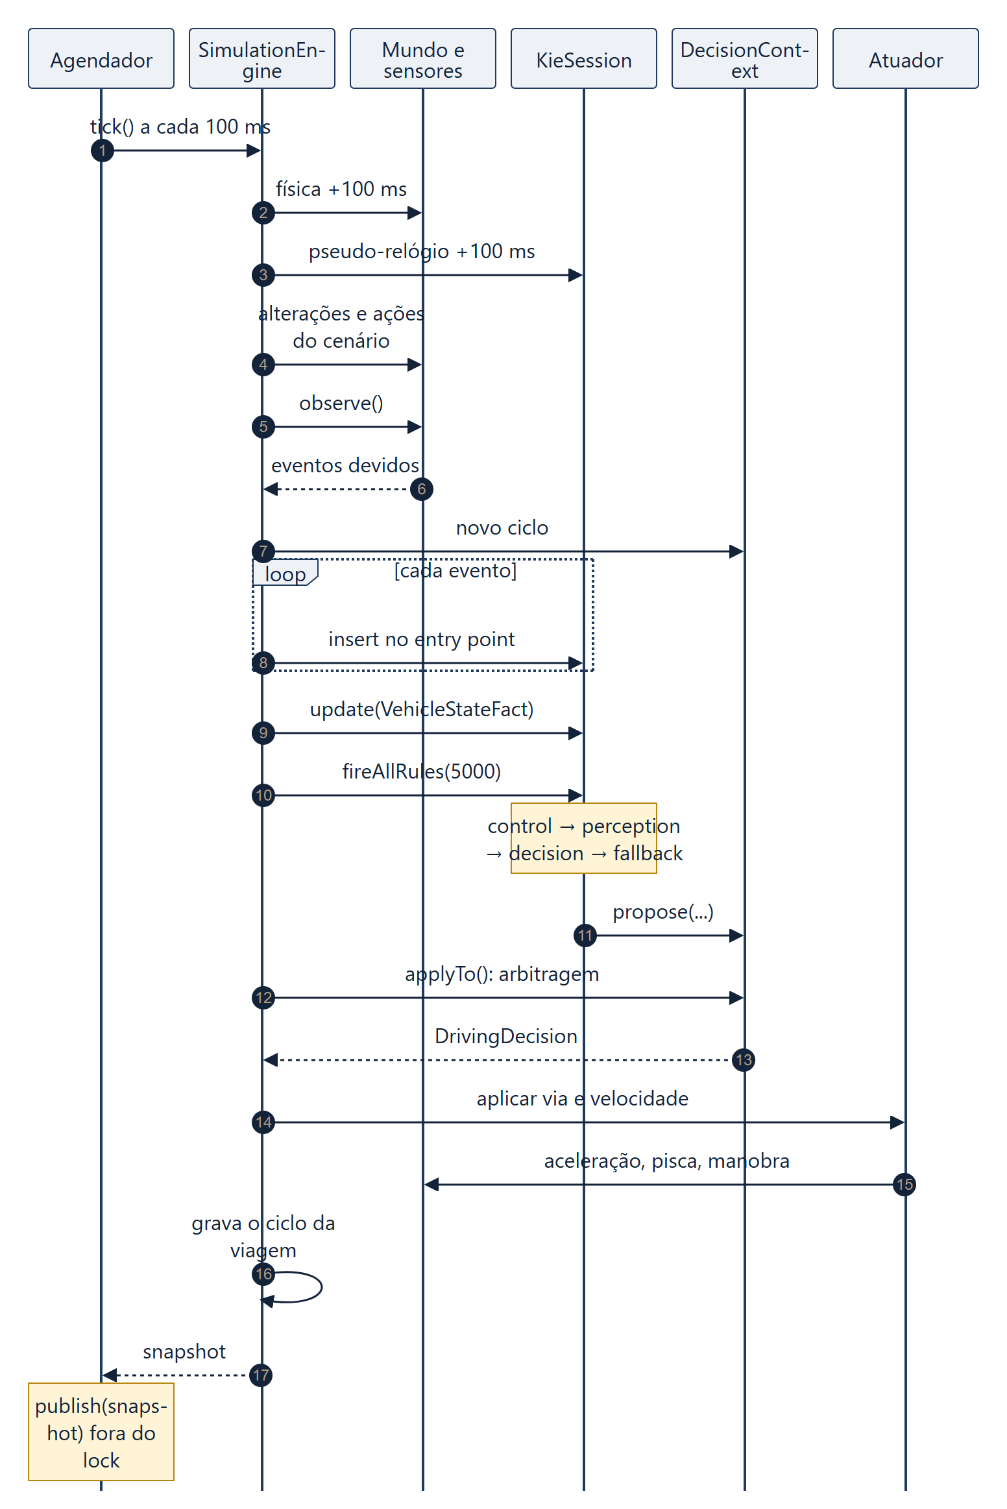
\includegraphics[width=\textwidth,height=0.80\textheight,keepaspectratio]{figuras/ciclo_simulacao.png}
\caption{Sequência de um ciclo de simulação}
\label{fig:ciclo-simulacao}
\end{figure}

\FloatBarrier
\section{O motor de inferência}\label{sec:motor}

\textbf{Entry points.} Os eventos entram por seis fluxos com nome (Tabela 10), o que separa semanticamente a origem da informação e permite às regras temporais ler só o fluxo de que precisam.

\begin{table}[htbp]
\centering
\small
\caption{\ing{Entry points} e eventos encaminhados}\label{tab:entrypoints}
\rowcolors{2}{white}{corFundo}
\begin{tabular}{@{}L{0.30\textwidth}L{0.64\textwidth}@{}}
\linhacab \cab{\ing{Entry point}} & \cab{Eventos} \\
\cod{VEHICLE\_STREAM} & Velocidade do veículo \\
\cod{PERCEPTION\_STREAM} & Distância, velocidade relativa e TTC; peões; ocupação das vias laterais; veículos nas vias vizinhas \\
\cod{ROAD\_STREAM} & Sinais de limite e de STOP, passadeiras, buracos, obstáculos, barreiras \\
\cod{TRAFFIC\_STREAM} & Estado dos semáforos \\
\cod{ENVIRONMENT\_STREAM} & Chuva, visibilidade e aderência \\
\cod{COMMAND\_STREAM} & Pedidos de aceleração e de mudança de via \\
\end{tabular}
\end{table}

Metaconhecimento de controlo. As regras encontram-se organizadas em grupos (Tabela 11), cuja execução é controlada por uma meta-regra.

\begin{table}[htbp]
\centering
\small
\caption{Grupos de agenda}\label{tab:grupos}
\rowcolors{2}{white}{corFundo}
\begin{tabular}{@{}L{0.16\textwidth}C{0.09\textwidth}L{0.67\textwidth}@{}}
\linhacab \cab{Grupo} & \cab{Regras} & \cab{Função} \\
\cod{control} & 1 & Meta-regra «\ing{Control: perceive, then decide, then fall back}» (saliência 10000) \\
\cod{perception} & 33 & Eventos $\rightarrow$ factos de estado; expiração das perceções; lados seguros para mudar de via \\
\cod{decision} & 87 & Regras que propõem ações e mantêm estados intermédios (lógica difusa, arranque, ultrapassagem) \\
\cod{fallback} & 2 & Manter a velocidade se nada foi proposto; arrancar quando nada retém o veículo \\
\end{tabular}
\end{table}

\textbf{Raciocínio temporal (CEP).} Os 24 tipos de evento são declarados com @role(event), @timestamp e @expires (3 a 30 s), o que mantém a memória limitada.

\textbf{Encadeamento regressivo.} «É seguro mudar de via para este lado?» é um objetivo, definido por uma consulta que se prova a partir de quatro subobjetivos: maneuverIdle, noContinuousLine, sideClear e roomToFollow.


\textbf{Lógica difusa.} A visibilidade e a aderência são vagas, por isso são fuzzificadas em quatro termos (fraca, reduzida, razoável, boa) e combinadas por cinco regras difusas (E = mínimo, OU = máximo) como, por exemplo, com chuva, visibilidade 0,7 e aderência 0,65, o teto obtido é de cerca de 51 km/h. As pertenças e as conclusões difusas são inseridas com insertLogical: quando a leitura meteorológica muda, perdem a justificação e são retiradas pelo próprio motor.

\FloatBarrier
\section{Comunicação em tempo real: \ing{WebSocket}}\label{sec:websocket}

A interface tem de mostrar, dez vezes por segundo, o veículo, as deteções, a decisão dos dois canais, todas as propostas com o seu destino, a linha temporal e a memória de trabalho. Para isso, o backend mantém com cada browser uma ligação WebSocket em /api/ws/simulation e, a cada ciclo, envia por ela um snapshot JSON completo do sistema. A ligação é aberta uma vez e fica aberta: cada atualização é apenas uma frame de texto e chega à interface no próprio ciclo em que a decisão é tomada. O canal é usado num só sentido, do backend para o frontend, e sem protocolos adicionais (sem STOMP). Os comandos (iniciar, parar, carregar cenários, inserir elementos) continuam em REST (Tabela 12), porque cada um precisa da sua própria resposta e do seu código de erro; depois de cada comando, o backend envia logo um snapshot, para que o efeito apareça sem esperar pelo ciclo seguinte.

\begin{table}[htbp]
\centering
\small
\caption{Separação entre comandos (REST) e estado (\ing{WebSocket})}\label{tab:rest}
\rowcolors{2}{white}{corFundo}
\begin{tabular}{@{}L{0.52\textwidth}L{0.42\textwidth}@{}}
\linhacab \cab{Pedido} & \cab{Função} \\
\cod{POST /api/simulation/\{start | pause | resume | stop | reset\}} & Ciclo de vida da simulação \\
\cod{POST /api/scenarios/\{id\}/load} & Carregar um cenário \\
\cod{POST · PUT · DELETE /api/world/elements}, \cod{/api/world/actors} & Inserir, alterar ou remover elementos e atores durante a simulação \\
\cod{PUT /api/world/map/cells} & Pintar uma célula da matriz da estrada \\
\cod{POST /api/environment} & Mudar a meteorologia \\
\cod{GET /api/history/sessions} · \cod{POST \ldots/\{id\}/why} & Viagens gravadas e perguntas \ing{Why} / \ing{Why Not} / \ing{How} \\
\cod{ws://\ldots/api/ws/simulation} & Estado completo a cada ciclo e após cada comando \\
\end{tabular}
\end{table}

\textbf{Formato da mensagem.} Cada frame tem a forma \{"event":"snapshot","payload":\{\ldots\}\} e é serializada pelo mesmo ObjectMapper da API REST, pelo que é exatamente o mesmo JSON de GET /api/simulation/state. A Tabela 13 resume o conteúdo.

\begin{table}[htbp]
\centering
\small
\caption{Conteúdo de um \ing{snapshot}}\label{tab:snapshot}
\rowcolors{2}{white}{corFundo}
\begin{tabular}{@{}L{0.32\textwidth}L{0.62\textwidth}@{}}
\linhacab \cab{Campo} & \cab{Conteúdo} \\
\cod{egoVehicle} · \cod{environment} & Velocidade, posição, via, aceleração, estado da manobra, pisca; chuva, visibilidade e aderência \\
\cod{currentDecision} & Decisão de velocidade e de via, regra, razão, evidência, risco e prioridade; todas as propostas com o seu destino; resposta ao «porque não mudar de via» para cada lado \\
\cod{sensors} · \cod{detectedObjectIds} & Telemetria de cada sensor e os objetos realmente detetados pela câmara e pelo radar \\
\cod{worldObjects} · \cod{roadMap} & Elementos do mundo relativos ao veículo e a matriz da estrada \\
\cod{workingMemory} · \cod{recentTimeline} & Factos ativos (tipo, valor, fonte, \ing{stream}) e as últimas 160 entradas da linha temporal \\
\cod{status} · \cod{simulationTimeMillis} & Estado da simulação e tempo simulado \\
\end{tabular}
\end{table}

A Figura 18 mostra a ligação completa: o handshake, a validação da origem, o snapshot imediato, o envio periódico e a interação com os comandos REST. Como o CORS não se aplica a WebSockets, a origem é verificada no handshake: só a interface do projeto (http://localhost:4200) pode abrir o canal; outra origem recebe 403.

\begin{figure}[htbp]
\centering
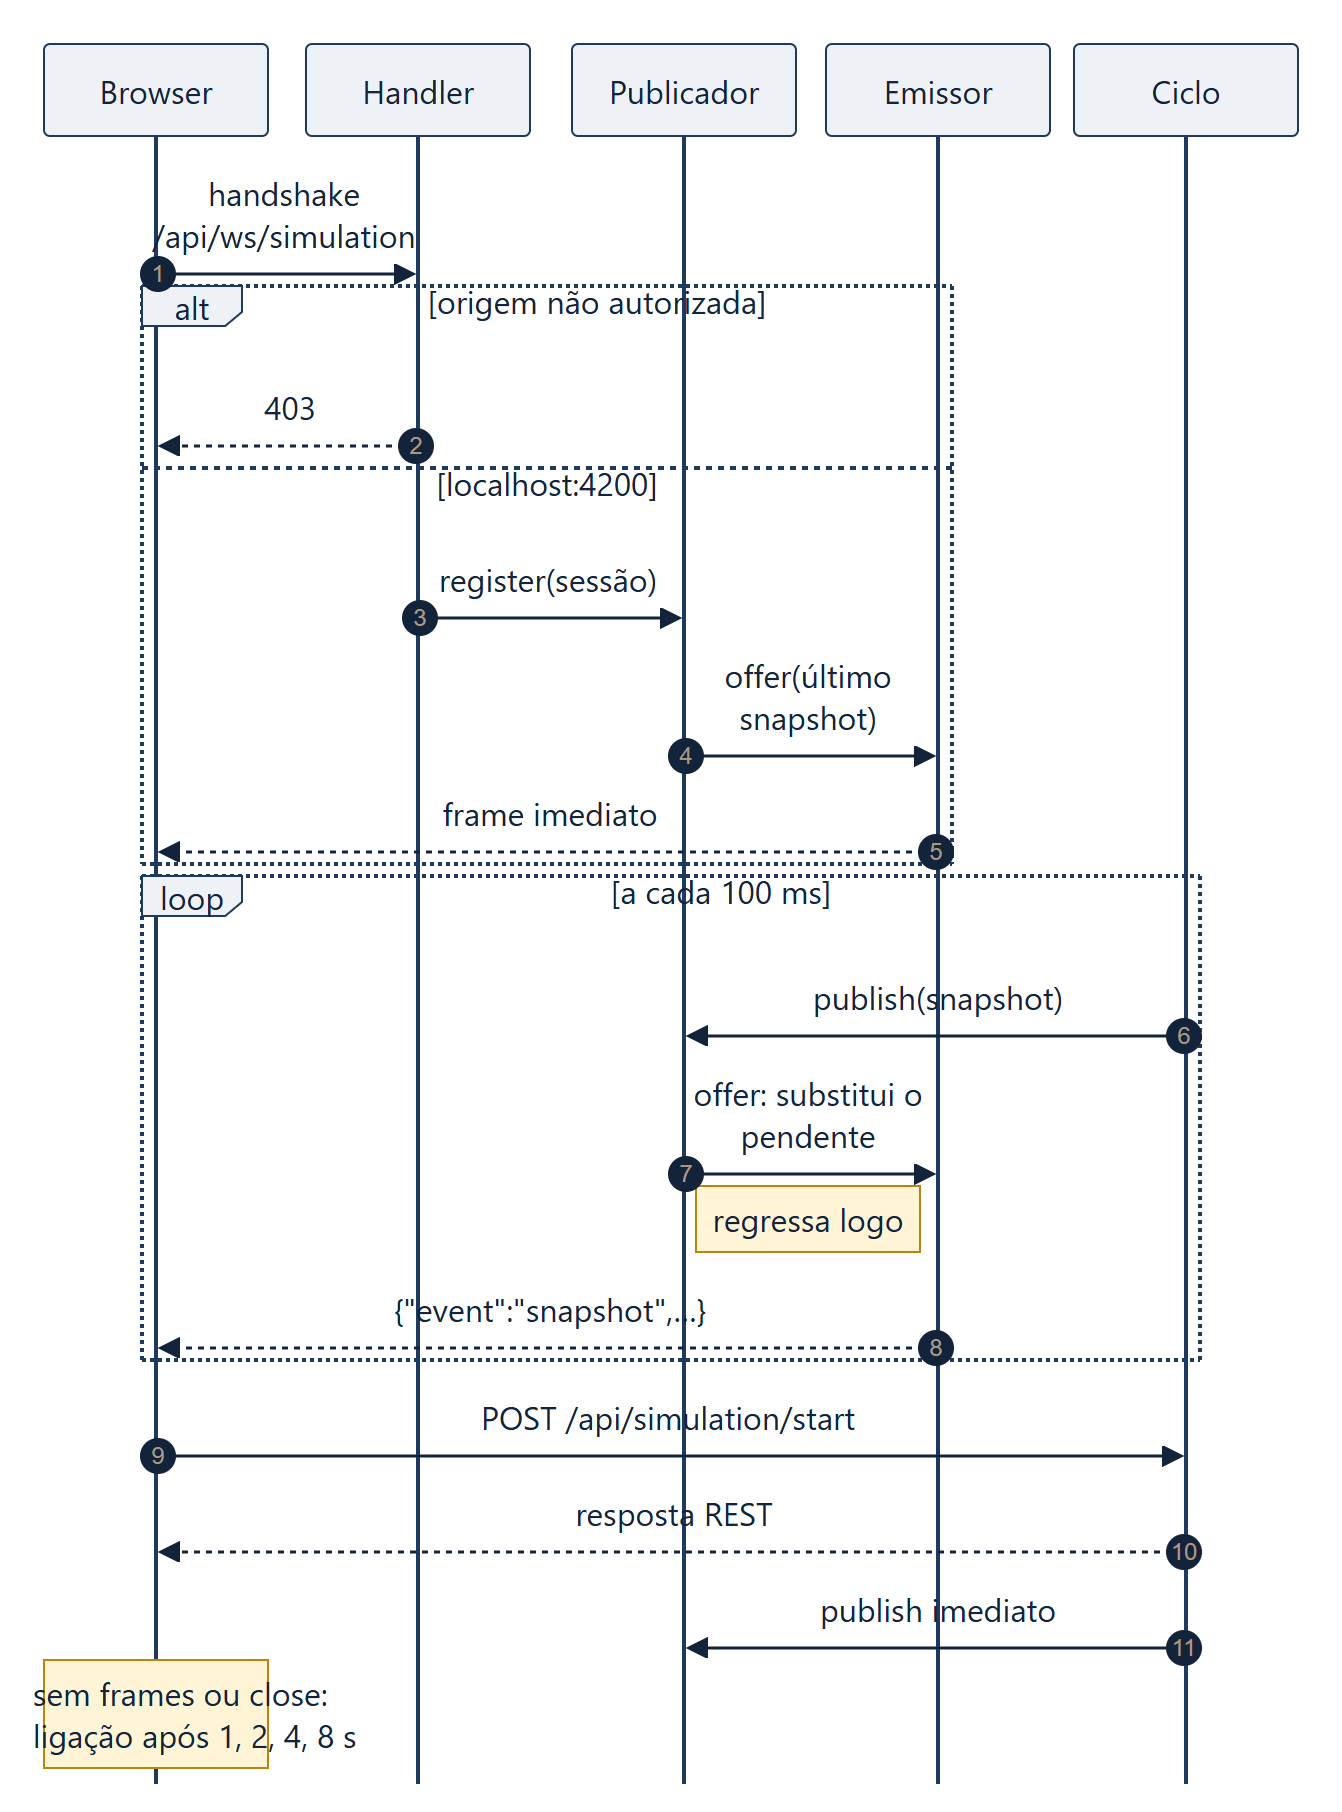
\includegraphics[width=\textwidth,height=0.78\textheight,keepaspectratio]{figuras/websocket_sequencia.png}
\caption{Sequência da ligação \ing{WebSocket} e da sua interação com os comandos REST}
\label{fig:ws-sequencia}
\end{figure}

A implementação resolve três problemas de um canal de tempo real:

\begin{itemize}
  \item \textbf{Um cliente lento não atrasa a simulação.} A publicação nunca espera pelo envio: cada navegador tem o seu emissor, com no máximo uma escrita em curso e apenas o snapshot mais recente em espera. Um separador em segundo plano perde frames intermédios, mas como cada snapshot é um estado completo não perde informação.
  \item \textbf{Entrada imediata.} Quem liga, ou volta a ligar, recebe logo o último snapshot, sem esperar pelo ciclo seguinte.
  \item \textbf{Recuperação automática.} O frontend considera a ligação morta se não receber frames durante 5 s e volta a ligar com esperas crescentes (1 s, 2 s, 4 s, até 8 s). A ligação valida a origem do pedido, para que só a interface do projeto a possa abrir.
\end{itemize}

Os três problemas são resolvidos em dois lados: no servidor, que nunca pode ficar à espera de um
\ing{browser}, e no cliente, que tem de perceber sozinho quando a ligação morreu.

\textbf{Servidor: um emissor por cliente.} Uma escrita bloqueante num socket de um browser lento (por exemplo, um separador em segundo plano) pararia o fio da simulação. Por isso, o RealtimeSnapshotPublisher dá a cada sessão o seu próprio emissor (Figura 19):

\begin{itemize}
  \item \cod{publish()} guarda o \ing{snapshot} e entrega-o a cada emissor; regressa de imediato e
        é chamado fora do \ing{lock} da simulação, pelo que os pedidos REST também nunca esperam
        pela rede;
  \item cada emissor tem uma só posição de espera (AtomicReference) e no máximo uma escrita em curso (AtomicBoolean): um snapshot novo substitui o que ainda não foi enviado. Um cliente lento perde frames intermédias, mas como cada frame é um estado completo nunca fica com informação errada;
  \item as escritas correm em \ing{threads} próprias (\cod{ws-sender}), o que também garante que
        uma \cod{WebSocketSession}, que não é segura entre \ing{threads}, recebe uma escrita de
        cada vez;
  \item o registo de um cliente novo e a publicação partilham um lock, pelo que nenhum cliente perde nem recebe fora de ordem um snapshot concorrente;
  \item se uma escrita falhar ou expirar, o cliente é removido e a sessão fechada; um erro de
        serialização descarta apenas essa \ing{frame}.
\end{itemize}

\begin{figure}[htbp]
\centering
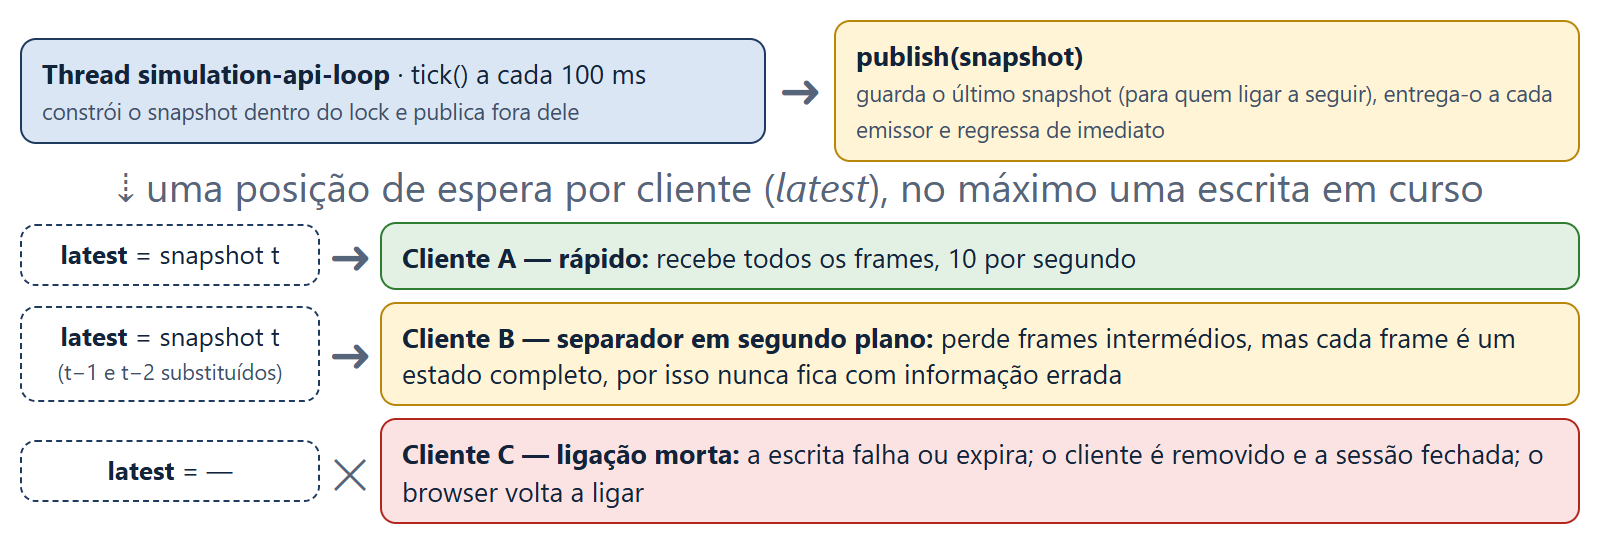
\includegraphics[width=\textwidth]{figuras/websocket_publicador.png}
\caption{Publicação sem bloqueio: um emissor e uma posição de espera por cliente}
\label{fig:ws-publicador}
\end{figure}

\textbf{Cliente: deteção de falhas e religação.} No Angular, o RealtimeStreamService abre o socket fora da zona do Angular, para que só um snapshot dispare deteção de alterações. Uma ligação é dada como perdida quando fecha, quando chega uma frame que não é JSON ou quando passam 5 s sem frames --- como o backend envia um snapshot a cada ciclo, mesmo parado, este silêncio só acontece se a ligação morreu sem aviso (suspensão do portátil, mudança de rede). O SimulationStateService volta então a ligar com esperas crescentes de 1, 2, 4 e 8 s (Figura 20), mostra o estado do canal (LIVE ou RECONNECTING) e um aviso; o primeiro snapshot repõe tudo.

\begin{figure}[htbp]
\centering
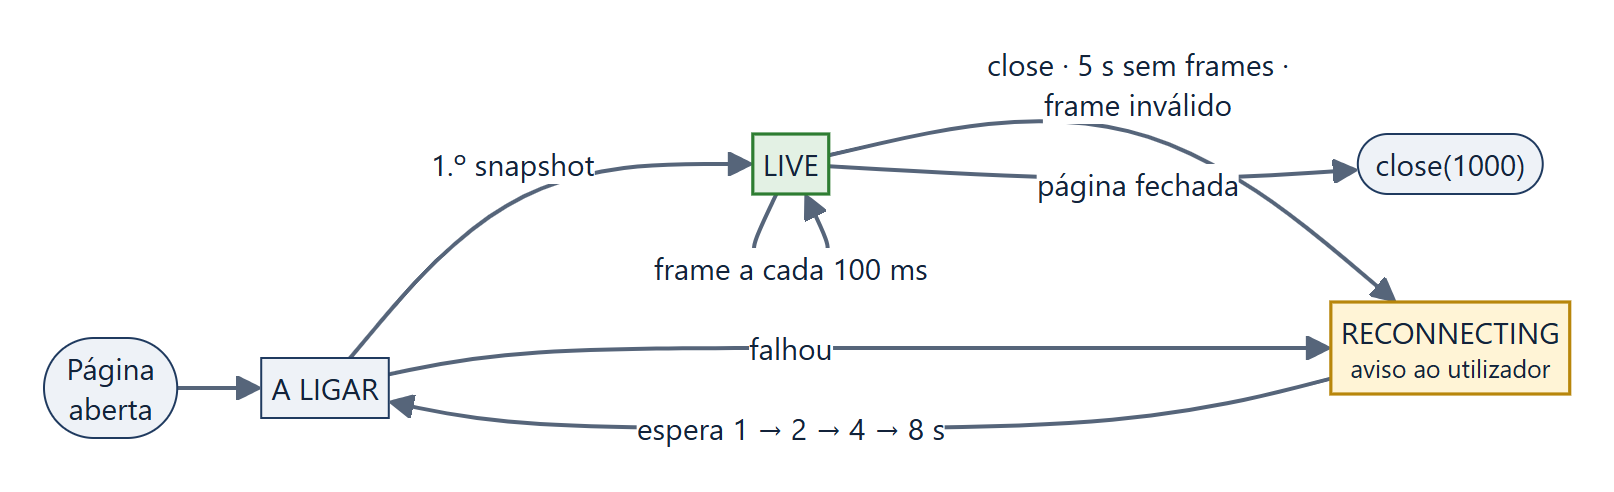
\includegraphics[width=\textwidth]{figuras/websocket_estados.png}
\caption{Estados do canal no \ing{browser}}
\label{fig:ws-estados}
\end{figure}

\paragraph{Desempenho medido.} Com a aplicação a correr e um cliente ligado durante 25 s, chegaram
251 \ing{frames} (10,0 por segundo), com um intervalo médio de 99,8 ms entre \ing{frames}
(desvio-padrão de 11,5 ms) e 33 a 35 KB por \ing{frame}.

\paragraph{Testes do canal.} O publicador tem testes que confirmam que um cliente bloqueado não
atrasa os outros nem a simulação, que um cliente cuja escrita falha é removido e que um cliente
novo recebe logo o último \ing{snapshot}. Um teste de ponta a ponta arranca o servidor real e um
cliente \ing{WebSocket} real e verifica que a travagem de emergência do cenário S8 chega ao cliente
no ciclo em que é inferida, que um cliente religado retoma de imediato e que uma origem estranha é
recusada. No \ing{browser}, os testes Playwright confirmam que a interface se atualiza pelo
\ing{WebSocket} e que recupera sozinha de uma ligação perdida.

Em síntese, o \ing{WebSocket} é o que torna o sistema pericial observável: cada decisão inferida
pelo \ing{Drools} chega à interface no mesmo ciclo, com todas as propostas e a sua explicação, sem
que um \ing{browser} lento ou uma ligação perdida afetem a simulação.

\FloatBarrier
\section{Cenários}\label{sec:cenarios}

Um cenário define o percurso, os atores e as ações temporizadas (por exemplo, mudar o tempo ou pedir uma mudança de via a meio da simulação). Carregar um cenário não dá ao motor acesso ao que nele existe: cada elemento só influencia a decisão depois de detetado. Estão definidos 14 cenários (Tabela 14).

\begin{table}[htbp]
\centering
\small
\caption{Cenários definidos e conhecimento exercitado}\label{tab:cenarios}
\rowcolors{2}{white}{corFundo}
\begin{tabular}{@{}L{0.36\textwidth}L{0.58\textwidth}@{}}
\linhacab \cab{Cenário} & \cab{Conhecimento} \\
S1 Estrada livre & Decisão de base e velocidade de cruzeiro \\
S2 Limite de 90 para 50 km/h & Leitura de sinais e abrandamento a tempo de chegar ao limite \\
S3 Semáforo vermelho & Paragem obrigatória pela distância de travagem; arranque no verde \\
S4 Sinal STOP & Paragem completa de 1,2 s (temporal) e arranque \\
S5 Buraco na via & Desvio para o lado seguro ou redução de velocidade \\
S6 Barreira fechada & Desvio ou paragem antes da barreira \\
S7 Peão a atravessar & Curvas de travagem, paragem e emergência \\
S8 TTC crítico & Janelas temporais (CEP) e travagem de emergência \\
S9 Mudança de via impedida & Encadeamento regressivo e \ing{Why Not} \\
S10 Chuva e baixa aderência & Lógica difusa \\
S11 Cenário sequencial & Várias situações no mesmo percurso \\
S12 Demonstração completa & Percurso de apresentação com ações temporizadas \\
S13 Percurso em matriz & Obstáculos definidos na matriz de vias \\
S14 Ultrapassagem & Ultrapassar um veículo lento e regressar à direita \\
\end{tabular}
\end{table}

Foram escolhidos dois cenários a título de exemplo por serem diferentes entre si e, em conjunto, percorrerem um pouco de todo o sistema: regras normativas e heurísticas, raciocínio temporal, lógica difusa, encadeamento regressivo e os dois canais (velocidade e via). Cada figura mostra a traçagem desde o sensor até à decisão e à explicação.

\subsection{Peão a atravessar (S7)}\label{sec:s7}

O veículo circula a 60 km/h na via central e um peão começa a atravessar 95 m à frente.

\begin{figure}[htbp]
\centering
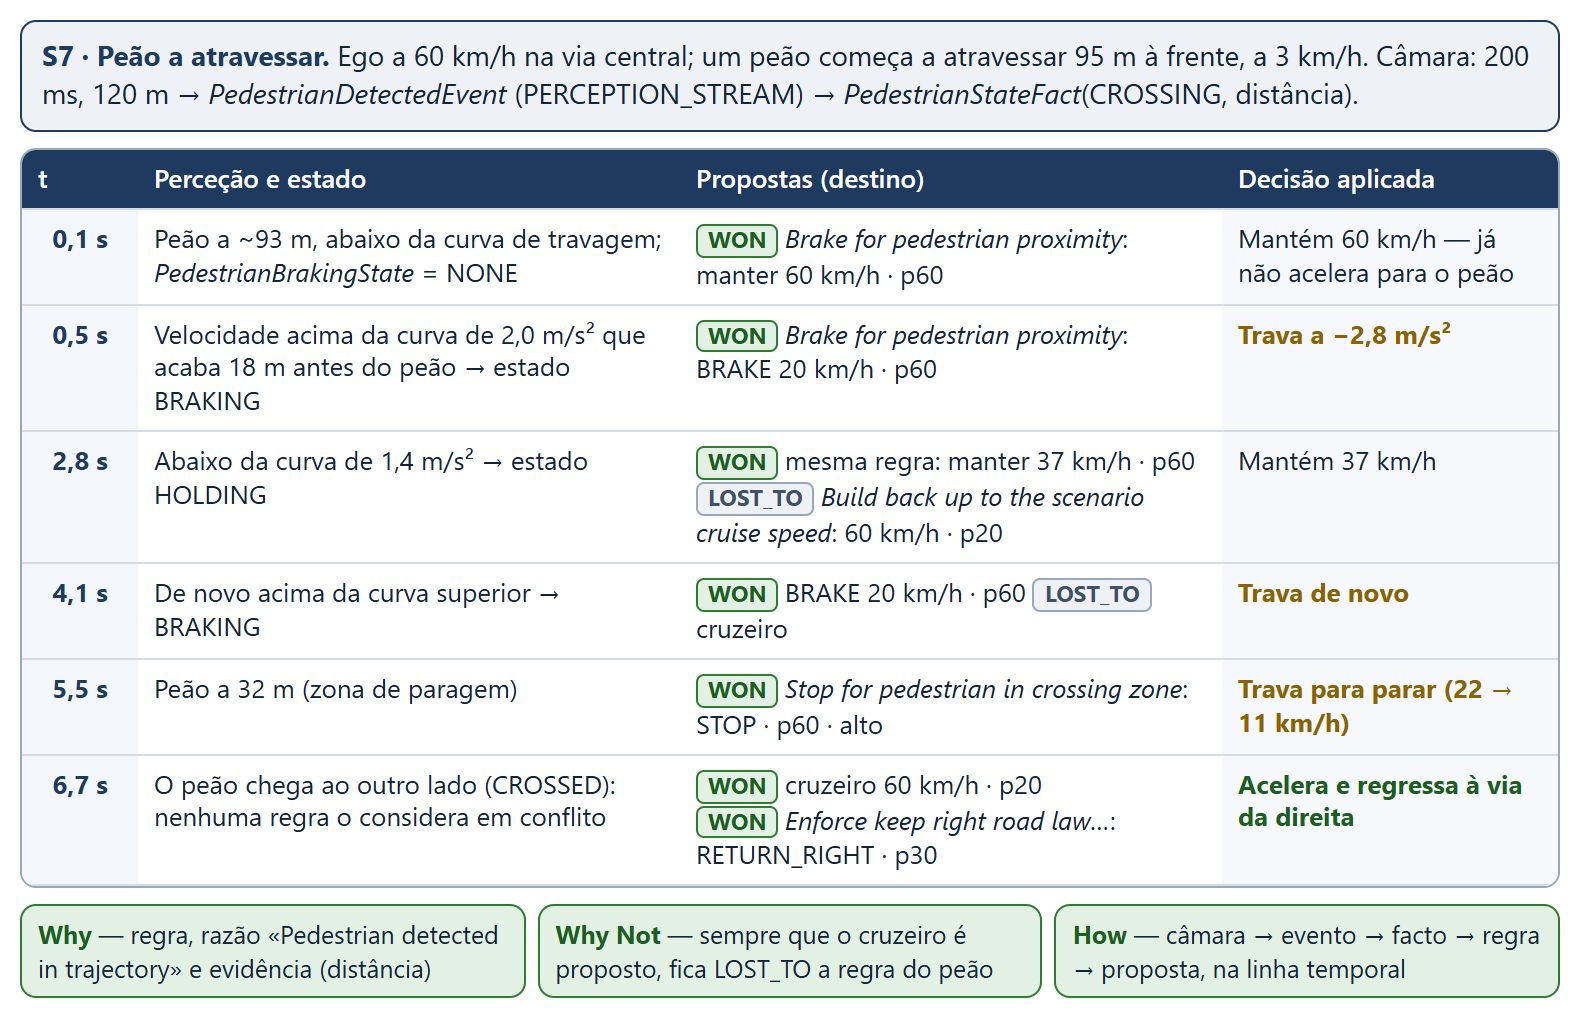
\includegraphics[width=\textwidth]{figuras/tracagem_S7.png}
\caption{Traçagem do cenário S7 --- peão a atravessar}
\label{fig:S7}
\end{figure}

\noindent \textbf{O que demonstra:} conhecimento normativo (ceder passagem) e heurístico (curvas de travagem calculadas, como pediu o perito), estado entre ciclos (PedestrianBrakingState), arbitragem por prioridade e Why com evidência.

\subsection{TTC crítico com chuva (S8)}\label{sec:s8}

O veículo segue a 95 km/h na via central, com outro a 30 km/h 40 m à frente (TTC ≈ 2,2 s); a chuva foi ligada na caixa de ferramentas antes do arranque.

\begin{figure}[htbp]
\centering
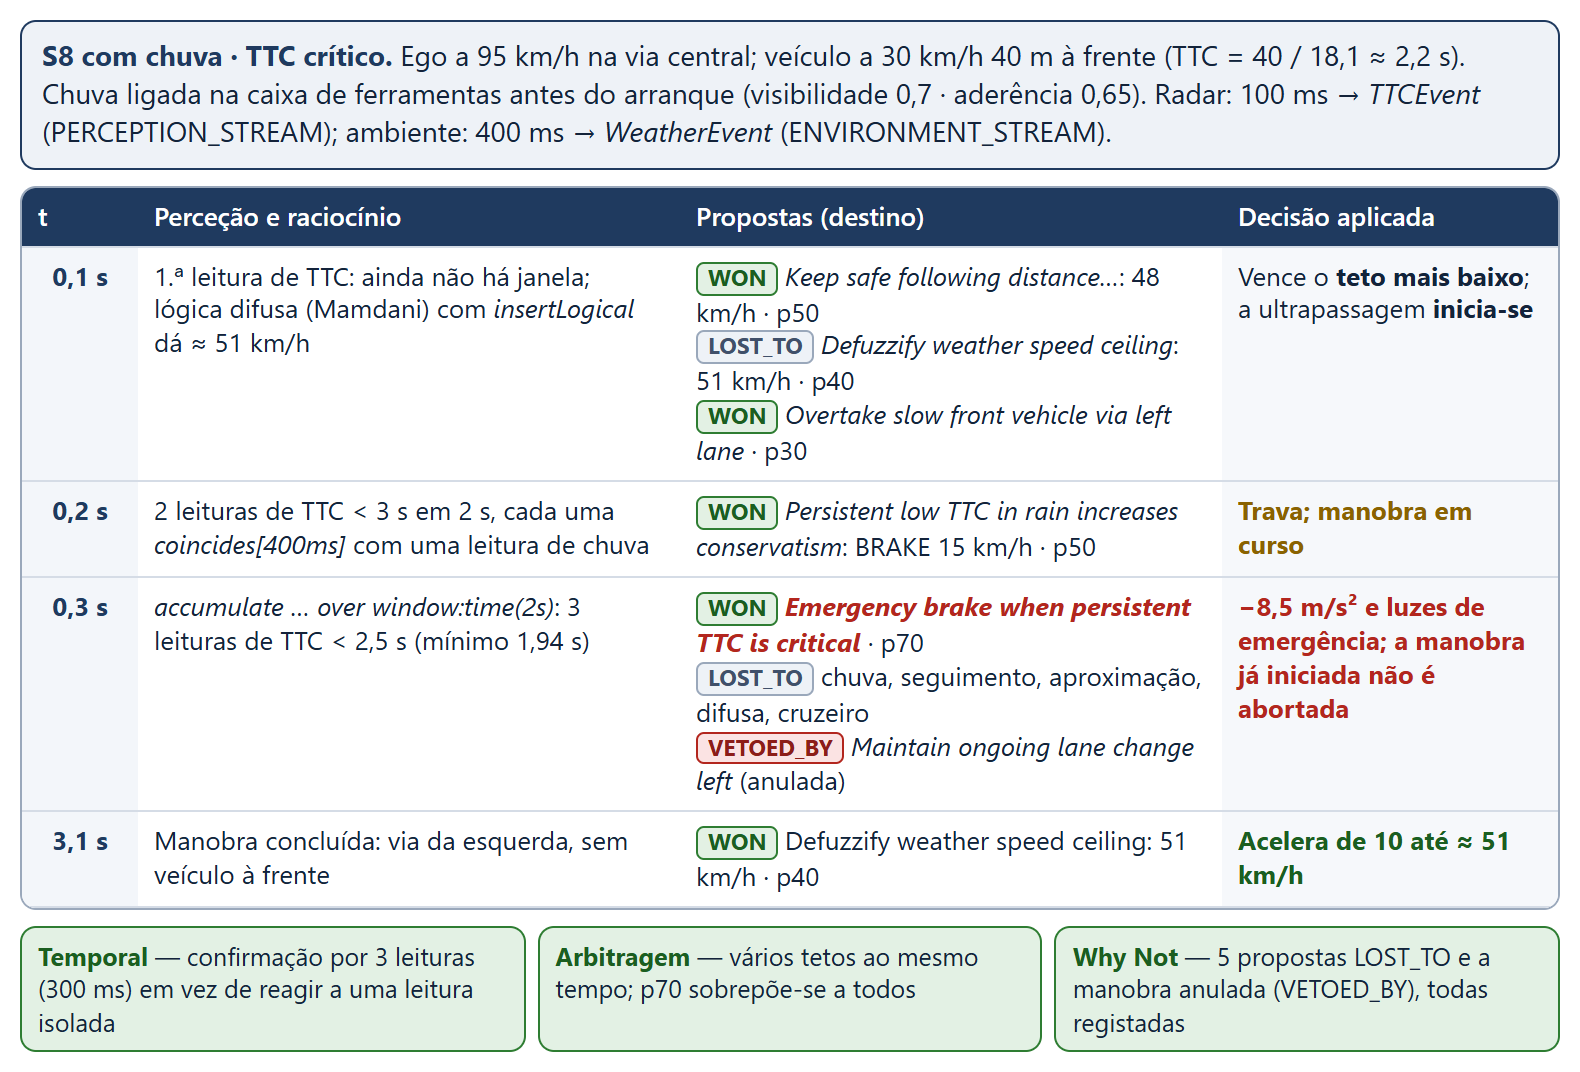
\includegraphics[width=\textwidth]{figuras/tracagem_S8.png}
\caption{Traçagem do cenário S8 com chuva --- TTC crítico, CEP e lógica difusa}
\label{fig:S8}
\end{figure}

\noindent \textbf{O que demonstra:} raciocínio temporal com confirmação adaptada à criticidade, lógica difusa com manutenção da verdade, vários tetos cumpridos em simultâneo e a anulação de uma manobra pelo canal de velocidade.

\FloatBarrier
\section{Testes}\label{sec:testes}

O comportamento foi validado com os cenários anteriores e com testes automáticos com o objetivo de verificar se a decisão respeita as prioridades, que os conflitos têm o vencedor esperado e que situações iguais produzem decisões iguais. Como critérios de aceitação foram usados:

\begin{itemize}
  \item os factos na memória de trabalho que correspondem ao que os sensores detetaram;
  \item a decisão respeita as prioridades e, em conflito, vence a alternativa esperada;
  \item o sistema acompanha a evolução do cenário ao longo do tempo;
  \item cada decisão é explicável pela regra e pela evidência que lhe deram origem;
  \item situações iguais produzem decisões iguais, em execuções repetidas.
\end{itemize}

Validado o comportamento, o capítulo seguinte discute para quem este sistema é útil, o que ainda o
limita e como pode evoluir.

% ---------------------------------------------------------------
% 7. Adequação ao meio envolvente e desenvolvimento futuro
% ---------------------------------------------------------------
\chapter{Adequação ao meio envolvente e desenvolvimento futuro}\label{cap:adequacao}

\section{Adequação a empresas e organizações}\label{sec:empresas}

O sistema pericial desenvolvido destina-se, principalmente, a fabricantes de automóveis que
investem no desenvolvimento de sistemas de assistência à condução e de condução autónoma. Nestes
contextos, a capacidade de tomar decisões adequadas às condições de circulação deve ser acompanhada
pela possibilidade de compreender e justificar essas decisões, especialmente quando estão
relacionadas com a segurança dos ocupantes do veículo e dos restantes utilizadores da via pública.

Uma das principais aplicações do sistema desenvolvido encontra-se no apoio às atividades de desenvolvimento e validação de funcionalidades de condução autónoma. Através do ambiente de simulação, as equipas de engenharia podem avaliar o comportamento do veículo perante diferentes situações de circulação, como a aproximação a outros veículos, a presença de peões, a sinalização rodoviária ou as alterações das condições meteorológicas. A possibilidade de reproduzir cenários e modificar os elementos presentes na estrada permite observar de que forma o sistema reage a diferentes condições e verificar se as decisões estão de acordo com as regras estabelecidas.

Outro aspeto relevante é a representação explícita do conhecimento através de regras de produção.
Ao contrário de uma solução em que os critérios de decisão se encontram distribuídos pelo código da
aplicação, a utilização de uma base de conhecimento permite identificar as condições associadas a
cada regra e analisar a sua influência no comportamento do veículo. Esta organização pode facilitar
a revisão das regras por equipas de desenvolvimento e especialistas do domínio, bem como a
identificação de situações que necessitem de ajustes ou de novos critérios de decisão.

A explicabilidade constitui também uma das principais contribuições do sistema para este contexto.
Para cada decisão, é possível identificar as regras aplicadas, os factos considerados e os motivos
que levaram à seleção de uma determinada ação. Além disso, o sistema permite compreender por que
razão outras alternativas não foram escolhidas. Esta informação é particularmente útil na análise
de comportamentos inesperados, uma vez que permite distinguir situações em que a decisão resulta
das condições detetadas pelos sensores, das regras definidas ou dos critérios utilizados na
resolução de conflitos. O registo das decisões ao longo da simulação permite ainda consultar e
analisar posteriormente o processo de inferência.

Esta capacidade de rastreabilidade poderá também apoiar atividades de documentação técnica e auditoria, ao disponibilizar informação sobre o comportamento do sistema em diferentes cenários. A identificação das regras e dos factos envolvidos em cada decisão permite reunir evidências sobre o funcionamento da solução, que poderão ser utilizadas durante processos internos de verificação e validação. Contudo, estes registos não substituem os procedimentos de ensaio e certificação exigidos para a homologação de sistemas automóveis.

Para além dos fabricantes, a solução poderá ter interesse para equipas de investigação e
desenvolvimento, instituições de ensino e organizações que trabalhem na avaliação de sistemas
inteligentes. A interface gráfica permite acompanhar a evolução da simulação e observar a relação
entre os dados dos sensores, a aplicação das regras e as decisões executadas. Desta forma, o sistema
pode ser utilizado para estudar diferentes estratégias de decisão, analisar situações de conflito
entre regras e demonstrar o funcionamento de mecanismos de inferência e explicabilidade.

Apesar destas possibilidades de aplicação, importa salientar que o sistema desenvolvido constitui
um protótipo académico, baseado num ambiente de simulação simplificado. A sua utilização direta num
veículo real exigiria a integração com sensores físicos, modelos mais completos da dinâmica do
veículo e mecanismos adicionais de segurança e validação. Assim, a principal contribuição do projeto
para o meio empresarial reside na demonstração de uma abordagem à tomada de decisão baseada em
conhecimento explícito, que permite especificar, testar e explicar comportamentos de condução de
forma rastreável.

\section{Limitações}\label{sec:limitacoes}

As restrições da Secção 2.3 foram escolhas de âmbito; as limitações seguintes são o que o sistema atual ainda não faz bem dentro desse âmbito.

\begin{itemize}
  \item \textbf{Modelo simplificado.} Para além das restrições da Secção 2.3, alguns dados chegam às regras diretamente do mundo simulado e não de um sensor: a posição e o estado da manobra do próprio veículo, as marcas da via e a existência de um perigo na via da direita a mais de 120 m.
  \item \textbf{Comportamentos a corrigir.} Uma proposta de redução de velocidade cuja velocidade
        recomendada está acima da atual faz o veículo acelerar até ela: com chuva, numa estrada sem
        sinais, um veículo a 30 km/h sobe até ao teto difuso de cerca de 51 km/h. Uma paragem por
        peão pode esconder uma travagem de emergência necessária para um obstáculo mais próximo,
        porque ambas pedem 0 km/h. Uma mudança de via já iniciada não pode ser abortada.
  \item \textbf{Validação.} Sem deteção de colisões no simulador, um embate só é detetado por
        testes que o verifiquem explicitamente. Os limiares foram definidos pela equipa e não foram
        revistos pelo perito.
\end{itemize}

\section{Possibilidades de desenvolvimento futuro}\label{sec:futuro}

As possibilidades de evolução decorrem destas limitações e das indicações do perito que ficaram por seguir (Tabela 3):

\begin{itemize}
  \item Fiabilidade dos sensores: associar um nível de confiança a cada deteção, confirmar deteções entre câmara e radar, acrescentar o LiDAR como terceira fonte em caso de divergência [10, 11, 12] e parar de forma controlada perante a falha de um sensor, como indicou o perito;
  \item \textbf{Incerteza:} estender a lógica difusa a outras grandezas e avaliar fatores de certeza
        nas regras;
  \item \textbf{Interação entre veículos:} usar a Teoria dos Jogos para escolher entre manobras já
        provadas seguras quando a decisão depende do comportamento esperado de outros condutores,
        mantendo as regras de segurança como restrições;
  \item \textbf{Domínio:} cruzamentos e prioridade, trânsito em sentido contrário, ciclistas,
        intervalo temporal (THW) e saída involuntária da via;
  \item \textbf{Integração:} ligar a camada de decisão a um simulador de condução mais realista e,
        depois, a dados de sensores reais;
  \item \textbf{Perito:} nova sessão com o sistema completo, como o próprio perito sugeriu, para
        rever regras e limiares.
\end{itemize}

% ---------------------------------------------------------------
% 8. Conclusão
% ---------------------------------------------------------------
\chapter{Conclusão}\label{cap:conclusao}

Em resposta à questão central (Secção 1.2): um motor de regras com processamento de eventos complexos consegue usar continuamente dados de sensores com cadências diferentes para decidir a ação de um veículo, desde que a decisão seja separada em perceção, propostas e arbitragem, e que cada proposta guarde a sua justificação.

O projeto passou de uma representação estática do problema para um sistema que decide em tempo real
a partir de sensores simulados, eventos, factos e regras. A base de conhecimento, construída a
partir da regulamentação, da literatura e do perito, tem 123 regras e cobre catorze cenários,
combinando encadeamento progressivo e regressivo, raciocínio temporal sobre eventos e lógica
difusa.

A separação entre risco e prioridade e a arbitragem em dois canais tornam a decisão independente da
ordem de execução das regras, e o registo de todas as propostas permite explicar não só o que o
sistema decidiu, mas também o que rejeitou e porquê, durante a simulação e depois da viagem. O
canal \ing{WebSocket} torna este raciocínio visível a cada ciclo sem nunca atrasar a decisão.

Para um fabricante de automóveis, este é o principal contributo: uma decisão rastreável, que pode
ser especificada, testada, auditada e explicada. A fiabilidade dos sensores, o tratamento da
incerteza e a interação entre veículos são os passos seguintes.


% ---------------------------------------------------------------
% Bibliografia
% A ordem e a numeração são as do relatório; as citações usam \cite{chave}.
% ---------------------------------------------------------------
\clearpage
\phantomsection
\addcontentsline{toc}{chapter}{\bibname}
\begin{thebibliography}{99}
\small\raggedright
\setlength{\itemsep}{3pt}

\bibitem{cienciavitae} Ciência Vitae. \emph{Agostinho Gil Teixeira Lopes --- Curriculum Vitae}.
\url{https://www.cienciavitae.pt/portal/pt/F91B-B8E9-3D47}. Consultado em 20 de outubro de 2026.

\bibitem{isepcontrato} Instituto Superior de Engenharia do Porto. \emph{Contrato de trabalho em
funções públicas por tempo indeterminado --- Agostinho Gil Teixeira Lopes, Professor Adjunto}. 2 de
outubro de 2024.
\url{https://fileserver.portal.isep.ipp.pt/DownFile.aspx?key=e10334f5-712e-40af-affe-4c185b480d92}.
Consultado em 20 de outubro de 2026.

\bibitem{lopes2006} A.~G.~T. Lopes. \emph{Arc-Based Sensing in Narrow Groove Pipe Welding}. Tese de
doutoramento, Cranfield University, 2006.
\url{https://dspace.lib.cranfield.ac.uk/bitstream/1826/1514/1/Lopes-2006.pdf}. Consultado em 20 de
outubro de 2026.

\bibitem{uminho} Universidade do Minho, Departamento de Eletrónica Industrial. \emph{Gestão de
Dissertações: orientações de Agostinho Gil Teixeira Lopes}.
\url{https://intranet.dei.uminho.pt/gdmi/en/site/teses/}. Consultado em 20 de outubro de 2026.

\bibitem{unece152} UNECE. \emph{UN Regulation No 152 --- Uniform provisions concerning the approval
of motor vehicles with regard to the Advanced Emergency Braking System (AEBS) for M1 and N1
vehicles}. Jornal Oficial da União Europeia, L 360, 30.10.2020, p.~66.

\bibitem{ue2019} Parlamento Europeu e Conselho da União Europeia. \emph{Regulamento (UE) 2019/2144
relativo aos requisitos de homologação de veículos a motor no que se refere à sua segurança geral e
à proteção dos ocupantes dos veículos e dos utentes da estrada vulneráveis}. Jornal Oficial da
União Europeia, L 325, 2019.

\bibitem{codigoestrada} República Portuguesa. \emph{Código da Estrada} (Decreto-Lei n.º 114/94, de 3
de maio, na redação em vigor).
\url{https://www.pgdlisboa.pt/leis/lei_mostra_articulado.php?nid=349&tabela=leis}. Consultado em
outubro de 2026.

\bibitem{prp2025} Prevenção Rodoviária Portuguesa. \emph{Distância de segurança: como aplicá-la
corretamente na estrada}.
\url{https://prp.pt/distancia-de-seguranca-como-aplica-la-corretamente-na-estrada/}, 2025.
Consultado em outubro de 2026.

\bibitem{vogel2003} K. Vogel. A comparison of headway and time to collision as safety indicators.
\emph{Accident Analysis \& Prevention}, 35(3):427--433, 2003.

\bibitem{yeong2021} D.~J. Yeong, G. Velasco-Hernandez, J. Barry e J. Walsh. Sensor and sensor fusion
technology in autonomous vehicles: A review. \emph{Sensors}, 21(6):2140, 2021.

\bibitem{wei2022} Z. Wei, F. Zhang, S. Chang, Y. Liu, H. Wu e Z. Feng. MmWave radar and vision
fusion for object detection in autonomous driving: A review. \emph{Sensors}, 22(7):2542, 2022.

\bibitem{castanedo2013} F. Castanedo. A review of data fusion techniques. \emph{The Scientific World
Journal}, 2013:704504, 2013.

\bibitem{engcia} ISEP. \emph{Engenharia do Conhecimento (ENGCIA), Mestrado em Engenharia de
Inteligência Artificial}. Materiais de apoio: sistemas periciais, \emph{Drools}, raciocínio
temporal, lógica difusa e manutenção da verdade. 2026/2027.

\bibitem{giarratano2004} J.~C. Giarratano e G.~D. Riley. \emph{Expert Systems: Principles and
Programming}, 4.ª ed. Thomson Course Technology, 2004.

\bibitem{jackson1999} P. Jackson. \emph{Introduction to Expert Systems}, 3.ª ed. Addison-Wesley,
1999.

\bibitem{drools} The Drools Team. \emph{Drools Documentation}, versão 8.
\url{https://docs.drools.org/}. Consultado em outubro de 2026.

\bibitem{forgy1982} C.~L. Forgy. Rete: A fast algorithm for the many pattern/many object pattern
match problem. \emph{Artificial Intelligence}, 19(1):17--37, 1982.

\bibitem{allen1983} J.~F. Allen. Maintaining knowledge about temporal intervals.
\emph{Communications of the ACM}, 26(11):832--843, 1983.

\bibitem{mamdani1975} E.~H. Mamdani e S. Assilian. An experiment in linguistic synthesis with a
fuzzy logic controller. \emph{International Journal of Man-Machine Studies}, 7(1):1--13, 1975.

\bibitem{doyle1979} J. Doyle. A truth maintenance system. \emph{Artificial Intelligence},
12(3):231--272, 1979.

\bibitem{rfc6455} I. Fette e A. Melnikov. \emph{The WebSocket Protocol}. RFC 6455, IETF, 2011.

\end{thebibliography}


\appendix
% ---------------------------------------------------------------
% Anexos
% ---------------------------------------------------------------
\renewcommand{\chaptername}{Anexo}
\titleformat{\chapter}[hang]
  {\normalfont\huge\bfseries\color{corEscura}}
  {Anexo \thechapter\hspace{12pt}\textcolor{corCinza}{|}\hspace{12pt}}{0pt}{\huge}

\chapter{Perguntas e respostas ao perito}\label{anx:perito}

\begingroup
\small
\rowcolors{2}{white}{corFundo}
\begin{longtable}{@{}L{0.17\textwidth}L{0.33\textwidth}L{0.44\textwidth}@{}}
\caption{Perguntas e respostas ao perito (sessão S2, 2 de outubro de 2026)}\label{tab:perguntas}\\
\linhacab \cab{Tema} & \cab{Pergunta (síntese)} & \cab{Resposta do perito (síntese)} \\
\endfirsthead
\linhacab \cab{Tema} & \cab{Pergunta (síntese)} & \cab{Resposta do perito (síntese)} \\
\endhead
Falha do veículo & Que estado deve assumir o veículo em caso de falha? & «STOP imediato, sem dúvida.» \\
Relevância dos sensores & Que informação dos sensores é mais importante (velocidade, distância ao obstáculo, TTC, semáforos, meteorologia, sinais de trânsito)? & Os dados indicados são suficientes. Todos são importantes: cada sensor é necessário na situação para a qual contribui. \\
Criticidade e TTC & Como distinguir uma situação normal de uma crítica, usando o TTC para decidir entre desviar e travar? & A criticidade deve resultar de uma equação, a desenvolver pela equipa, com a velocidade atual, a distância ao objeto e a capacidade de travagem. Existe um «ponto de não-retorno» a partir do qual a colisão é inevitável. «Nunca considerem arranque e travagem instantâneos.» \\
Número de leituras & Quantas leituras considerar antes de decidir? & Depende do resultado da equação. Numa situação crítica, mas ainda passível de manobra, decide-se à primeira leitura (por exemplo, mudança de faixa). Numa situação normal, pode fazer-se uma segunda leitura para excluir um falso positivo. \\
Prioridades e desempate & Que níveis de prioridade definir e como desempatar situações com a mesma prioridade? & Quatro níveis: baixo, médio, alto e crítico. Para desempatar, escolher aleatoriamente ou, se as opções estiverem ordenadas numa lista, escolher a primeira. \\
Memória de trabalho & Durante quanto tempo guardar factos como a presença de um peão ou de um obstáculo? & Quando o objeto sai do campo de deteção passa a ser um evento passado e pode ser esquecido. Uma alteração por sinal de trânsito é uma mudança de estado, não uma posição a memorizar. \\
Dados contraditórios & Como deve o veículo comportar-se quando os sensores se contradizem? & Sem uma terceira fonte, aplica-se o critério de desempate. Se o nível for alto ou crítico, «é melhor o STOP». \\
Cenários & Que cenários apresentar? & Os discutidos em S1, podendo acrescentar-se a passadeira com peão. Sugere permitir que o utilizador clique na estrada para fazer surgir um elemento fora de contexto (por exemplo, carga caída de outra faixa). \\
Explicações & Como apresentar as explicações \ing{Why} e \ing{Why Not}: pelas regras ou por um texto? & As regras são obrigatórias e a informação apresentada deve estar alinhada com elas. \\
Melhorias & Que melhorias sugere? & É difícil sugerir melhorias a um sistema que ainda não existe, mas considera corretos o levantamento de requisitos e o plano de trabalhos. A pergunta deve ser repetida numa fase mais avançada. \\
\end{longtable}
\endgroup

\chapter{Fluxograma completo do processo de decisão}\label{anx:fluxograma}

A Figura 7 apresenta o fluxograma completo do sistema, dividido nas sete zonas descritas na Secção 5.2, e as Figuras 8 a 14 ampliam cada uma dessas zonas. Como o fluxograma tem 49 perguntas e 43 ações, a sua leitura integral numa página A4 é difícil. Por isso, acompanha este relatório uma versão vetorial em formato A3 (fluxograma\_completo.pdf), que pode ser ampliada sem perda de qualidade.


\end{document}
